% Document layout
\documentclass[
    parskip=full,
    a4paper
]{report}
\usepackage{blindtext}
\usepackage[utf8]{inputenc}
\usepackage{etoolbox}
\usepackage[toc,page]{appendix}
\setcounter{tocdepth}{4}
\setcounter{secnumdepth}{2}
\usepackage{parskip}
\usepackage[margin=1.25in]{geometry}
\usepackage{setspace}
\usepackage[utf8]{inputenc}
\usepackage[english]{babel}
\setstretch{1.3}
\setlength{\parindent}{0em}
% \setlength{\parskip}{1em}

% Hyperlinks
\usepackage{hyperref}
\hypersetup{
    colorlinks,
    citecolor=black,
    filecolor=black,
    linkcolor=black,
    urlcolor=black
}

% Graphics
\usepackage{pdfpages}
\usepackage{graphicx}
\usepackage{xcolor}
\usepackage[many]{tcolorbox}
\usepackage{etoolbox}
\usepackage{fancyvrb}

% Fonts
\usepackage{amssymb}
\usepackage{pifont}

% Lists
\usepackage{enumitem}
\setlist{nosep} % or \setlist{noitemsep} to leave space around whole list

% Tables & figures
\usepackage{listings}
\lstset{
    basicstyle=\fontsize{11}{13}\selectfont\ttfamily,
    mathescape
}

\usepackage{multirow}
\usepackage{array}
\usepackage{mdframed}
\usepackage{booktabs}
\usepackage{tabularx}
\newcolumntype{Y}{>{\centering\arraybackslash}X}
\newcommand*{\mC}[2]{\multicolumn{1}{#1}{#2}}
\usepackage{subcaption}
\usepackage{threeparttable}
\usepackage{etoolbox}
\makeatletter
\patchcmd{\@verbatim}
  {\verbatim@font}
  {\verbatim@font\tiny}
  {}{}
\makeatother
\usepackage[font=scriptsize,skip=2pt]{caption}
\captionsetup[table]{
    labelfont=bf,
    textfont=normalfont,
    singlelinecheck=off,
    justification=raggedright,
    labelformat=empty
}
\captionsetup[figure]{
    labelformat=empty,
    labelfont=bf,
    textfont=normalfont,
    singlelinecheck=off,
    justification=justified
}
\usepackage{listings}
\lstset{
  basicstyle=\tiny,
  breaklines=true
  }

% Inline-code
\usepackage[outputdir=./_build]{minted}
\definecolor{dhscodebg}{rgb}{0.9,0.9,0.92}
\setminted{
    breaksymbolleft=,
    fontsize=\scriptsize,
    baselinestretch=1.1,
    bgcolor=dhscodebg,
    % rulecolor=\color{gray!40},
    % framesep=\fboxsep,
    % frame=single,
    % framesep=10pt
    % framerule=2pt,
    xleftmargin=2.5em,
    linenos,
    breaklines,
    tabsize=4
}
\usemintedstyle{tango}

% Bibliography
\usepackage{natbib}
\usepackage{bibentry}
\nobibliography*

% Custom commands
\newcommand{\q}[1]{``#1''}
\newcommand{\cmark}{\ding{51}}
\newcommand{\xmark}{\ding{55}}

% Title
\title{CouchDB: A Data Adapter for Irregular Schemas}
\author{Zach Smith}
\date{\today}

% Document
\begin{document}

% Title page
\maketitle
\thispagestyle{empty}

% Abstract
\begin{abstract}
    CouchDB is a NoSQL database that shines when handling large semi/un-structured datasets, such as are typically used in data mining. Data mining comprises ETL processes in which multiple datasets are joined, and explored in terms of projection/selection before processing via machine learning. Looking at three datasets - UCT grades, student admission benchmarks and Learning Management System (LMS) usage, this project discusses the application of CouchDB within the data-mining process.

Due to the elegance with which CouchDB separates handling of data from data modeling, CouchDB is an efficient tool for handling of large datasets with inconsistent schemas. In this project, MapReduce is used to normalize data types during projection (attribute selection) and to output derived indices suitable for performing joins and aggregations on related information from separate datasets. Using a List function (as provided by the CouchDB API), data from indices is iteratively retrieved, joined on similar key properties and exported in CSV format.

In the context of the analyzed data, it is shown that academic performance of students taking the CSC1015F course correlates better with National Benchmark Tests (NBT) than to Grade 12 (matric) performance.
\end{abstract}
\newpage

%  TOC
\tableofcontents
\newpage

% Content
\chapter{Introduction}
Insight into the relationships between student grades, class/online participation, material engagement, demographic information and more allows for data-driven feedback on different approaches to learning and teaching. As such, data mining the plethora of information that learning management software such as UCT's Sakai platform collects has the potential to greatly improve the educational experience. Intrinsic to the process of working with these datasets are systems that support data-storage and retrieval. Logical frameworks that guide the design of such systems are becoming ever more important as the amount and rate of data collected increases exponentially.

Concurrently to increasing implementation and usage of data mining, alternatives to traditional relational-orientated databases are becoming preferred software for housing large data stores in many cases. But swapping out relational-storage for newer alternatives involves a mentality shift at many levels within the software stack; this is most noticeably evident in the data-retrieval layer with the shift in mindset from using SQL (structured query language) to query data stores, to other paradigms that are less familiar to most data-professionals (software engineers, software architects, database administrators, etc). Although many new NoSQL databases implement a version of the SQL standard for querying (which eases the learning curve for new technologies somewhat), many new databases do not. The SQL language (or more specifically, the data-query-language component of SQL) is based on relational classification (sets) and is not (easily or cleanly) implemented in fault-tolerant, dispersed systems such as CouchDB. Systems like Oracle, DB2, SQL Server, MySQL and others scale more easily vertically than they do horizontally \cite{couchbaseWhitePaper}, which is comparatively limiting and expensive. Unlike RDMSs, NoSQL (non-relational) databases allow for easy expansion beyond single servers to many, many servers fairly easily.

An alternative paradigm to SQL is MapReduce, a logical framework for data querying that allows for easily processing infinitely dispersed datasets. This technology, already used by several software giants \cite{chandar2010} is being adopted as part of the new technology stack along with the continuing trend of `information explosion`. As distributed computing power becomes more and more obtainable with the proliferation of cloud providers such as Digital Ocean, Hetzner, Amazon, Google, etc., it is worth investigating how technologies that make use of dispersed processing (such as via the MapReduce paradigm) can be incorporated into everyday business processes.

Also relevant to the shift from relational to non-relational databases is the increasing diversity of data being collected digitally. As mentioned by the Couchbase project \cite{couchbaseWhitePaper}, and from general experience in the work place in recent times, much of the data being produced on a day-to-day basis is semi-structured or unstructured (for example text-documents). And increasing technological gains such as represented by the proliferation of IOT (internet of things) devices creates the requirement of digital housing of ever more varied data. RDBMSs seem ungainly in this scenario with their strictly defined data models making handling semi-structured and unstructured data cumbersome. Appropriate systems are expensive in terms of time to implement, and complex in terms of architecting and usage. Storing data without having to first define rigid models allows for a more agile approach to data modeling, since subsequent changes to unstructured data models as a system evolves are straightforward and knock-on effects of code-changes isolated are much more isolated. Data models that don't rely on structured data storage can also easily be configured to evolve dynamically, though that is beyond the scope of this project.

\section{Project Significance}
CouchDB is a new technology that embodies much of the NoSQL trend; a schema-less data model, data projection, selection, and aggregation via MapReduce, an open-source code-base and suitability for distribution over commodity hardware. This analysis will provide information for consideration when designing data storage and mining architectures of the future - be that in support of educational data-mining or completely unrelated business domains.

As an example of CouchDB implementation, this project further enables development of CouchDB-based applications. With a focus on highly available data and an API implemented across multiple types of devices (servers, browsers, tablets, mobile phones, etc), CouchDB suitable as the foundation of 'offline-first' applications that can be used in relatively disconnected locations. For example, CouchDB formed part of the effort in containing the 2013 - 2016 Ebola virus outbreak \cite{ebola2017} by providing a means of digital data collection in areas with unreliable internet. Similarly there is a lot of scope in the South African context where data is still very expensive and internet access is sporadic throughout much of the country.

In terms of this case study, insight into the effectiveness of the University of Cape Town's student benchmarks for first time students is discussed as well as the correlation between usage of learning management software (Sakai) and course grades.

\section{Motivation \& Aim}
Theoretically, CouchDB as a data store is suitable for storing an unlimited amount of unstructured data across distributed clusters of commodity servers since it is a scalable JSON storage that allows for database sharding (clustering features were added to CouchDB 2.0 released in 2016 with the merge of IBM's Cloudant code \cite{couchdb2.0}). It is also substantially cheaper to license than many RDBMSs since it is open source and available for free. CouchDB also provides a novel way of interacting with a data store: an HTTP API that is effectively an interface that allows users to interact directly with b+tree structures from any client that supports HTTP. Such features make CouchDB a suitable tool moving into the information-orientated society of the future where an 'agile' approach to data storage becomes the norm within an ever-more connected world where more and more unstructured data needs to be processed.

In short, CouchDB is innovate as a database and allows for innovative systems as a result. Case studies involving CouchDB are necessary to develop an understanding of all the different use-cases that such novel software represents.

\section{Project Overview}
This report covers the following topics in the indicated order:

\begin{enumerate}
    \item An overview of CouchDB including the steps taken to set up the CouchDB software
    \item A discussion of CouchDBs mechanism for querying data (MapReduce as implemented by CouchDB)
    \item Development of nETL - bespoke software written to facilitate loading and adaption of CSV data to a CouchDB JSON store
    \item An iterative approach to querying the student data using nETL and CouchDB
    \item A discussion of the datasets created using CouchDB and correlations
\end{enumerate}



\chapter{Background}
Any data-driven investigation, such as the one that is the topic of this dissertation, comprises usage and learning of a variety of tools and concepts that require background explanation. Covered in this section:

\begin{itemize}
    \item A conceptual overview of MapReduce as a paradigm for working with data, and it's specific implementation in CouchDB - the primary means of data-retrieval using CouchDB
    \item A high-level description of the CouchDB storage engine and approaches to structuring/modeling data in a document-orientated database
    \item A brief description of CouchDB's HTTP API and the endpoints required for this project
    \item Reasons for choosing ETL over ELT and other paradigms for data preparation
    \item Context of this project in terms of EDM
\end{itemize}
\section{MapReduce}
In response to dealing with huge amounts of data on a daily basis, authors at Google (Jeffrey Dean and Sanjay Ghemawat) outlined a programming model that abstracted complications associated with distributed computing such as how to parallelize processing, data distribution, fault tolerance, load balancing and execution time \cite{Dean:2008}. This model, known as \textit{MapReduce}, provides programmers a conceptually-simple interface for specifying dispersed data computations succinctly and hides implementation details. The framework relies on an astoundingly simple programming model described by \cite{Dean:2008} as a computation that takes a set of input \textit{key:value} pairs and produces a set of output \textit{key:value} pairs via the following 3 steps:

\begin{enumerate}
    \item A \textit{mapping} stage in which distributed \textit{key:value} pairs are produced from input data as described by a user-defined \textit{map} function
    \item A \textit{grouping} stage where distributed \textit{key:value} output from the mapping stage is collected to common \textit{keys} - i.e. \textit{key:[value, value, value]} datasets
    \item And a \textit{reduce} stage where \textit{values} per key \textit{key} are processed as described by a user-defined \textit{reduce} function
\end{enumerate}

Due to the distributed and isolated nature of \textit{map} and \textit{reduce} tasks, \textit{MapReduce} as an idea is greatly fault tolerant (fault tolerance is implemented via reexecution), which has in turn resulted in the "New Software Stack" as mentioned by \cite{mining2011}: large scale computing clusters built on commodity (cheap) hardware and software that computes in parallel. The "New Software Stack" represents processing ever-greater amounts of data at ever cheaper rates and has spurred information explosion across all manor of software applications.

With the development of the \textit{Hadoop} framework as an open-source alternative to Google's proprietary file system and MapReduce framework, data computations within a MapReduce context have become mainstream. As \cite{chandar2010} discusses in his MSc thesis "Join Algorithms using Map/Reduce" made available by the University of Edinburgh, many companies now utilize this idea including Yahoo, Facebook, Amazon and many others (The Apache Foundation maintains a list of companies that use the Hadoop framework \cite{hadoopPower:2017}).

With increasing update within a data-analysis context, it is fair to say that many of the algorithms required on a day-to-day basis in common data-querying tasks can be implemented via the MapReduce framework including \textit{relational-algebra} operations such as \textit{selection}, \textit{projection} (selection of a subset of attributes from a tuple), \textit{union}, \textit{intersection}, \textit{difference}, \textit{joins} (non-equi joins cannot be implemented via MapReduce), \textit{grouping} and \textit{aggregation} \cite{mining2011}.

As the subject of his thesis, \cite{chandar2010} outlines and measures performance for \textit{Multi-Way} joins using \textit{Map-Side Join}, \textit{Reduce-Side One-Shot Join},\textit{Reduce-Side Cascade Join} algorithms. One take from this research is that both \textit{Two-Way} and \textit{Multi-Way} joins can be implemented via the MapReduce framework in general, though this is dependent on specific implementations of MapReduce.
\section{CouchDB}
CouchDB falls under the very general classification of ``NoSQL'' (\textit{N}ot \textit{o}nly \textit{SQL}) databases - indicating a class of databases where data modeling is not strictly limited to tabular relations. CouchDB, for example, is a document store; persisted data comprises numerous JSON strings (i.e. the `documents') with no inherent limitation or specification as to the structure of these documents (other than that each is a of valid JSON format). Compared to databases that model data via tabular relations, NoSQL databases are often referred to as being `unstructured' or `semi-structured' in contrast.

But despite different storage models, conceptual requirements of data-persistence - such as well known \textit{ACID} properties are applicable to all database systems. \textit{ACID} properties provide certain guarantees required within a system to reliably persist information. Without such guarantees a database would not be useful since the integrity of any information stored in such a system would be questionable. In terms of the CouchDB software \textit{ACID} properties are applicable at the \textit{document} level meaning that interactions with single documents are either successful or not; a partial document could not be written nor read. In general terms \textit{ACID} properties stand for the following:

\begin{enumerate}
    \item \textit{A}tomicity: a series of operations part of the same logical transaction should either pass or fail completely
    \item \textit{C}onsistency: building on the concept of atomicity, the result of a single logical transaction should leave the database in a working and valid state
    \item \textit{I}solation: transactions on a database are self contained and don't interact with each other
    \item \textit{D}urability: data is persisted permanently and reliably as a result of isolated transactions that leave the database in a consistent state due to their atomicity in nature
\end{enumerate}

CouchDB serializes document interactions to guarantee isolation, document writes are guaranteed to be durable and result in a consistent database. In other words, in working with CouchDB, transactions involving single documents are completely reliable and fault tolerant, but transactions involving retrieving and storing information from multiple documents are not. Single-document \textit{ACID} guarantees make multistep transactions in CouchDB more difficult. "Multi-step transactional atomicity" is a key feature for many RDBMSs including \textit{MySQL}, \textit{SQL Server}, etc. and overcoming this limitation is something that is required in order to implement NoSQL databases in traditional RDBMS environments. This is possible, as shown by \cite{Rashmi2017} for CouchDB specifically and NoSQL in general \cite{LOTFY2016133} via implementing \textit{ACID}/transactional properties as bespoke middleware externally to these DBSs. But it would seem this is not an ideal alternative to systems where RDBMS-specific features are required! This is a trade-off that CouchDB (and other NoSQL) databases make in favor of less rigorous data models that are suitable for use-cases that RDBMSs are not.

As mentioned in the online CouchDB documentation \cite{couchguide} CouchDB's unstructured data model is centered around the idea of key:value pairs (where the value component of the key is a JSON document) written to disc via an `append-only' engine. These key:value are structured as b+trees to facilitate fast data retrieval from huge databases, but implemented to incorporate a model for `Multi-Version-Concurrency-Control' (MVCC) to facilitate versioning of nodes in the tree. Aside from write operations being serialized, MVCC negates the needs for locks that are typically implemented within RDBMSs and are expensive in terms of computer resources. Without locking on read/write operations, CouchDB data stores are infinitely available with the caveat that such available documents may not always be the most recent versions of those documents.

Research in 1999 by \cite{cap} introduced the idea of the \textit{CAP} theorem as a trade-off analysis of 3 properties of a data storage system, \textit{Consistency}, \textit{Availability}, and \textit{Partition-tolerance}, when taking into account the inevitability of network downtime (all three properties ARE fully achievable without network downtime). CouchDB represents a trade-off of \textit{consistency} for \textit{availability} to facilitate scalability in terms of handling large amounts of data in near-realtime. CouchDB emphasizes \textit{availability} and \textit{eventual consistency} of databases to allow for high partition tolerance of databases with unreliable communication between nodes. From CouchDB 2.0 onwards users can configure the desired level of consistency of document reads, but not document writes.

Because of the potential for inconsistency, CouchDB seeks to provide a 'relaxed' viewing model - i.e. a \textit{soft state} where data representation is not tied to the underlying entities (an entity can be updated whilst being viewed unaware of such changes). That is, sacrificing of \textit{availability} at the expense of \textit{consistency} as per the \textit{cap} theorem; data conflicts, where entities are updated separately and independently of each other are often acceptable in NoSQL databases, particularly in systems that are required to take an `offline-first' approach to data-handling. These systems provide a means of interacting with partial datasets, that when synchronized could result in conflicting state. CouchDB's document-versioning system (MVCC) allows for handling such consistency violations and for maintaining consistency within the data storage layer itself via providing an 'audit trail' on how to resolve inconsistent information.

\subsection{Entity Modeling}
Despite moving away from the relational model as provided by RDBMSs, the concept of 'entities' is usually still highly relevant in many NoSQL databases; these database can, as such, be grouped into two categories \cite{fowlerAggregate}:

\begin{enumerate}
    \item \textit{aggregate orientated} stores that model data similarly to the relational model but with isolated entity boundaries and
    \item \textit{aggregate ignorant} stores where the concept of entities is fundamentally different (e.g. a graph database such as \textit{Neo4J} where the entities are edges and nodes)
\end{enumerate}

The vast majority of databases operate within a domain where data is (for the most part) entity-driven. As \cite{GANESHCHANDRA201513} points out there are hundreds of NoSQL data stores and a comprehensive categorization of such products is not sensible, but familiar examples within the family of \textit{aggregate orientated} NoSQL databases include \textit{key/value} stores such such as Amazon's \textit{Dynamo} database, column based stores such as \textit{Cassandra}, \textit{HBase} and document stores such as \textit{CouchDB}, \textit{Mongo}.

Although NoSQL databases are said to be \textit{schema-less}, \cite{ATZENI2016} points out that this is not the case; instead NoSQL databases allow for inconsistent schema representation across different entity instances due to the nature of how entities are aggregated. Such flexibility is at the heart of document stores such as CouchDB and Mongo where loose-schema modeling is one of the properties that makes such technologies suitable for large systems that generate data from inconsistent sources (i.e. a general 'survey' entity with a configurable flow).

Data models in CouchDB are defined according to the JSON specification, and is fairly straightforward for entities that can be easily thought of as 'objects'. JSON allows for nesting child entities as sub-objects, forming hierarchical (tree) structures of infinite depth. As an alternative to tabular relations where relationships are defined by key references, hierarchical structures allow for easily structuring specific entities, but are less suitable for working with classes of entities. As such, data is typically grouped differently in JSON documents compared to relational tables; objects encourage groupings of specific entities, while tabular relations encourage grouping entity types.

While it is straightforward to model composition (child entities that belong exclusively to parent entities) as objects, it is more difficult to model aggregations (child entities that are used by many different parent entities) and associations (entities that interact with other entities). Nested hierarchical structures are also less suitable for comparisons across child-entities. For example, a relational database may have a table of child-entities 'products' where it would be easy to compare prices of the same product kept at many shops (parent entities); but a shop-product relationship modeled as hierarchical objects would first involve traversing every object of type `shop' to retrieve a list of products before a comparison could be made. Compared to the same analysis in a relational database, this is less performant. There is also a great deal of replicated data since a child entity would be repeated for every parent entity. As such, many NoSQL databases work with denormalized data models. The advantage of this is that entities of a single type may be structured differently according to requirement per object.

Because JSON is far less structured than relational tables, entities of the same type may be represented differently - i.e. to think of entities as 'rows' of a relational table, each entity is allowed it's own variety of 'columns' in a JSON store. In a relational database this would result in a sparse table where every row has to include the columns of every other row of the same entity type. Such a case would result in massive amounts of wasted storage and inefficient indexing. Since such categorizations in CouchDB are entirely logical, there is less wasted space.

But since CouchDB does not provide a means of differentiating between documents except by the content of each document, database content is not immediately classifiable by relations, fields, constraints and other objects that can be used to ascertain content type as can be done in RDBMSs; even MongoDB, an alternative JSON store to CouchDB uses the idea of 'collections' that allow for categorizing different types of documents. CouchDB documents are only classifiable by retrieving and reading the entire document. Logical entity classification in CouchDB is usually enforced (logically) by including a field ``type'', that allows for logical handling of different entity types after document retrieval. Alternatively, entity classification can be included in the id field of CouchDB documents, which has the benefit of allowing indexed entity retrieval.
\subsection{API}
\subsubsection{HTTP Interface}
All communication with CouchDB takes place via the HTTP protocol. The interface is resource orientated, and strives to be RESTful. This makes such interactions very clear since the HTTP endpoints that a user makes use of are logical and easy to remember - especially compared to clients used for interacting with relational databases. For example, the following endpoints (among many) are shown here, with the full API very well documented online at \cite{couch-api}.

\begin{itemize}
    \item \textit{GET} /dbName/:id (retrieves a document with the specified ID)
    \item \textit{PUT} /dbName/[:id] (inserts a document, optionally specifying an ID)
    \item \textit{POST} /\_bulk\_docs (inserts multiple documents - atomicity of batch insert is configurable but defaults to false)
    \item \textit{POST/GET} /\_all\_docs (Fetches multiple documents, specifying keys can be done in in the body of a post request)
\end{itemize}

\subsubsection{Design Documents}
CouchDB allows a user to specify several different types of functions that are executed on the server-side Erlang application via JSON - i.e. a regular database document but with an ID of ``\_design/documentName''. Such documents are known as ``Design'' documents and are treated as special by the CouchDB application. A sample design document is included in the appendix (see \ref{couchdb-design-doc-sample}), showing the format in which JavaScript functions are included in CouchDB JSON documents (other languages other than JavaScript can be specified as well). There are 6 types of functions that are executed on the server:

\begin{itemize}
    \item \textit{views}
    \item \textit{shows}
    \item \textit{lists}
    \item \textit{updates}
    \item \textit{filters}
    \item \textit{validations}
\end{itemize}

Views comprise two components - a \textit{Map}-function component and a \textit{Reduce}-function component, the contracts of which are shown in the appendix (see \ref{couchdb-mapreduce-contracts}). Map functions process documents to output a key:value as specified by the map function, and then reduce functions further process the results of the map function to create reduced output.

Show functions act as a type of 'middleware', by allowing users to specify transformations on a single document requested from the database and returning that document to the user - for example, transforming a document from JSON representation to HTML representation for better display in a browser. List functions, similarly to Show functions, allow for transforming documents retrieved from CoucDB and presenting a different representation of those documents to the user, but work on sets of documents instead of single documents. For example, list functions can retrieve results from a view index. As mentioned in \ref{slack-2-nov}, list functions are deprecated and should be replaced by code external to the CouchDB application. This would not be very challenging, and software such as the bespoke ETL tool written for this project (\textit{nETL}) could be easily configured to replace list functions with a small amount of coding. But since \textit{List} functions are likely to enjoy several more years of support in the CouchDB current release and possibly in the future, they are still a useful tool and are relevant enough that their use is not unwarranted in this project. List functions invoked via an http request to the CouchDB server and take the name of a view as an argument (all view parameters are allowed as well). The List function makes a number of helper methods available to users - most notably the ``getRow()'' function which allows for iterating over the specified view, one key:value pair at a time (a single key:value pair is a `row' in this case). And the ``send'' function, that causes data to be returned during execution of the List function.

Other server functions are not used in this project, and so are discussed only briefly. Updates allow for specifying document updates indirectly via the HTTP API (functionally equivalent to retrieving a document, updating it and then reinserting it). Filters, true to their name, allow users to specify filters that can be used during view retrieval, document retrieval and in replicating data between CouchDB databases. Validations allow users to specify rules on when databases contained documents can be updated and by whom.

\subsection{Views: Indexes via MapReduce}
CouchDB doesn't actually provide a means of data-querying. Instead it allows for processing documents in database files via MapReduce to produce \textit{Views}. These files are separate from the database files and are structured as b+trees (as are the database files). In other words, CouchDB allows users to create b+tree indexes via MapReduce, and then to retrieve (view) projections, selections, aggregations, etc. of the database contents (documents). Essentially, CouchDB provides users a simple-to-use HTTP interface that allows for fine-grained control over b+tree structures. In the current CouchDB release (as of January 2018), there is actually an additional means of querying CouchDB databases called `Mango'; a selection-based syntax inspired by MongoDB, but it's not enabled by default and will likely never cover the full functionality available via bespoke MapReduce functions according to an answer on the StackExchnge network that allegidly references a core developer \cite{Mango}. The Mango syntax still processes documents via MapReduce under the hood, but is usually faster than with JavaScript functions since the MapReduce engine can be exectued directly within the Erlang process.

\textit{Map} functions must be specified by a user and are always executed external to the main Erlang process via marshalling between the main Erlang process and the indexing engine. \textit{Reduce} functions, however, can either by executed via the main Erlang process (by specifying a built-in reduce function) or externally by the indexing engine when specifying custom reduce functions. CouchDB ships with an executable "couchjs.exe" - a JavaScript query-server (indexing engine) - coupled with Mozilla's \textit{SpiderMonkey} runtime engine. This query engine is drop-in replaceable by alternative implementations in JavaScript or other languages if required (this has not been done for this project). Unlike a traditional implementation of MapReduce where \textit{Map} and \textit{reduce} tasks are executed in parallel, CouchDB spawns a single \textit{couchjs} process per shard (see \ref{slack-1-nov} and \ref{slack-7-nov}) and the map index is calculated sequentially according to the order in which the database was changed.

Conceptually \textit{``fetching all documents of type x''} requires specifying an iteration through every document in the database and fetching documents that's content is indicative of \textit{``type x''}. View indices are built in CouchDB in this fashion; via iterating over every document in the database, and passing that document to the user-defined map function. A user writes code in this map function to evaluate each document, and emit key:value pairs depending on the content of the document. The map output is then grouped by key and passed to the reduce function for reduction.

Users can specify whether to retrieve reduced results, or to access unreduced map results (so a reduce function isn't actually required to produce a CouchDB view). However, when passing output from the map function to reducer, where map output is grouped by key, there is no guarantee that all map output for a particular key will be sent to the same reduce function \cite{reduceFunctions}. As such, a reduce function may operate on the same same output of the map function more than once; necessitating `rereduction' of reduced output. The reduce function requires handling of the case when rereduce = true, and when rereduce = false within the same function body. As such, writing custom reduce functions that adhere to the reduce function contract is fairly difficult for anything but the simplest examples. The reduce function is described here, with an implementation of the \textit{\_count} reduce function honoring this contract included in the appendix (see \ref{couchdb-mapreduce-contracts}) as an example and reference.

\begin{itemize}
    \item \textit{keys}: a list of tuples of the form \textless \textit{key}, \textit{id} \textgreater. \textit{key} is the key emitted by the map function defined by the user, and \textit{id} is the id of the document that was processed by the map function to emit the key (this is implicit and not defined by a user). This argument is null in the case of rereduce = true.
    \item \textit{values}: a list of the values emitted by the map function as defined by the user, with each value correlating to a the respective element in the \textit{keys} list (when rereduce = false). When rereduce = true, this argument is a list of values previously output by this same reduce function on a previous execution.
    \item \textit{rereduce}: a boolean field indicating whether the function is invoked with output from the map function (rereduce = false), or previous output from this reduce function (rereduce = true). Reduce function results are cached on internal nodes in the B+tree view indexes to facilitate incremental tree updates without having to recalculate all reduce output (see appendix \ref{slack-25-oct}), making the rereduce contract necessary.
\end{itemize}

Because of the nature of the \textit{reduce} function contract (allowing for rereduce = true), joins via MapReduce as described by \cite{chandar2010} are simply not possible. A SQL query of the form: \textit{R(a,b)} joined with \textit{S(b,c)} joined with \textit{T(c,d)} (where \textit{R}, \textit{S} and \textit{T} are relations and \textit{a}, \textit{b}, \textit{c}, \textit{d} are attributes) cannot be achieved without prior processing of all or some of the relations, or in the spirit of CouchDB, via multiple interactions with a view.

Although conceptually it's possible to produce composite return structures via CouchDB's Map and Reduce functions, as mentioned in \cite{reduceFunctions}, this is a misuse of CouchDB's query engine. Reduce functions in CouchDB views are specifically optimized to allow incremental index alterations (i.e. incrementally altering the view index in response to a document added to the database) \cite{reduceFunctions}. This is achieved by storing reduce output on leaves of the b+tree (view) nodes (see appendix \ref{slack-25-oct}), allowing for reduce results to be re-reduced further up the tree. This is unlike other implementations of MapReduce, for example for Hadoop, where MapReduce tasks may comprise 'pipelines' of multiple map and reduce phases (contracts of these functions are defined by users), where composite return structures are acceptable output for map and reduce functions since the output of such MapReduce tasks is not in itself an index.

\subsubsection{The \textit{\_sum} Reduce Function}
Figure \ref{fig-sum-reduce-fn} shows a step-by-step walk-through of the logic of the \_sum function outputs values. Values output by the Map function have to either be numbers or lists of numbers. With values are grouped by key, the reduce function receives a list of either numbers, or lists of numbers as the values parameter. In the case of the \_sum function receiving a list of lists as the values parameter, a single list is output with values being the sum of numbers from corresponding indexes in the input lists. For the case where the lists received are of different lengths (or a combination of lists of numbers and plain numbers), the \_sum function ``normalized'' the lists in the values parameter by converting all the items into arrays and by treating missing indexes as the value `0' during summing.

\begin{figure}[H]
  \centering
  \begin{mdframed}[rightline=true,leftline=true]
    \begin{minted}{text}
/* A: Output of the Map function */
{["key"]: 7} // (_id: x)
{["key"]: [3,1,3]} // (_id: y)
{["key2"]: [2,2,2]} // (_id: z)

/* B: Grouping the Map function output by key */
{["key"]: [7,[3,1,3]]}
{["ke2"]: [[2,2,2]]}

/* C: Invoked reduce function with arguments */
reduce([["key", "x"], ["key", "y"]], [7,[3,1,3]], false)
reduce([["key2", "z"]], [[2,2,2]], false)

/* D: Reduce function treatment of arguments */
{["key"]: [sum([7,3]), sum([1,1]),  sum([0,3])]}
{["key2"]: [sum([2]), sum([2]),  sum([2])]}

/* E: Reduce function output */
{
  ["key"]: [10, 1, 3],
  ["key2"]: [2,2,2]
}
    \end{minted}
  \end{mdframed}
  \caption[\_sum function contract]{\textbf{Figure \ref{fig-sum-reduce-fn}: Contract for built-in \_sum reduce function.} (A): Output of the map function. [``key''] is the key for which a value is emitted (in this case, they key is a compound key but with only one index). The value in this case is a tuple of [x, y, z]. (B): Results from the Map function are grouped by a common key, with values grouped into a list - in this case a list of lists since the value output of the map function is a list in some cases. (C): The signature with which the reduce function is called with corresponding arguments (only shown for rereduce = false). (D): The \_sum function then further groups values by corresponding indexes. (E): The output of the \_sun function for this example.}
  \label{fig-sum-reduce-fn}
\end{figure}

\subsubsection{The \textit{\_stats} Reduce Function}
Figure \ref{fig-stats-reduce-fn} shows a step-by-step walk-through of the logic of how the \_stats function outputs values. Values output by the Map function have to either by numbers or lists of numbers, but unlike for the \_sum function, the format of the value output by the Map function must be consistent. In other words, either all values must be a single number or all values must be a list of numbers of the same length.

With values output by the Map function grouped by common key, the \_reduce function is invoked with a list of all the values output for a particular key; this is either a list of lists, or a list of numbers depending on the Map function output. An aggregation is then performed on the values list; if the values list is a list of numbers then a single object is output. If the values list is a list of lists (of numbers), then a single object is output for each index of the nested list.

The object output by the \_stats function for every aggregated number includes a count of how many items are included in the aggregation, the minimum value, the maximum value, the sum of all the values, and the sum of squares of all the values.

\begin{figure}[H]
  \begin{minted}{text}
// A
{["key"]: [1,1,0]} // (_id: x)
{["key"]: [3,1,3]} // (_id: y)
{["key2"]: [2,2,2]} // (_id: z)

// B
{["key"]: [[1,1,0],[3,1,3]]}
{["ke2"]: [[2,2,2]]}

// C
reduce([["key", "x"], ["key", "y"]], [[1,1,0],[3,1,3]], false)
reduce([["key2", "z"]], [[2,2,2]], false)

// D
{["key"]: [aggregate([1,3]), aggregate([1,1]),  aggregate([0,3])]}
{["key2"]: [aggregate([2]), aggregate([2]),  aggregate([2])]}

// E
{
  ["key"]: [
    {"sum":4,"count":2,"min":1,"max":3,"sumsqr":10},
    {"sum":2,"count":2,"min":1,"max":1,"sumsqr":2},
    {"sum":3,"count":2,"min":0,"max":3,"sumsqr":9}
  ],
  ["key2"]: [
    {"sum":2,"count":1,"min":2,"max":2,"sumsqr":4}
  ]
}
    \end{minted}
  \caption[\textit{\_stats} function contract]{\textbf{Figure \ref{fig-stats-reduce-fn}: Reduce function contract.} (A): Output of the map function. [``key''] is the key for which a value is emitted (in this case, they key is a compound key but with only one index). The value in this case is a tuple of [x, y, z]. (B): Results from the Map function are grouped by a common key, with values grouped into a list - in this case a list of lists since the value output of the map function is a list. (C): The signature with which the reduce function is called with corresponding arguments. (D): The \textit{\_stats} function then further groups values by corresponding indexes and aggregates these values. (E): The result of the \textit{\_stats} function aggregation.}
  \label{fig-stats-reduce-fn}
\end{figure}
\section{Educational Data Mining}
Falling under the umbrella category of \textit{Educational Data Mining} (EDM), much work has been done with the intent of modeling student performance as dependent on certain markers such as attendance, assignment and test grades, high school marks, demographic data, etc. Different means of model generation have been discussed by the EDM community such as predictive analysis via decision tree generation as recently done by Honors-level students at UCT \cite{Balestra2017,casper2017} and several other researchers \cite{Qasem20016,Dimitris,zebun2005,Mierle:2005} with varying results. Many other models have been applied within the field of EDM as discussed in a review of EDM up to 2009 by (\cite{bakerEdMiningSummary}).

Although these studies discuss analysis-frameworks at length, very little work has been done on the underlying data stores that form a basis of such analysis. As such, it appears that the work done so far looks to research feasible models in terms of accuracy and implementation rather than feasible means of implementing such mining techniques. Where \textit{Extraction, Transformation, and Loading} (ETL) processes have been discussed with regards to data preparation, SQL is used but without much discussion as to the implementation of the underlying relational data stores (\cite{Balestra2017,casper2017,Mierle:2005}). No attempts have been made to use newer and less conventional NoSQL stores such as CouchDB despite that benefit that such data stores provide in terms of the unique features that these newer data stores offer (\textit{schema-less} entites, easier scaling, lower costs of implementation and licensing, etc.).

\chapter{Data}
\label{chapter:data}
With special thanks to Jane Hendry (UCT's CIO) and Stephen Marquard (the Learning Technologies Coordinator from the Center for Innovation in Learning and Teaching at UCT), student data was made available encompassing UCT entrance assessments, course grades, and LMS (Sakai) interactions. This data was received as three separate datasets that are classified in terms of this project as listed below:

\begin{itemize}
    \item \textit{Grades}: Student course results provided by Jane Hendry
    \item \textit{Benchmarks}: Student matric results and admission-acceptance test results provided by Jane Hendry
    \item \textit{Events}: Student interactions with the Sakai platform, measured as browser interactions. This is was also provided by Stephen Marquard
\end{itemize}

All three datasets were received as CSV exports with student IDs anonymized prior to receiving them thanks to Associate Professor, Sonia Berman and Stephen Marquard. Anonymization was consistent across all three datasets, preserving the association of particular students with correct Benchmarks, Grades and Events. Some Excel manipulation on the files was required on the Grades and Benchmarks CSVs (discussed below). Figure \ref{fig-sample-csv-files} shows a sample of each CSV type as used in the analysis.

\section{Grades}
CSV exports received for Grade data for the years 2014, 2015 and 2016 are consistent across all three years in terms of the fields and the ordering of these fields - the only structural difference is that the 2014 CSV is tab-delimited instead of comma delimited. Using Microsoft Excel the three files were combined into a single CSV, which is described in Table \ref{tbl-data-grades}; all the fields included in the CSV exports are included in the combined CSV that is used as a the data source for this project's analysis.

\section{Benchmarks}
CSV exports received for Benchmark contain data for the years 2014, 2015 and 2016. The fields in these CSVs are not consistent across all three years; certain fields are capitalized differently, fields are ordered differently from year to year. Additionally, fields are included to show UCT academic performance for years subsequent to each student's registration. For example, Benchmark data from 2014 includes academic performance for the years 2015/2016, and the 2015 Benchmark data includes academic performance for the year 2016 - resulting in many repeating fields.

CouchDB is an excellent tool for normalizing schemas, since user defined map functions can query every document with unique logic according schema version and output a normalized document representation. But although CouchDB is lenient in terms of data structure when modeling data (JSON documents are semi-structured), some structuring beyond a 'visual' structure is still required. As such, the Benchmark data as received in CSV form could be broadly classified as 'unstructured'; Microsoft Excel was used to normalize the Benchmark data across all three years, since this tool provides a means for processing data where structure relies on visual organization. In order to take advantage of CouchDB as a means of `flattening' inconsistent schema's, different CSV exports to as received would be required from the system housing the Benchmark and other demographic data. Steps taking during the normalization process are listed here:

\begin{itemize}
    \item Adjusting fields to be spelled the same, normalizing whitespace, and making capitalization consistent for fields with the same name
    \item Removing duplicated fields for years subsequent to student's enrollment date
    \item Removing data not considered ethical to work with - race, gender, etc.
\end{itemize}

The normalized Benchmark data comprises a single CSV containing an anonymized list of students that enrolled at UCT in 2014, 2015, and 2016 and the benchmark results of these students. A description of this CSV is shown in Table \ref{tbl-data-benchmarks} in terms of field names, a description of these fields and each field's data type.

\section{Events}
The CSV export received for Events data is for 2016, with a description of the fields shown in \ref{tbl-data-events}. The Events CSV export cannot be opened using Microsoft Excel due to it's large size (\textgreater 5GB) and was processed using nETL. This CSV contains no header rows, and information on the headers had to be obtained separately. A small sample of the CSV was taken using a BASH terminal - the \mintinline{bash}{head -n 100 <file.csv>} will show the first 100 lines of a CSV.

\newpage
\begin{figure}[H]
    \centering
    \begin{mdframed}[rightline=false,leftline=false]
        \centering
        \begin{BVerbatim}[fontsize=\tiny]

// Grade CSV test sample
+--------+-------------+---------+----+------------+-----------+--------+-------------+---------+----------+----------+--------+--------------+--
| DnldDt | RegAcadYear | RegTerm | ID | RegProgram | RegCareer | Degree | DegreeDescr | Subject | Catalog. |  Course  | Suffix |   Session    |
+--------+-------------+---------+----+------------+-----------+--------+-------------+---------+----------+----------+--------+--------------+--
| txt    |        2016 |    1161 |  1 | CB003      | UGRD      | QCB007 | txt         | MAM     | 1000W    | MAM1000W | W      | Full Year    |
| txt    |        2016 |    1161 |  1 | CB003      | UGRD      | QCB007 | txt         | CSC     | 1015F    | CSC1015F | F      | Semester One |
| txt    |        2016 |    1161 |  2 | CB004      | UGRD      | QCB002 | txt         | CSC     | 1015F    | CSC1015F | F      | Semester One |
| txt    |        2016 |    1161 |  3 | EB022      | UGRD      | QEB028 | txt         | EEE     | 2036S    | EEE2036S | S      | Semester Two |
| txt    |        2015 |    1151 |  3 | EB022      | UGRD      | EB28   | txt         | CSC     | 1015F    | CSC1015F | F      | Semester One |
| txt    |        2016 |    1161 |  4 | CB004      | UGRD      | QCB002 | txt         | CSC     | 1015F    | CSC1015F | F      | Semester One |
| txt    |        2015 |    1151 |  4 | CB003      | UGRD      | CB07   | txt         | CSC     | 1015F    | CSC1015F | F      | Semester One |
| txt    |        2015 |    1151 |  5 | CB003      | UGRD      | CB07   | txt         | CSC     | 1015F    | CSC1015F | F      | Semester One |
+--------+-------------+---------+----+------------+-----------+--------+-------------+---------+----------+----------+--------+--------------+--
--+---------+--------+------------+----------+------------+-----------+---------+------+--------------+-----------+-----------+------+----------+
  | Percent | Symbol | UnitsTaken | CourseID | CourseDesc | CourseCrr | Faculty | Dept | MaxCrseUnits | CrseCount | CrseLevel | CESM | Sub-CESM |
--+---------+--------+------------+----------+------------+-----------+---------+------+--------------+-----------+-----------+------+----------+
  |      71 | 2+     |         36 |   107088 | txt        | UGRD      | SCI     | MAM  |           36 |         1 |        41 | 1501 |        1 |
  |      70 | 2+     |         18 |   103034 | txt        | UGRD      | SCI     | CSC  |           18 |       0.5 |        41 |  606 |        6 |
  |      55 | 3      |         18 |   103034 | txt        | UGRD      | SCI     | CSC  |           18 |       0.5 |        41 |  606 |        6 |
  |      63 | 2-     |         12 |     1642 | txt        | UGRD      | EBE     | EEE  |           12 |         1 |        42 |  809 |        9 |
  |      77 | 1      |         18 |   103034 | txt        | UGRD      | SCI     | CSC  |           18 |       0.5 |        41 |  606 |        6 |
  |      54 | 3      |         18 |   103034 | txt        | UGRD      | SCI     | CSC  |           18 |       0.5 |        41 |  606 |        6 |
  |      39 | F      |         18 |   103034 | txt        | UGRD      | SCI     | CSC  |           18 |       0.5 |        41 |  606 |        6 |
  |      39 | F      |         18 |   103034 | txt        | UGRD      | SCI     | CSC  |           18 |       0.5 |        41 |  606 |        6 |
--+---------+--------+------------+----------+------------+-----------+---------+------+--------------+-----------+-----------+------+----------+

// Event CSV test sample
+------------------+----------+--------+----------+-----+
|    event_date    | event_id | uct_id | site_key | ref |
+------------------+----------+--------+----------+-----+
| 2/18/2016 17:12  |      281 |      1 |    50680 | txt |
| 10/18/2016 17:12 |      281 |      1 |    27933 | txt |
| 5/18/2016 17:12  |      281 |      2 |    50680 | txt |
| 5/19/2016 17:12  |      281 |      2 |    27933 | txt |
| 9/18/2016 17:12  |      281 |      2 |    27933 | txt |
| 4/18/2016 17:12  |      281 |      3 |    50680 | txt |
| 4/18/2016 17:12  |      281 |      3 |    27933 | txt |
| 5/18/2016 17:12  |      281 |      3 |    27933 | txt |
| 6/18/2016 17:12  |      281 |      3 |    31585 | txt |
| 11/18/2016 17:12 |      281 |      4 |    31585 | txt |
| 11/18/2016 17:12 |      281 |      5 |    31585 | txt |
+------------------+----------+--------+----------+-----+

// Benchmark CSV test sample
+----+-------------+-----------------------+------------------------------+-----------+------------+---------------+--
| ID |   Career    | Citizenship Residency |          SA School           | Eng Grd12 | Math Grd12 | Mth Lit Grd12 |
+----+-------------+-----------------------+------------------------------+-----------+------------+---------------+--
|  1 | UGRD        | SA Citizen            | St Anne's College            |        84 |         88 |               |
|  2 | UGRD        | SA Citizen            | St Andrews Girls' School     |        76 |         78 |               |
|  3 | Second Year | C                     | Clifton College              |        75 |         78 |               |
|  4 | Second Year | C                     | Crawford North Coast College |        82 |         85 |               |
|  5 | Second Year | C                     | Ignore                       |        82 |         85 |               |
+----+-------------+-----------------------+------------------------------+-----------+------------+---------------+--
--+---------------+---------------+--------------+--------------+----------------+-------------+
  | Adv Mth Grd12 | Phy Sci Grd12 | NBT AL Score | NBT QL Score | NBT Math Score | RegAcadYear |
--+---------------+---------------+--------------+--------------+----------------+-------------+
  |               |            94 |           80 |           76 |             89 |        2016 |
  |               |            76 |           75 |           58 |             61 |        2016 |
  |               |            84 |            0 |            0 |              0 |        2015 |
  |               |            94 |           73 |           71 |             86 |        2015 |
  |               |            94 |           73 |           71 |             86 |        2016 |
--+---------------+---------------+--------------+--------------+----------------+-------------+

        \end{BVerbatim}
    \end{mdframed}
    \caption[CSV Samples]{\textbf{Figure \ref{fig-sample-csv-files}: Sample of data CSVs used for analysis and, the actual CSV data used for testing.} The header names are slightly adjusted for this figure, however, to fit all the columns into this figure. Additionally, the Events CSV as used in the project does not contain a header row - but this is impractical for display purposes and so although the CSV was processed without a header row, a header row has been included in this figure. Some fields that are not relevant to the study have been redacted to "txt" to shorten these fields also for display purposes. Although the Events CSV shows event\_ids of only 281, the CSV contains many different values for this field}
    \label{fig-sample-csv-files}
\end{figure}


\newpage
\begin{table}[h]
    \begin{threeparttable}
        \textbf{Table \ref{tbl-sakai-grades}}\par\medskip\par\medskip
        \caption[Sakai grade data]{A description of the Sakai grade data as received in CSV format, and how these fields were treated in the ETL and analysis process}
        \label{tbl-sakai-grades}
        \begin{tabularx}{\textwidth}{>{\hsize=0.4\hsize}Y>{\hsize=1\hsize}X>{\hsize=0.7\hsize}X>{\hsize=1.9\hsize}X}
            \toprule
            \mC{c}{Include\tnote{\textsuperscript{1}}  } & \mC{c}{Field Name} & \mC{c}{Data type} & \mC{c}{Description}                                    \\
            \midrule
            \xmark                                       & DownloadedDate     & date              & Excel date format                                      \\
            \cmark                                       & RegAcadYear        & number            & Year                                                   \\
            \xmark                                       & RegTerm            & number            & Integer ID                                             \\
            \cmark                                       & anonIDnew          & number            & Anonymized student number                              \\
            \xmark                                       & RegProgram         & string            & Program abbreviation                                   \\
            \xmark                                       & RegCareer          & string            & Academic level\tnote{\textsuperscript{3}}              \\
            \xmark                                       & Degree             & string            & Degree code                                            \\
            \xmark                                       & DegreeDescr        & string            & Degree title                                           \\
            \xmark                                       & Subject            & string            & Three letter abbreviation                              \\
            \xmark                                       & Catalog.           & string            & Catalog sub-component (number and session)             \\
            \cmark                                       & Course             & string            & Full course code description                           \\
            \xmark                                       & CourseSuffix       & string            & Course session identifier  \tnote{\textsuperscript{4}} \\
            \xmark                                       & Session            & string            & Session name..                                         \\
            \cmark                                       & Percent            & string            & Grade achieved by student \tnote{\textsuperscript{5}}  \\
            \xmark                                       & Symbol             & string            & Symbol achieved by student                             \\
            \xmark                                       & UnitsTaken         & number            & Total units taken by student?                          \\
            \xmark                                       & CourseID           & number            & Numerical course Identifier                            \\
            \xmark                                       & CourseDescr        & string            & Description of course                                  \\
            \xmark                                       & CourseCareer       & string            & Academic level of course \tnote{\textsuperscript{6}}   \\
            \xmark                                       & Faculty            & string            & Course faculty                                         \\
            \xmark                                       & Dept               & string            & Faculty department                                     \\
            \xmark                                       & MaximumCrseUnits   & number            & ??                                                     \\
            \xmark                                       & CourseCount        & number            & ??                                                     \\
            \xmark                                       & CourseLevel        & number            & ??                                                     \\
            \xmark                                       & CESM               & number            & ??                                                     \\
            \xmark                                       & Sub-CESM           & number            & ??                                                     \\
            \bottomrule
        \end{tabularx}
        \scriptsize
        \begin{tablenotes}
            \item[\textsuperscript{1}]Attributes were included via a white-listing process.
            \item[\textsuperscript{3}]Only courses taken by students registered as undergraduates (UGRD) were considered in this study.
            \item[\textsuperscript{4}] A wide variety of course suffixes are present in the database, including: D,F,H,L,M,N,P,Q,R,S,W,X,Z.
            \item[\textsuperscript{5}]The percent field included both numbers and abbreviations that need to be normalized so that this field can be treated as always holding a numerical value. A table showing how the different suffixes and abbreviations of the percent field is shown in \ref{tbl-sakai-grades-percent}
            \item[\textsuperscript{6}]Only courses at undergraduate level (UGRD) were considered for this project.
        \end{tablenotes}
    \end{threeparttable}
\end{table}












\begin{table}[h]
    \begin{threeparttable}
        \textbf{Table \ref{tbl-sakai-grades-percent}}\par\medskip\par\medskip
        \caption{Grade results need to be treated as numbers for the purpose of this analysis, this table shows all different value types and the appropriate treatment for each. Because of the volume of data, it was not checked how many of these symbols apply to undergraduate students specifically, so these cases were handled generically}
        \label{tbl-sakai-grades-percent}
        \begin{tabularx}{\textwidth}{>{\hsize=0.6\hsize}X>{\hsize=1.3\hsize}X>{\hsize=1.1\hsize}X}
            \toprule
            \mC{c}{Symbol} & \mC{c}{Meaning}          & \mC{c}{Handling Logic}                     \\
            \midrule
            49A            & Absent for supplementary & Grade used                                 \\
            49S            & Supplementary pending    & Grade used                                 \\
            50C            & ?                        & Grade used                                 \\
            78             & Grade                    & Grade used                                 \\
            AB             & Absent (fail)            & 30\% Grade used\tnote{\textsuperscript{1}} \\
            ATT            & ?                        & N/A                                        \\
            DE             & Deferred                 & N/A                                        \\
            DPR            & Duly performed refused   & 20\% Grade used\tnote{\textsuperscript{2}} \\
            F              & Fail                     & 40\% Grade used\tnote{\textsuperscript{3}} \\
            GIP            & Thesis only              & N/A                                        \\
            INC            & Incomplete (fail)        & 20\% Grade used\tnote{\textsuperscript{2}} \\
            LOA            & Leave of absence         & N/A                                        \\
            OS             & Outstanding              & N/A                                        \\
            OSS            & Outstanding              & N/A                                        \\
            PA             & Pass (thesis)            & N/A                                        \\
            SAT            & Thesis only              & N/A                                        \\
            UF             & Unclassified Fail        & 30\% Grade used\tnote{\textsuperscript{1}} \\
            UNS            & Thesis only              & N/A                                        \\
            UP             & Unclassified pass        & 50\% Grade used\tnote{\textsuperscript{4}} \\
            \bottomrule
        \end{tabularx}
        \scriptsize
        \begin{tablenotes}
            \item[\textsuperscript{1}]30\% was applied on the estimate that failing in this case was slightly 'worse' than a regular fail.
            \item[\textsuperscript{2}]20\% was applied on the estimate that these students wouldn't necessarily have completed the coursework.
            \item[\textsuperscript{3}]40\% was applied on the estimate that this symbol would apply to students who participated in the course.
            \item[\textsuperscript{4}]50\% was applied on the estimate that these students passed without distinction or by concession.
        \end{tablenotes}
    \end{threeparttable}
\end{table}

\newpage
\begin{table}[H]
    \begin{threeparttable}
        \textbf{Table \ref{tbl-data-benchmarks}}\par\medskip\par\medskip
        \caption[Benchmark Data CSV]{Fields received in the CSV export of Benchmark data}
        \label{tbl-data-benchmarks}
        \begin{tabularx}{\textwidth}{>{\hsize=0.3\hsize}Y>{\hsize=1.3\hsize}X>{\hsize=0.6\hsize}X>{\hsize=1.8\hsize}X}
            \toprule
            \mC{c}{Include\tnote{\textsuperscript{1}}  } & \mC{c}{Field Name}     & \mC{c}{Data type} & \mC{c}{Description}                                  \\
            \midrule
            \cmark                                       & anonIDnew              & number            & Anonymized student number\tnote{\textsuperscript{2}} \\
            \xmark                                       & Career                 & string            & Academic level                                       \\
            \xmark                                       & Citizenship Residency  & string            & Student citizenship                                  \\
            \xmark                                       & SA School              & string            & School name (if in RSA)                              \\
            \cmark                                       & Eng Grd12 Fin Rslt     & string            & Grade 12 English result                              \\
            \cmark                                       & Math Grd12 Fin Rslt    & string            & Grade 12 Math result                                 \\
            \cmark                                       & Mth Lit Grd12 Fin Rslt & string            & Grade 12 Math Literacy result                        \\
            \cmark                                       & Adv Mth Grd12 Fin Rslt & string            & Grade 12 Advanced Math result                        \\
            \cmark                                       & Phy Sci Grd12 Fin Rslt & string            & Grade 12 Science result                              \\
            \cmark                                       & NBT AL Score           & string            & National benchmark test (NBT)                        \\
            \cmark                                       & NBT QL Score           & string            & NBT                                                  \\
            \cmark                                       & NBT Math Score         & string            & NBT                                                  \\
            \cmark                                       & RegAcadYear            & number            & First registration at UCT                            \\
            \bottomrule
        \end{tabularx}
        \scriptsize
        \begin{tablenotes}
            \item[\textsuperscript{1}]Attributes were included via a white-listing process using Microsoft Excel
            \item[\textsuperscript{3}]Anonymization was performed by Associate Professor Sonia Berman
        \end{tablenotes}
    \end{threeparttable}
\end{table}
\vspace{80px}
\begin{table}[H]
    \begin{threeparttable}
        \textbf{Table \ref{tbl-data-events}}\par\medskip\par\medskip
        \caption[Events Data CSV]{Fields received in the CSV export of Events data}
        \label{tbl-data-events}
        \begin{tabularx}{\textwidth}{>{\hsize=0.8\hsize}X>{\hsize=0.6\hsize}X>{\hsize=1.6\hsize}X}
            \toprule
            \mC{c}{Field Name} & \mC{c}{Data type} & \mC{c}{Description}                                             \\
            \midrule
            event\_date        & date              & yyyy-mm-dd hh:mm:ss                                             \\
            event\_id          & number            & Number\tnote{\textsuperscript{1}}                               \\
            uct\_id            & number            & Anonymized student number\tnote{\textsuperscript{2}}            \\
            site\_key          & number            & Foreign key reference to course site\tnote{\textsuperscript{3}} \\
            ref                & string            & Detail of event                                                 \\
            \bottomrule
        \end{tabularx}
        \scriptsize
        \begin{tablenotes}
            \item[\textsuperscript{1}]This column represents a foreign key, allowing for a more general classification of events
            \item[\textsuperscript{2}]Anonymization of the event data was performed by Stephen Marquard
            \item[\textsuperscript{3}]This column represents a foreign key, allowing each event to be associated with a particular course
        \end{tablenotes}
    \end{threeparttable}
\end{table}

\chapter{ETL}
Working with data exports requires an ETL (Extraction, Transformation, and Loading) process, in which information stored in tabular form in the CSV files is loaded into computer memory, transformed into JSON-structured objects, and then inserted into CouchDB. Once persisted, data interactions in terms of producing analyses becomes a flexible and agile process with room for creative insight since the cumbersome work of extracting and transforming data into a suitable format for querying does not have to to repeated

Extraction is fairly straightforward; a variable is created in memory to reference the row of the CSV that contains table headers (usually the first row of the CSV). This row is then split by a column delimiter into a tuple of the form [val 1, val 2, val 3, etc]. Then all the remaining rows of the CSV are iteratively loaded into memory in turn, and split into tuples according to a column delimiter. The result of this is iteratively producing a tuple of the same length and form as the header tuple ([val 1, val 2, val 3, etc]) for every row of data. Each row of data can then be manipulated to with each value in the row tuple corresponding to a value in the header tuple at the same index. By grouping the values of the header and row tuple by index, it is easy to convert CSV rows into unordered collections of key:value pairs corresponding to JSON format as specified in the RFC \cite{rfc7159}. An example of how each entity (as discussed previously in \autoref{chapter:data}) can be represented as object structure is shown in Table \ref{tbl-json-examples}.


\begin{table}[H]
    \textbf{Table \ref{tbl-json-examples}}\par\medskip\par\medskip
    \caption{JSON representation of data entities}
    \label{tbl-json-examples}
    \begin{tabular}{>{\centering\arraybackslash}p{\dimexpr 0.4\linewidth-2\tabcolsep}>{\centering\arraybackslash}m{\dimexpr 0.6\linewidth-2\tabcolsep}}
        \toprule
        \mC{c}{Entity} & \mC{c}{JSON representation} \\
        \midrule
        Sakai Event    &
        \begin{verbatim}
            {
              "_id": "000e569ee321b915bae59fe62e0051e3",
              "_rev": "1-7112afce121087818c33ebfd0fd7fed7",
              "event_date": "2016-04-17T14:04:20.000Z",
              "event_id": 281,
              "uct_id": 3018438,
              "site_key": 2297,
              "type_": "vulaEvent"
            }        
        \end{verbatim}
        \\
        Sakai Grade    &
        \begin{verbatim}
            {
              "_id": "7530f4eed7e6bc3ef0d99a53be8ba9a2",
              "_rev": "8-232d0cf39728d41b4c5935f12469209d",
              "RegAcadYear": 2016,
              "RegTerm": 1161,
              "anonIDnew": 1,
              "RegCareer": "UGRD",
              "Degree": "QHB002",
              "Course": "PHI1010S",
              "CourseSuffix": "S",
              "Percent": "55",
              "CourseID": 109157,
              "Dept": "PHI",
              "type_": "courseGrade"
            }        
        \end{verbatim}
        \\
        FU Entity      &
        \begin{verbatim}
            {
              "_id": "6587aa5b36bba2a70aeba96d06f05d2b",
              "_rev": "1-8c7d395e046e452442907e3388c74b41",
              "anonIDnew": 3103212,
              "Eng Grd12 Fin Rslt": 58,
              "Math Grd12 Fin Rslt": 73,
              "Mth Lit Grd12 Fin Rslt": "",
              "Adv Mth Grd12 Fin Rslt": "",
              "Phy Sci Grd12 Fin Rslt": 67,
              "NBT AL Score": 53,
              "NBT QL Score": 43,
              "NBT Math Score": 60,
              "RegAcadYear": 2016,
              "type_": "demographic"
            }
        \end{verbatim}
        \\
        \bottomrule
    \end{tabular}
\end{table}

Further transformations can then be applied to the entity-objects before being loaded into CouchDB, completing a sequential processing of a single row of CSV data via first extracting information, transforming information, and loading information into the destination (ETL).

In addition to the transformation from tabular rows to objects, specific transformations of the objects are required prior to loading the data to CouchDB. Required transformations used to produce the final results in this project are listed here:

\begin{itemize}
    \item Filtering (both by whitelisting objects and whitelisting object fields) to reduce CouchDBs footprint and reduce indexing computational cost
    \item Adding a `type' attribute to each object for entity classification of objects within CouchDB
\end{itemize}

Loading data into CouchDB involves an HTTP post request with JSON data in the request body. To optimize the ETL process, instead of processing CSVs line-by-line, CSV lines are batched and processed several thousand at a time. As discussed previously, CouchDB is able to handle batched data insertion more performantly than insertion of single documents via the \_bulk\_docs endpoint), and this approach also greatly reduces the number of network requests to CouchDB required to complete loading of all CSV data (which could be expensive in time if ETL was done on a different computer to the CouchDB database software). Batching is also done during CSV file reading to reduce IO overhead since fewer disk reads are required as the percentage of data retrieved per disk read (the batch) increases.

The ETL process is described in terms of coding requirements in pseudo code in Figure \ref{row-object-transformation}, but in terms of implementation, the reality of coding the ETL process is more complicated than is depicted for several reasons as shown here.

\begin{itemize}
    \item Variable (but still valid) formatting that CSVs can have in terms of row delimiters, column delimiters, text qualifiers, character encoding, etc. etc.
    \item Some CSVs don't include a header row, so headers need to be injected into the process during runtime
    \item Real code is substantially longer than psuedo code in general, due to edge cases and implementation of general statements
    \item Generic handling of different CSV sources and CoucDB database destinations require configurable extraction, transformation and loading logic
    \item Generic handling of many different types of transformations that were used during project development but not for the final result (increasing the complexity of the case base):
          \begin{itemize}
              \item Anonymizing object values
              \item Text transformations of values
              \item Transformation from objects back to lines (for CSV output)
              \item Transformation from csv strings to SQL insert strings
          \end{itemize}
    \item During project development, alternatives to CouchDB as load-destinations were required inlcuding for CSV files and SQL Server - as such the code required much adjustment in for these cases.
\end{itemize}

Due to the ever-increasing complexity of the code being used for ETL, the codebase was formalized and structured as a component-based ETL engine that performed ETL tasks based on independent and external configuration objects. These tasks comprise sequential piping of output from one component to input of another component. By providing input/output data contracts, components can be strung together in any order, allowing for versatile and configurable ETL pipelines. By implementing the components as user-configurable, external processes to the ETL engine, specific logic required to process specific information is greatly decoupled from the logic required to extract, transform and load information as a series of high level tasks. The resultant software to achieve this task is implemented in JavaScript (node.js), and is called \textit{nETL} (node.js ETL).

\begin{figure}[H]
    \centering
    \begin{mdframed}
        \centering
        \begin{lstlisting}
// Extract the headers of the CSV file, and keep reference in memory throughout ETL process
file = loadFile('path')
headers = getFirstCsvRow(file)
headers = splitByColumnDelimiter() // ([val 1, val 2, val 3, etc])

// Helper function convert CSV lines to objects
function getObjectsFromCSV(file, pStart, pEnd) {
    fileBuffer = file(pStart, pEnd)
    rows = fileBuffer.splitIntoRows() // [row1, row2, row3, etc]
    objects = []
    for (j = 1; j <= rows.length; j++) {
        row = row[j].splitByColDelim() // [val1, val2, val3, etc]
        object = {}
        for (k = 1; k <= row.length; k++) {
            key = headers[k]
            val = row[k]
            object[key] = val
        }
        object = whitelistObject(object)
        object = whitelistObjectFields(object)
        object = addTypeField(object)

        objects.push(object) Should I analysis the algorithm? $f(x)=ax^2+bx+c$
    }
    return objects
}

// Do ET & L
batchSize = 65000
pointerStart = startOfNonHeaderRow()
for (i = pointerStart; i <= file.length; i += batchSize) {
    pointerStart = i
    pointerEnd = i + batchSize
    objects = getObjectsFromCSV(file, pointerStart, pointerEnd)
    insertToCouchDB(objects)
}

// Handle remaining part of file
pointerEnd = fileSize
objects = getObjectsFromCSV(file, pointerStart, pointerEnd)
insertToCouchDB(objects)
        \end{lstlisting}
    \end{mdframed}
    \caption[Row to object transformation]{\textbf{Figure \ref{row-object-transformation}: Algorithm to transform CSV rows to object.}}
    \label{row-object-transformation}
\end{figure}
\section{Design}
Conceptualizing a single ETL process as an entity of type \textit{Task}, that is, the ``extraction, transformation and loading of data from a source to destination'', provides a focal point on which the nETL software can be architected. Handling of instances of type \textit{Task} is done by an entity of type \textit{TaskManager}, which for the purposes of nETL v0.1 is implemented as a singleton (many instances of \textit{TaskManager} could potentially be useful if scaling of nETL were required). Objects of type \textit{Task} are instantiated via a \textit{Task} constructor, which takes a configuration object as an argument. This configuration is specified as a JSON file in which an operation of type \textit{Extraction}, operation(s) of type \textit{Transformation} and an operation of type \textit{Load} (E, T, and L operation objects) is described.

Starting the long-running nETL process comprises instantiation the singleton instance of type \textit{App}. This object holds references to the singleton instance of \textit{TaskManager} (taskManager), the E, T, and L operations and provides a CLI (command line interface) to facilitate user interactions. Via the CLI, users can interact with taskManager and load custom E, T, and L operations as well start/stop tasks, configure application options such as log output path, etc. Via the CLI, the taskManager object is also able to provide user-feedback on the progress of tasks, messages from the E, T, and L operations as well as display any program faults that may occur.

E, T, and L operations consist of JavaScript modules (JavaScript modules are executable functions) that should adhere to their respective contracts; specifically, the contracts stipulate an object return on invocation of the module that creates closure over a variety of functions that can then be invoked by taskManager according to the required operation specified by the task object.

\begin{figure}[H]
    \centering
    \begin{mdframed}
        \centering
        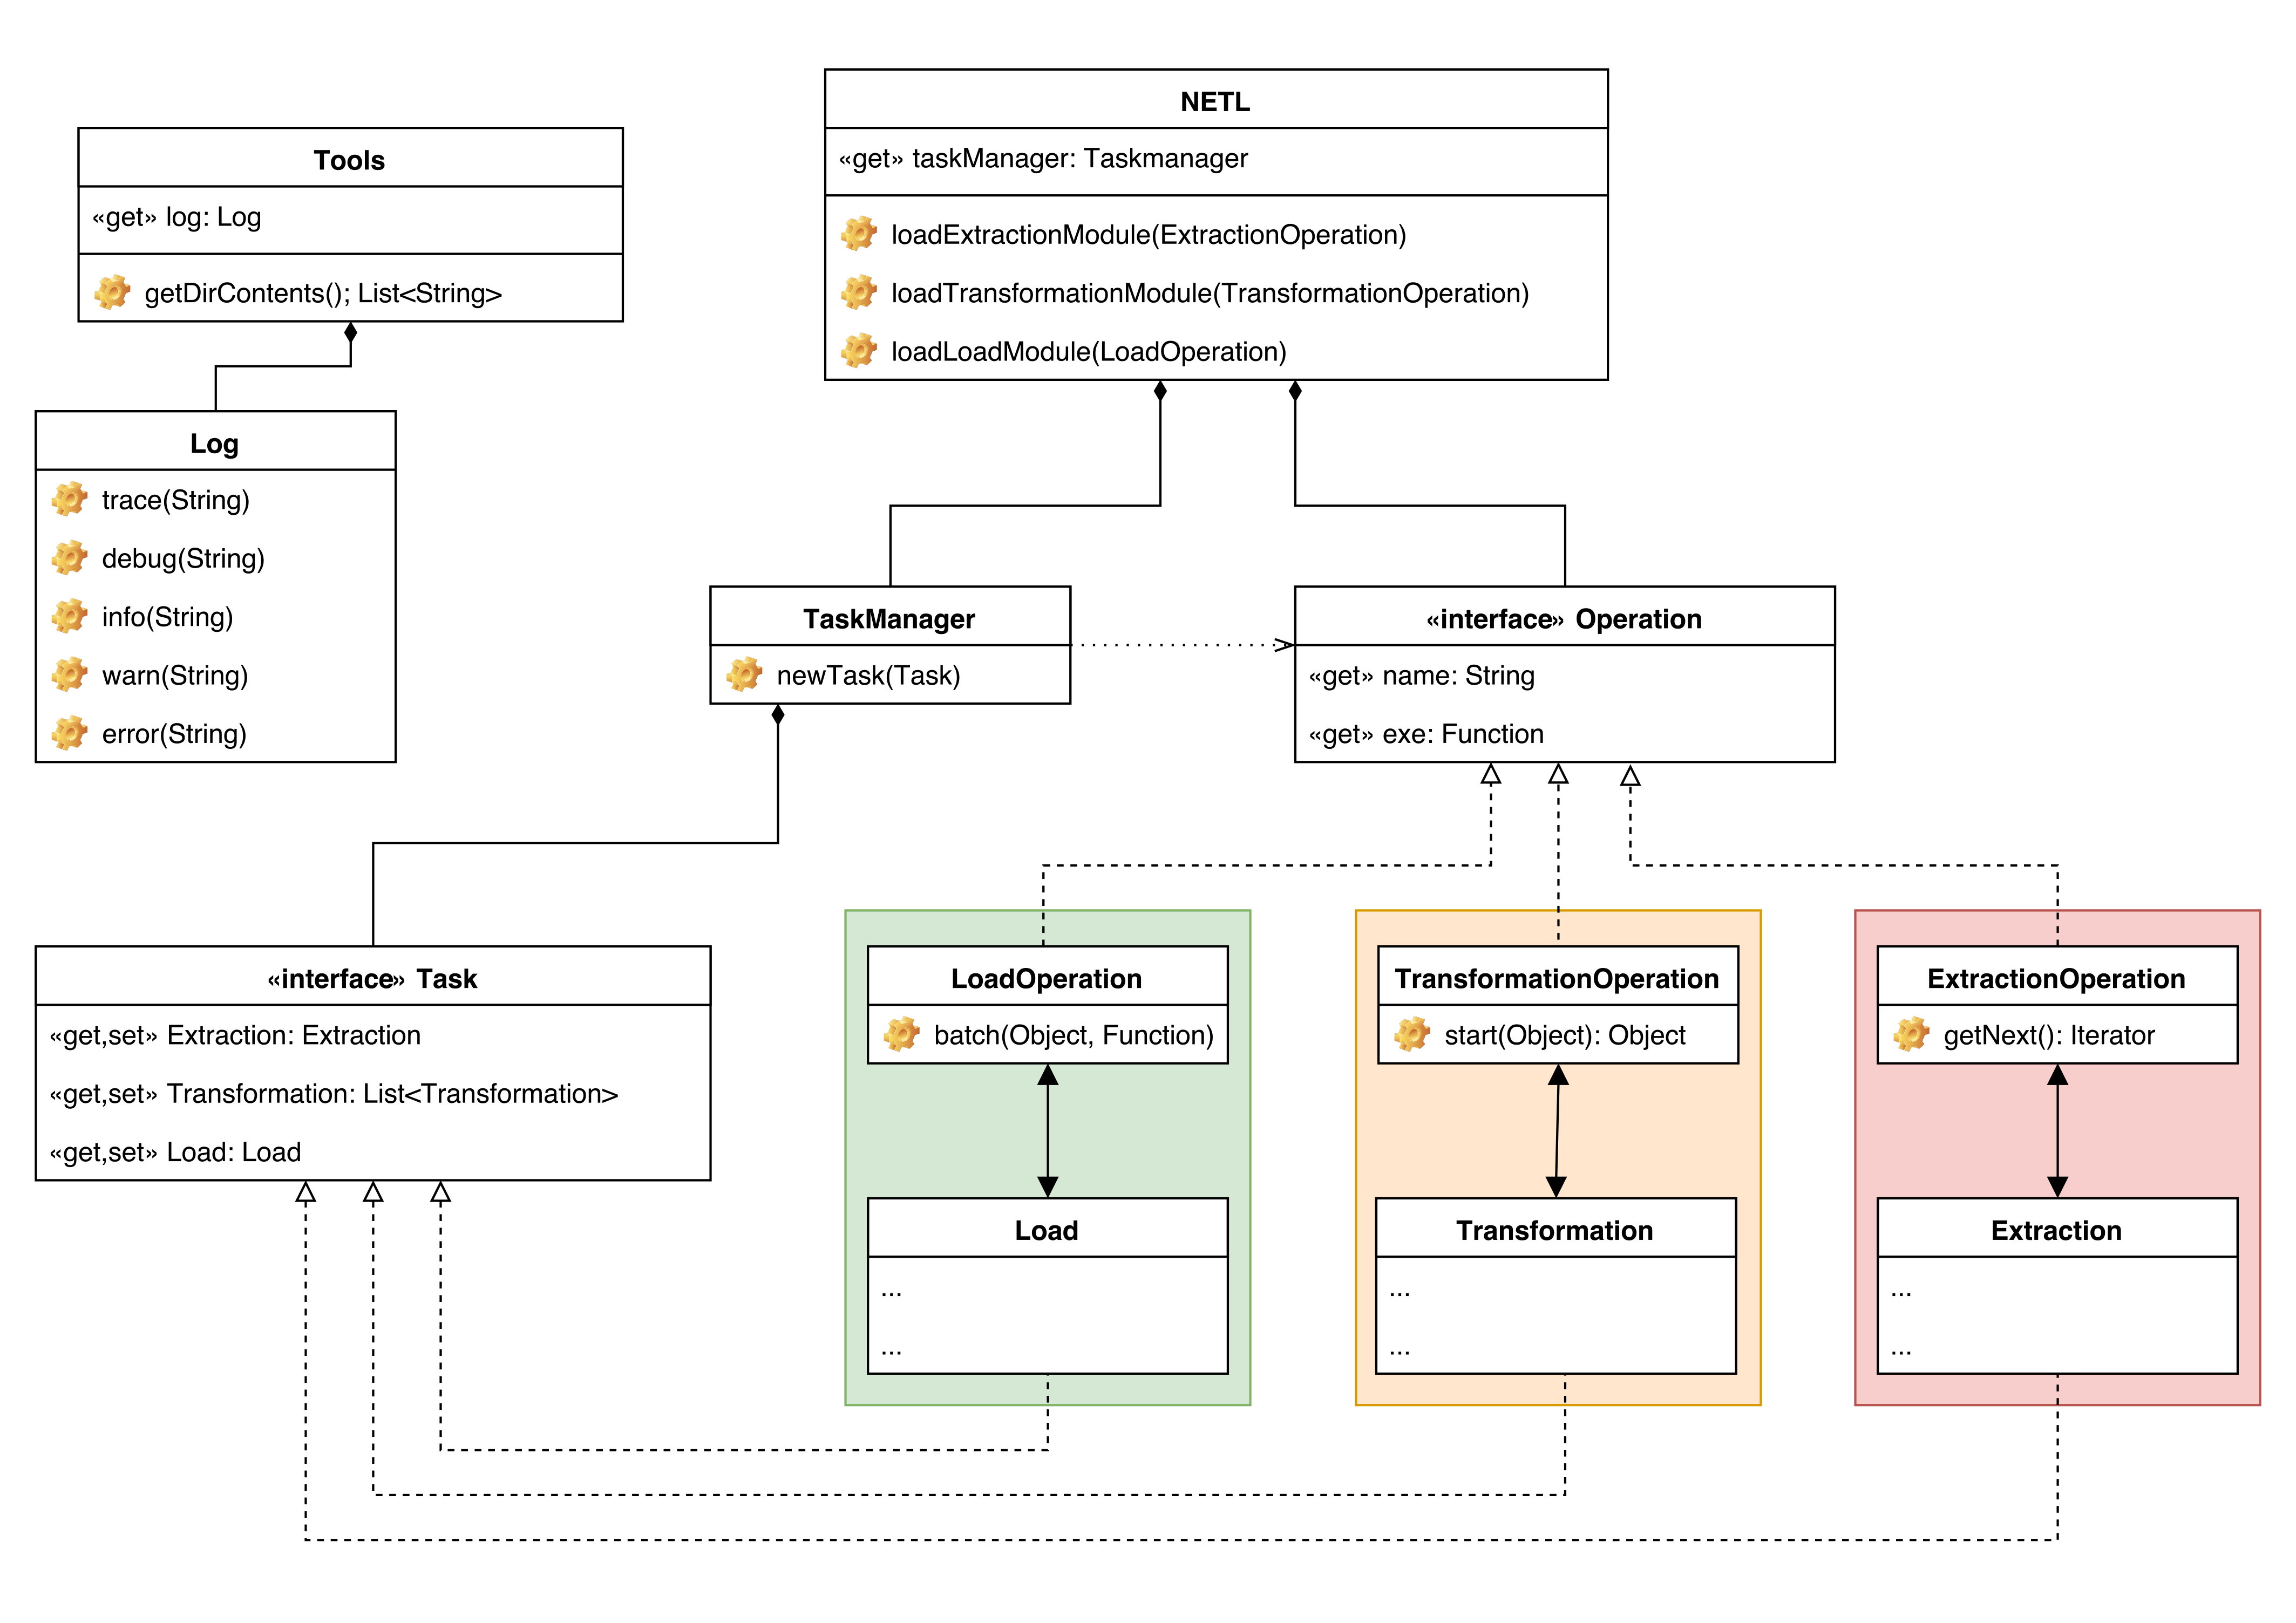
\includegraphics[scale=0.092]{./resources/figures/netlUML.png}
    \end{mdframed}
    \caption[nETL Architecture]{\textbf{Figure \ref{nETL}: nETL Architecture.} \textit{nETL} is an ETL framework designed to host user-created \textit{Modules} to define \textit{extraction}, \textit{transformation} and \textit{loading} processes. \textit{Modules}, shown in the colored boxes, consist of two parts: a configuration object (a JSON object) and a function that adheres to the specified contract. On startup the \textit{nETL} framework loads modules via the operations via a function made available by the main class. The modules are then cached in main memory by the \textit{nETL} process. A user can then interact with the TaskManager class to create a new task via loading a JSON configuration that makes use of a particular \textit{Module}. Tasks consist of an \textit{Extraction module} configuration, several \textit{Transformation module} configurations and a \textit{Load} configuration. Because modules are created and defined by users, as well as the order in which modules are executed, input/output contracts are also defined by the user, and as such \textit{ETL} processes are infinitely configurable.}
    \label{nETL}
\end{figure}

Figure \ref{nETL} shows a potential architecture for a configurable component-based ETL tool, including both the application framework and the E, T, and L operations components. JavaScript is a suitable language to prototype this application for a number of reasons:

\begin{enumerate}
    \item It has a very succinct API making it fast to write code in (i.e. it is a highly abstracted language similarly to Ruby or Python)
    \item But unlike Ruby or Python (and other high level languages), it is opinionated in that it handles IO asynchronously by default
    \item The \textit{JavaScript} implementation of object-orientation is appealing (to some developers at least)
    \item And working and learning \textit{JavaScript} is very much in line with the spirit of CouchDB and the web in general
\end{enumerate}

\subsection{Application Module}
The taskManager object is a simple JavaScript constructor, invoked once on app startup. The resultant object is reference by the main application and made available to the CLI user via closure as is typical when using the JavaScript module patterns. This patterns involves execution of a function and returning references to variables scoped within the function. Since these references remain after function execution the JavaScript garbage collector ignores them. But since they are scoped to the original function call they are private to the referenced return object (JavaScript-eque namespacing). An example of the Application module, instantiation of the taskManager singleton and the \textit{TaskManager} constructor itself is included in the appendix (see \ref{netl-application-module} and \ref{netl-taskmanager-constructor}).

Since IO in JavaScript is asynchronous, batching either needs to be run sequentially (batches are processed one after the other), or by carefully managing asynchronous execution of batches. Batches extracted asynchronously and concurrently would quickly overwhelm the network capabilities of any computer since thousands of network requests would be queued and most would fail. The easier way to handle state in this case (by far!) is serialize processing of batches. As such, nETL is implemented to execute tasks concurrently and asynchronously (not this is not truly parallel execution), and batches of data for a single task serially.

Such an implementation is achieved using JavaScript generators - a means of quickly implementing arbitrary iterators, including iterators over generated iterators \cite{mozillaGenerators} - as a means of serializing iterations over the data source. Once a user directs the application to run a task by the appropriate CLI command with the path to a task configuration specified as an argument, the taskManager object invokes a generator function to return an iterator over the specified data source via the specified \textit{Extraction} operation. This generator function is included in the appendix for reference (See \ref{netl-batch-generator}).

With batch generation serialized, processing each batch via specified E, T and L modules (as per task configuration) is straightforward; first the batch is iterated over, with all transformations applied sequentially to each item. Then the batch is loaded (at once) into the data destination as defined by the task configuration. Because the load operation is allowed to be asynchronous, it is necessary to await the result of the load operation before extracting the next batch. This is done via implementing extraction, transformation, load iteration recursively, with a callback passed to the Load module to re-execute the iterating function on a successful load (the callback is called on resolution of a JavaScript promise in this case). This recursive iterator is included in the appendix (see \ref{netl-recursive-iterator}). All the code snippets included are stripped down and don't include error handling or other code superfluous to the core logic.

\subsection{Extraction, Transformation, Load Modules}
On Module invocation, the contract for E, T, and L operations is that Module execution returns an object with two properties - ``name'': the identifier as used by the application engine to invoke the correct E, T, or L operations during task execution, and the property ``exe'': a pointer to the function that the application engine actually invokes. Closure over the ``exe'' and configuration properties mean that the modules are only evaluated once per task execution (a task may involve calling a transformation function millions of times - once for each item extracted from a CSV), so this is necessarily quite efficient. An example of code defining a module and loading that module into the application is included in the appendix (see \ref{netl-module-loading}).

A list of modules as written for, and used in this project is included in the appendix (see \ref{netl-modules}). Except for the FLATFILE extraction module, they consist of minimal amounts of code with simple logic. The FLATFILE module (see \ref{netl-extract-flatfile} in the appendix) uses a JavaScript generator as a means of serializing CSV line-extraction in regards to the rest of the ETL process. The generator creates an iterator over CSV file content as specified by an open source library available on Github \cite{bower16}.

The most important transformation applied to extracted CSV lines - i.e. the conversion of tabular data into objects uses the TEXT_LINE_TO_OBJ Module (see \ref{netl-trans-text-line-to-obj} in the Appendix). This module makes use of a free CSV parsing library \cite{csvParse} to handle the intricately complex (and necessarily variable) process of properly delimiting CSV content.

Loading data to CouchDB involves a straight forward network request. On the request response a callback as passed to the module is executed to continue the ETL iteration. Due to the cleaner API, Load modules are specifically required to return a promise as part of their contract. The Load Module as used to load data into CouchDB for this project is shown in the appendix (see \ref{netl-load-couchdb}). Network requests make use of the well-known, open-source node.js library ``request'' \cite{request-lib}.
\section{Setup}
Running nETL requires an installation of node.js V8.9.0 +, which should include an installation of npm. After cloning the netl repository from Github to a local drive, dependencies should be restored using the npm CLI tool. Additionally, the directory $C:\log$ needs to be created, and then the nETL app can be started from a terminal. Once the CLI is running, typing anything into the terminal and pressing enter outputs help where further direction can be obtained.

In conjunction with setting up nETL, a CouchDB server needs to be configure. This is easy to do on Windows machines - simply download the executable from apache.org and use the installer. Once installed the server should be run in single node configuration, binded to the 127.0.0.1 address. This allows access to the CouchDB UI via the browser at the address: http://127.0.0.1:5985/\_utils, where first an admin user should be created. Working with databases via the CouchDB interface (called Fauxton) is straightforward.

Database creation involves only the single step of specifying a name and (optionally) security roles. CouchDB database configuration should be specified as part of creation - though this is only available when databases creation is specified via the HTTP interface and not the Fauxton GUI; examples of configurable settings are sharding (q) and replica (n) count, the default of which are configured at the server level. For a single node setup (such as used in this project), q = 8 and n = 1, meaning that a database has 8 shards and only 1 replica of each shard. This is the configuration used in this project; sharding on a single server allows for CouchDB to utilize processes for index calculation. There is not point in storing more than one copy of a single shard on a single server, which is why n = 1 by default for single node CouchDB server.

For CouchDBs operation in cluster mode the default setup is q = 8 and n = 3. For clusters with a large number of nodes it might make sense to increase the value of the q parameter.

\chapter{Analysis}
\section{Overview}
Producing a dataset suitable for analysis involves the workflow specified in \ref{analysis-workflow}. Effectively this is a 3 stage process, where a user configures and runs the \textit{nETL} application to load the data into CouchDB, and then configures a design document with instructions for CouchDB on how to produce an index and emit the contained data in CSV form. Once a CSV of the joined data has been obtained, the final stage of analysis is to load the data into Excel and produce results.

\begin{figure}[ht]
    \centering
    \begin{mdframed}
        \centering
        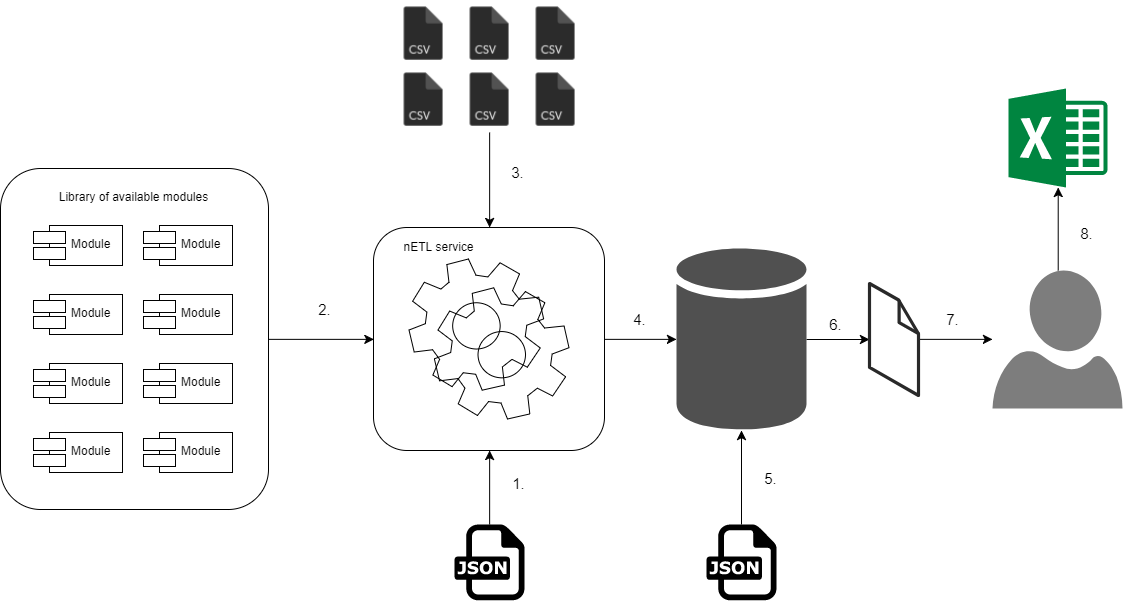
\includegraphics[scale=0.35]{./resources/figures/analysis-workflow.png}
    \end{mdframed}
    \caption[Analysis Workflow]{\textbf{Figure \ref{analysis-workflow}: Workflow to perform an analysis.}1) User creates a configuration file (JSON) that is loaded into the running \textit{\_nETL} service. This configuration includes instructions on which CSVs to load, which modules should be loaded to process the CSVs, and configurations for the modules. 2) Modules are loaded from a library of available modules into the \textit{\_nETL} service. 3) CSVs are loaded into the service, and transformations are applied to the CSV data as specified by the configuration in (1). 4) Data from the CSVs is loaded into CouchDB; this is also achieved via a module specified in (1). 5) A user creates a CouchDB design document, specifying the MapReduce functions, and a List function. 6) The user asks CouchDB to produce the view index as specified by the design document in (5). 7) The user retrieves the data from the view index using the list function specified in (5). 8) The user then loads the resultant CSV into Excel to produce useful metrics.}
    \label{analysis-workflow}
\end{figure}

Analyses are conducted in an iterative fashion; with each iteration an increasing volume of data is handled so as to gain insight into the viability of handling varying amounts of data in CouchDB. Data volume is controlled by the number of courses analyses (more courses taken into account results in higher volumes of data), And the number of entities joined together (grades \& FU data vs grades, FU data, \& Sakai usage). Results are discussed in terms of the insights into business domain (EDM) as well as the effectiveness of the data-mining approach.

\section{Result 1}
This initial analysis is a comparison of student benchmarks (FU data) with CSC1015F course grades.






To maintain the resolution that exists within the Grade data, that is; \textit{results of a particular student in a particular year for a particular course}, joins are performed using a compound key of the tuple [studentID, courseCode, year], i.e. that map functions should emit a key of this tuple.







Configurations used for \textit{nETL} for all the analyses - see \ref{netl-run1-config}). Runtime results of \textit{nETL}, CouchDB indexing times, database/index storage footprints are shown in Table \ref{performance-analysis}.



\section{Join of Grades/Demographics}
Creating datasets comprising grade and FU data involved filtering CSVs and loading that data into CouchDB using \textit{nETL}

For a join on the Grades and Demographics entities, the map function is configured to output key-value pairs of the form: \textless studentID, courseCode, year \textgreater : <9 element list>. A description of the 11-element value list is shown in \ref{grades-join-demographics-output}. Configuration for the \textit{nETL} task is shown in the appendix (see \ref{netl-config-grades-join-demographics}), as is the Map function and list function (see\ref{msc-design-doc}).

The list shown in \ref{grades-join-demographics-output} shows ALL the values output by a map function on the join between all three entities. For the first two runs, event information is NOT emitted.

\begin{figure}[ht]
    \centering
    \begin{minted}{javascript}
 [
    // Grade Entitty output
    "CSC1015F %",

    // Demographic Entity output
    "Gr12 Eng %", 
    "Gr12 Sci %",
    "Gr12 Mth %",
    "Gr12 Mth Lit %",
    "Gr12 Mth Adv %",
    "NBT AL %",
    "NBT QL %",
    "NBT Mth %",

    // Event entity output
    "eventCount S1", // Only included for Run 3/4
    "eventCount S2" // Only included for Run 3/4
 ]    
    \end{minted}
    \caption[2-way-join map output]{\textbf{Figure \ref{grades-join-demographics-output}: Output of map function for grades joined with demographics.} This list, shown as a JavaScript array, is the key to the map function output. In other words, the map function outputs a list of values that correspond to this list. When retrieving the view output, headers can be given back to the columns retrieved using this key. View output can be achieved via a List function (as has been done in this project), or via bespoke JavaScript code.}
    \label{grades-join-demographics-output}
\end{figure}

% Runs
\subsection{CS1015F: Course grades vs Student Benchmarks}


across the FU data and course grades for CSC1015F,


To create the dataset to show correlation between student benchmarking and achieved grades in the CS1015F course for undergraduates, \textit{nETL} was configured to filter Grade data on the field 'Course' to only allow the value 'CS1015F' in addition to the filtering and transforming \textit{nETL} is configured to on all Grade rows as described in the data overview. Additional filtering on the Demographic entity is performed on the StudentID field (anonIdnew) to load demographic data of the students who took the CSC2015F course. This list of students was prepared by Excel filtering, but could just as easily have been performed in CouchDB or any other database if the size of the file did not allow for opening in Excel. Since the view index is small, the list function returns the CSV output instantly. The CSV output size is 67Kb

\subsection{Run 2: Multiple Courses}
With the ease at which the \textit{nETL} software handled loading data in Run 1, and the ease at which CouchDB was able to handle indexing, a second run was created with multiple courses. For this run, 40 courses were selected: ECO1010F, ECO1011S, ACC1006F, STA1000S, ECO2003F, BUS1036F, ECO2004S, CML1001F, MAM1010F, PSY1004F, FTX2024S, ECO2007S, ACC2011S, CSC1015F, PHI2043S, ACC3023S, INF2004F, PSY1005S, STA2020F, CML2010S, CML2001F, SOC1001F, ACC2018S, SOC1005S, BUS2010F, ACC2012W, AXL1100S, ACC3022H, ACC3004H, PHY1012F, MAM1020F, PHI2043F, FTX3045S, ACC3009W, MAM1012S, FTX3044F, MAM1000W, POL1004F, CSC1016S, ACC4000H. These courses were selected simply because they have a high level of student enrollment. \textit{nETL} filtering on the courseCode field was configured to allow all these codes. Filtering on student IDs in the demographic was removed, since over 10 000 student numbers would need to be included a list for such a filter.

Compared to Run1, there is a significant increase in the size footprint of the view index (from \textless 1MB to 143MB) do to the requirement of duplicating demographic output in the map function. Performance of the list function degraded considerably, with streaming of the 2MB CSV taking several minutes. To efficiently retrieve view output of larger indexes would require implementing data retrieval outside of CouchDB. List functions require iterating through every view output individually, whereas working with the view directly would allow for retrieving in batches which is much more efficient. \textit{nETL} could be configured to do this, but hasn't been.

\subsection{Correlation analysis}
The results for \textit{Run 1} and \textit{Run 2} have been summarized in the graphs in Figure \ref{run1-chart1}; several courses were picked at random to show correlation between course grades and student benchmarks. The results show that in general, higher benchmarking scores are indicative of higher course results overall. Some of the benchmarks show stronger correlation to grade results than other, as seen by steeper trendline gradient.

\begin{figure}[H]
    \centering
    \begin{mdframed}
        \centering
        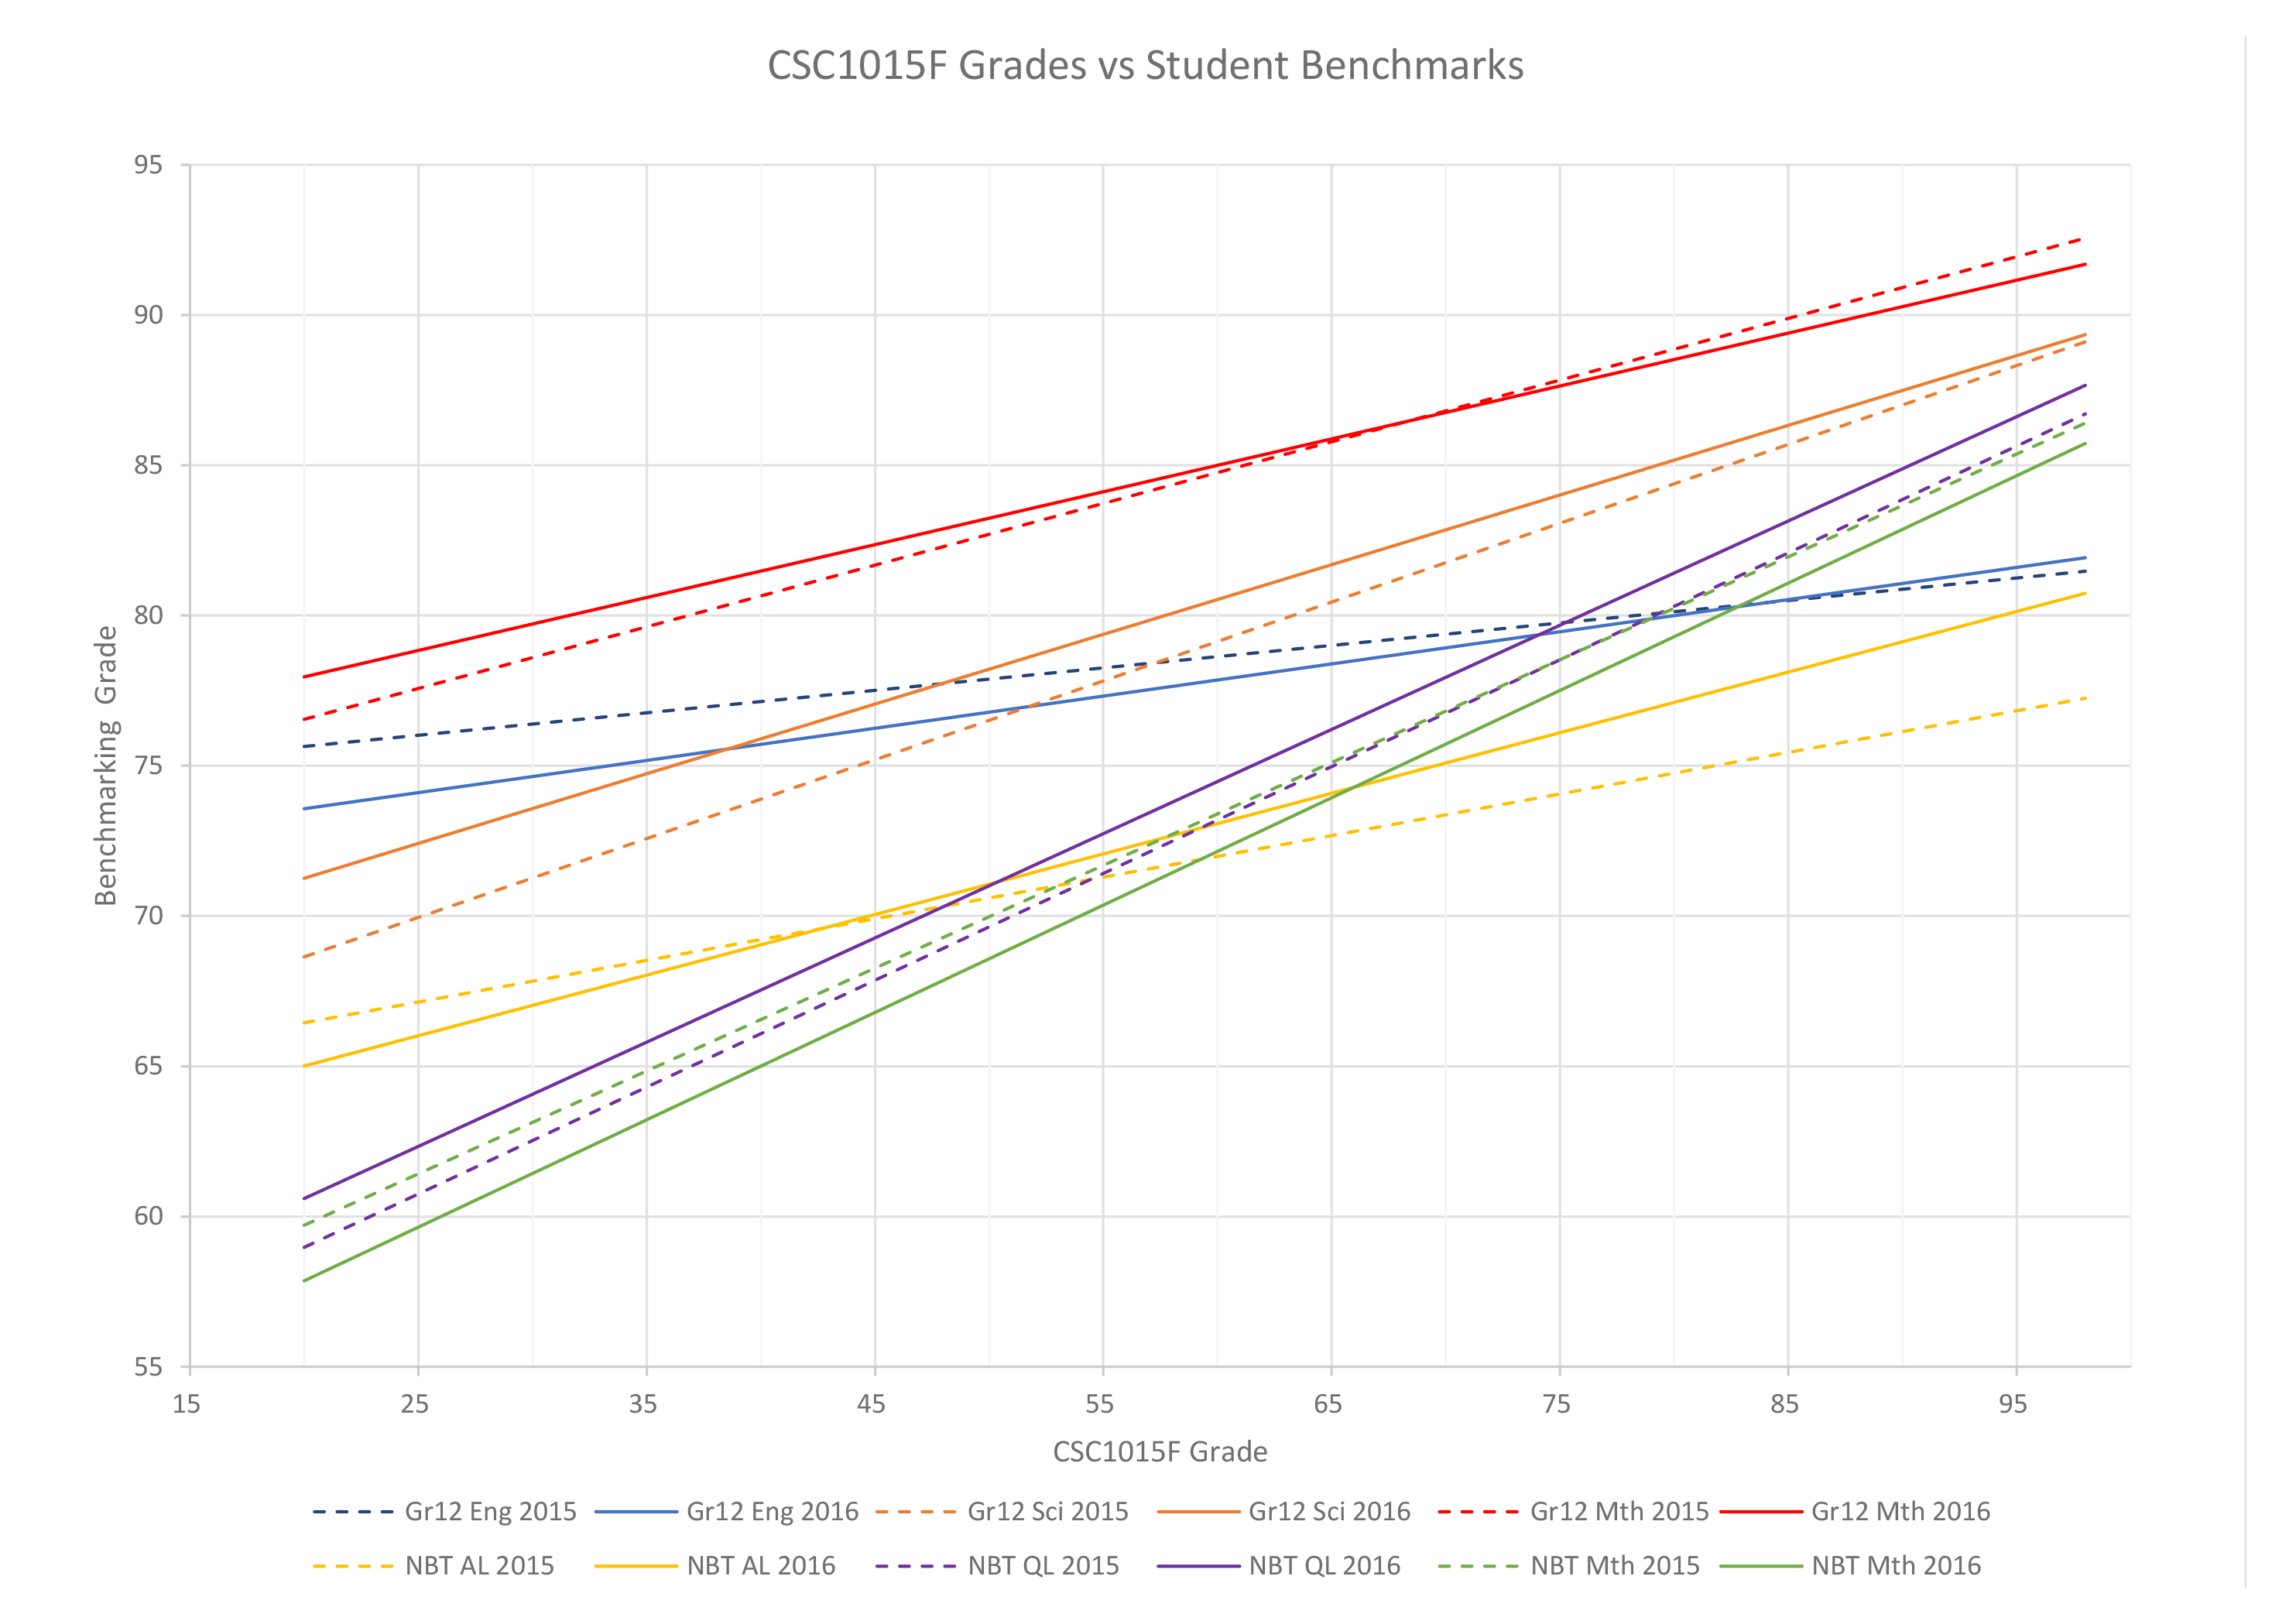
\includegraphics[scale=0.55]{./resources/figures/run1-chart1.png}
    \end{mdframed}
    \caption[CSC1015 grade vs benchmark correlation]{\textbf{Figure \ref{run1-chart1}: Correlation between student benchmarks and CSC1015F results.} This graph shows benchmark scores plotted against the final CSC1015F grade. Datasets focus on a single benchmark, so a trendline shows the correlation between a single benchmark and final grades.}
    \label{run1-chart1}
\end{figure}

\section{join of Grades/Demographics/Events}

% Runs
\subsubsection{Run 3: CS1015F}
Building on the results from \textit{Run 1}, a join on events data was added. To achieve this, n\textit{nETL} was reconfigured to filter grades for only 2016 (since event data is only available for 2016), and an additional \textit{nETL} task was configured to load event data. Filtering on the event data was performed on the (anonymized) uct\_id field to include only events from students who took the CSC1015F course in 2016. This list was derived from the Grade data using Excel.


\subsubsection{Run 4: Multiple Courses}


\subsubsection{Correlation analysis}

\section{2-Way Join}
An initial analysis comparing the correlation between Grade and Benchmark data requires a 2-way join between the Grades and Benchmarks datasets. To achieve this, two nETL tasks were run to extract the CSV data (the ``Grades.CSV'' and ``Benchmarks.CSV'' files) and load rows from these CSV files into CouchDB as documents of type ``grade'' and ``benchmark'' respectively. The JSON configuration file in which both these tasks are defined is included in the appendix at \ref{netl-tasks-1-2-config}. Following loading the data from the CSVs into CouchDB, a Map function is used to produce an index of the CouchDB documents sorted by Student ID, with the guarantee that for every unique student id documents are ordered by type; demographic documents are sorted before Grade documents for for any given student. Knowing the sorted order of documents via the view-index allows for performing the join on data-retrieval. In this retrieval (and joining) is performed via a CouchDB List function (discussed below), with the output in CSV format.

\subsection{nETL Configuration}
The ETL processing of Benchmark data involves an iterative approach of first reading a batch of 10 000 lines from the CSV, performing transformations on each line in the batch, and then loading each batch into CouchDB. On notification that a single batch is loaded successfully into CouchDB, a further 10 000 lines are read from the CSV and processed in the same way. This process continues until the entire CSV has been read and loaded into CouchDB. Batches are loaded into CouchDB via the \textit{\_bulk\_docs}. A list of the progression of transformations applied to each line extracted from each CSV is shown below:

\subsubsection{Task 1 Transformations (Grades)}
\begin{enumerate}
    \item A line is converted into a JavaScript object (which relates directly to the JSON format of CouchDB documents) with the fields:
          \begin{itemize}
              \item DownloadedDate
              \item RegAcadYear
              \item RegTerm
              \item anonIDnew
              \item RegProgram
              \item RegCareer
              \item Degree
              \item DegreeDescr
              \item Subject
              \item Catalog.
              \item Course
              \item CourseSuffix
              \item Session
              \item Percent
              \item Symbol
              \item UnitsTaken
              \item CourseID
              \item CourseDescr
              \item CourseCareer
              \item Faculty
              \item Dept
              \item MaximumCrseUnits
              \item CourseCount
              \item CourseLevel
              \item CESM
              \item Sub-CESM
          \end{itemize}
    \item Lines (now in object form) are filtered on the ``RegCareer'' and ``Course'' fields, where grades achieved for the CSC1015F course taken by students registered as undergrads are considered. Lines that don't meet this attribute are discarded and no further transformations are applied to these line.
    \item An attribute (``type\_'') is then added to each line (that weren't removed in filtering step), and given the value ``grade'' to identify each object as a line of the Grade entity type.
    \item Line attributes are whitelisted. The resultant lines each have the the following attributes:
          \begin{itemize}
              \item type\_
              \item Course
              \item RegAcadYear
              \item anonIDnew
              \item Percent
          \end{itemize}
\end{enumerate}

\subsubsection{Task 2 Transformations (Benchmarks)}
\begin{enumerate}
    \item A line is converted into a JavaScript object with the fields:
          \begin{itemize}
              \item anonIDnew
              \item Career
              \item Citizenship Residency
              \item SA School
              \item Eng Grd12 Fin Rslt
              \item Math Grd12 Fin Rslt
              \item Mth Lit Grd12 Fin Rslt
              \item Adv Mth Grd12 Fin Rslt
              \item Phy Sci Grd12 Fin Rslt
              \item NBT AL Score
              \item NBT QL Score
              \item NBT Math Score
              \item RegAcadYear
          \end{itemize}
    \item Lines are filtered on the ``Career'', ``Citizenship Residency'', and ``anonIDnew'' fields. Only lines for students that attended the CSC1015F course during their undergraduate career and that are either South African citizens or permanent residents are included in the result set. The list of students that attended CSC1015 is derived from the Grade data - this is a manual process since the Grade CSV is small enough that manipulation with Microsoft Excel is possible, and this is only required once (so it's not worth automating).
    \item An attribute (``type\_'') is then added to each remaining line and given the value ``benchmark'' to identify each object as a line of the Benchmark entity type.
    \item Line attributes are whitelisted. The resultant lines each have the the following attributes:
          \begin{itemize}
              \item type\_
              \item anonIDnew
              \item Eng Grd12 Fin Rslt
              \item Math Grd12 Fin Rslt
              \item Mth Lit Grd12 Fin Rslt
              \item Adv Mth Grd12 Fin Rslt
              \item Phy Sci Grd12 Fin Rslt
              \item NBT AL Score
              \item NBT QL Score
              \item NBT Math Score
              \item RegAcadYear
          \end{itemize}
\end{enumerate}

\subsection{MapReduce Functions}
The map function for this analysis is included in the appendix (see \ref{result-1-map}). Each document passed to the map function is treated according to the logic shown in the activity diagram in Figure \ref{result-1-map-fn}. That is, on Map function execution the ``type\_'' attribute is checked. If the document is a line of the Grades entity, then the key [Student ID, year] is emitted along with a single number for the value - the percent achieved for the course. If the document is a line of the Benchmarks entity, then the key [student ID, 0] is emitted along with an ordered list of 8 values corresponding to values for the fields in the Benchmarks.CSV file:

\begin{itemize}
    \item Gr12 English \%
    \item Gr12 science \%
    \item Gr12 Math \%
    \item Gr 12 Math Lit \%
    \item Gr12 Adv Math \%
    \item NBT AL \%
    \item NBT QL \%
    \item NBT Math \%
\end{itemize}

Normalization of the percentage fields (i.e. ``Percent'' for the Grades entity and the test results in the Benchmarks entity) is done via a nested function within the Map function and according to the logic as discussed in that tables previously. No reduce function is used to achieve this 2-way join. This is because, theoretically, a student should only have a single set of Benchmark results and should only achieve a single grade per course per year. As such there is no need to aggregate output from the Map function (which is done via reduction) before performing the document join via the List function.

\begin{figure}[ht]
    \centering
    \begin{mdframed}
        \centering
        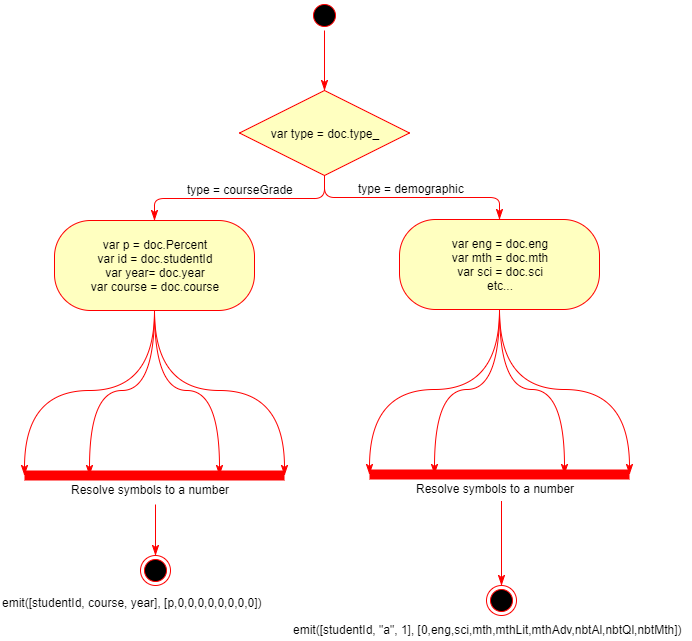
\includegraphics[scale=0.35]{./resources/figures/activity-diagram-1.png}
    \end{mdframed}
    \caption[Result 1 Map function]{\textbf{Figure \ref{result-1-map-fn}: Activity diagram showing logic Map function logic for Results 1 \& 2.} This logic is applied to every document during index calculation (excluding documents with an \_id of ``\_design/*'').}
    \label{result-1-map-fn}
\end{figure}

\subsection{List Function}
TODO

The list function is used to iterate over the results of the MapReduce view, and transform the JSON structure of the view return into a CSV. The list function is included in the appendix (see \ref{result-1-list}). The logic is fairly straight forward; The list function is called via HTTP, specifying the view in the URL, along with the options to group map output by key (at exact level) and to use the reduced result set. The List function first emits a row of headers, as defined in the function itself, and then iterates over the keys in the MapReduce index. For each key, the List function emits a string of comma separated values followed by a newline char according to the RFC 4180 specification. This allows for CSV's to be created and downloaded incrementally allowing for iteration over huge MapReduce indexes.

As mentioned previously List functions are likely to become deprecated in CouchDB. As such it would be better practice to replicate the logic of the List function in a node.js (or alternative) application. If this were to be done, the logic involved in producing a CSV from the MapReduce results would remain the same.
\section{3-Way Join}
Building on the correlation analysis between course grades and benchmarks for CSC1015F, additional information concerning each student's Sakai usage is taken into account. Along with the ``Grades.CSV'' and ``Benchmarks.CSV'' files, a 3rd CSV ``Events.CSV'' is loaded into CouchDB via the nETL application. Since a single student may be associated with many rows in the Event data (sometimes even thousands of rows), a reduce function is used within the MapReduce job to aggregate the Events rows into a single document that is a count of Sakai presence events for first and second semester, with the output of this aggregation (and also the documents for the Grade and Benchmark entities) saved as a view, again, sorted by StudentID. Similarly to the 2-Way analysis of CSC1015F Grade/Benchmarks correlation, a CouchDB List function is used for retrieving data from the view index and performing the 3-way join.

In other words, this analysis addresses the question of whether making more frequent use of the Sakai platform is shown to increase course performance for CSC1015F, as well as looking at the correlation between benchmarking scores and LMS usage. However, the Events cannot be associated with particular courses for the purposes of this study since the Events data FK to course ID, is strictly relevant to the Sakai system only; the grades data has not been exported directly from the Sakai platform and the id that is referenced by Sakai events is not present in the dataset used. As such, this analysis takes into account only ``general usage'' of the Sakai LMS, and not usage of Sakai for these particular courses.

\subsection{nETL Configuration}
nETL Tasks 1 and 2 are the same as run previously for the 2-Way join, except that only course grades from 2016 are used (since the Events exports is only from 2016). The 3-Way join introduces a 3rd task - Task 5 - in which lines from the ``Events.CSV'' file are extracted, transformed and loaded into CouchDB using the nETL application. Tasks 3, 4 \& 5 as JSON configuration files are included in the appendix at \ref{netl-tasks-3-4-5-config}.

Using nETL, Task 5 execution comprises an iterative extraction of 30 000 lines at a time. Each line from each batch undergoes a series of transformations before the entire batch is loaded into CoucDB via the \textit{\_bulk\_docs} endpoint, following which, the iterative extraction continues. A list of the transformations applied to each line extract from the ``Events.CSV'' file by nETL is shown below:

\subsubsection{Task 5 Transformations (Events)}
\begin{enumerate}
  \item A line is converted into a JavaScript object (which relates directly to the JSON format of CouchDB documents) with the fields:
        \begin{itemize}
          \item event\_date
          \item event\_id
          \item uct\_id
          \item site\_key
          \item ref
        \end{itemize}
  \item Lines are filtered on the ``uct\_id'' and ``event\_id'' fields; only events with an event type of ``presence'' (event\_id = 282) for students enrolled in CSC1015F in 2016 are considered.
  \item An attribute (``type\_'') is then added to each line (that weren't removed in filtering step), and given the value ``event'' to identify each object as a line of the Event entity type.
  \item Line attributes are whitelisted. The resultant lines each have the the following attributes:
        \begin{itemize}
          \item type\_
          \item event\_date
          \item event\_id
          \item uct\_id
          \item site\_key
        \end{itemize}
\end{enumerate}

\subsection{MapReduce Functions}
The map function for this analysis is included in the appendix (see \ref{3-way-join-map-function}). Each document passed to the map function is treated according to the logic shown in the activity diagram in Figure \ref{fig-3-way-join-map-function}. Logical handling of the Grade and Benchmark entities is discussed previously.If the document is a line of the Events entity then the date of the event is categorized as either having occurred in semester 1 or semester 2. A key of [Student ID, 0, Year] is emitted along with the value (a 2-index tuple) of [S1, S2]. The S1, and S2 variables are 0 by default, and depending on the date of the presence event, one of these variables is altered to be `1'.

Using the \_sum reduce function, an aggregation is done across all documents with the same key; this means that per a student, an aggregation is performed on a single Grade document, a single Benchmark document, and many Events documents in which the S1 and S2 variables are summed to form the tuple [sum of S1, sum of S2]. Because of the key output of each type of entity, the resulting view-index is ordered by StudentID; for each StudentID documents are ordered by the second index in the key output (course), which means that Benchmarks and Events entities are sorted to be before grades for a student; and sorting via the 3rd index of each key results in benchmark data always being sorted to be before Events documents. As such, during view-index retrieval it can be taken as given that for a single student ID, first documents of type Benchmark will be retrieved, followed by documents of type Event, followed by documents of type Grade.

\subsection{List Function}
The List function is invoked via an HTTP request to the URI: \texttt{https://localhost:5984/msc/\_design/3-way-join/\_list/3-way-join-list/3-way-join-view?reduce=true}. On execution the list function executes the ``provides'' function, in which output type of ``CSV'' (plain text) is specified as as download file. List function logic as shown in Figure \ref{fig-3-way-join-list-function} is executed in the callback passed as a parameter to the ``provides'' function.

On initial invocation and within the body of the callback, the variables `currentStudent', `currentYear', and `currentLine' are set to null. Following this an iteration over the index is initiated within a while loop with the loop invariant the result of a call to the ``getRow'' function. While the loop invariant remains true (i.e. so long as the ``getRow'' function returns a row and not `false', which occurs after the last row has been retrieved from the index), a row - a reduced result - is processed (in the URI the parameter ``reduce'' is set to true, so ONLY reduced output is retrieved from the view). Similarly to List function logic for the 2-way join, after the loop invariant becomes false the last line is still in memory and is sent if necessary.

For every result retrieved from the reduce output , the StudentID of the row being processed is checked and compared to the StudentID of the previous row. If the current StudentID is not the same as the previous StudentID, a line of the CSV is emitted before the row is processed. Then, the type of result being processed is checked (either the document is of type ``benchmark'', ``event'' or ``grade''), and depending on the type different values are stored in a variable called ``currentLine''. For every StudentID, all types of documents are processed in turn (first the benchmark documents, then the event documents, then the grade documents) before being emitted. This allows the join to be performed via sequentially adding to the ``currentLine'' variable for a single student.

As as result of the MapReduce function, for every StudentID, exactly one ``benchmark'' result and one ``event'' document is processed. But a student can have several ``grade'' documents if the course was repeated in subsequent years. To catch this case, when processing documents of type ``grade'' within the switch statement, a further check is done to see if the attribute `year' of the current row has already been processed and is different from a preceding row. If so, the ``currentLine'' is emitted and the fields relating to grade documents are reset, and then repopulated with values from the current row (``currentLine'' itself is not reset). For every Event row processed both the first and second semester event count are exported to the CSV despite that only the first semester events are used, since there is negligible performance cost in terms of processing time or storage space and so there is little incentive to discard good data.

Conceptually, sending ``currentLine'' involves a call to a helper function provided within the execution context of CouchDB List functions - the ``send'' function. This function is wrapped within a subroutine (a function nested within the callback) that first checks that the currentLine variable contains data from the Grades and Benchmarks and Events entity, and then sends a comma-delimited string along a stay-alive network request - this is handled automatically by the HTTP client, which in the case of this project is simply the Google Chrome browser. From a user's perspective, it appears that a file is simply being downloaded; the rate at which the file downloads is equal to the rate at which the loop data is output by the send function. The download completes on completion of the List function.

Code for the loop function is included in the appendix at \ref{3-way-join-list-function}.

\subsection{Output}
A sample of the resultant joined dataset is shown in Figure \ref{fig-3-way-csv-output}
\begin{figure}[H]
    \centering
    \begin{mdframed}[rightline=false,leftline=false]
        \centering
        \begin{BVerbatim}[fontsize=\tiny]

+------+---------+----------+-------+----------+----------+----------+--------------+--------------+--------+--------+---------+------+------+
| Year |   ID    |  Course  | Grade | Gr12 Eng | Gr12 Sci | Gr12 Mth | Gr12 Mth Lit | Gr12 Mth Adv | NBT AL | NBT QL | NBT Mth |  S1  |  S2  |
+------+---------+----------+-------+----------+----------+----------+--------------+--------------+--------+--------+---------+------+------+
| 2016 | 2862568 | CSC1015F |    63 |       80 |        0 |       95 |            0 |            0 |     78 |     79 |      82 |  330 |  138 |
| 2016 | 2864266 | CSC1015F |    64 |       55 |        0 |       74 |            0 |            0 |     59 |     66 |      61 |  557 |  620 |
| 2016 | 2924430 | CSC1015F |    56 |       69 |       94 |       96 |            0 |            0 |     49 |     64 |      77 |  550 |  306 |
| 2016 | 2925212 | CSC1015F |    60 |       76 |        0 |       77 |            0 |            0 |     69 |     84 |      73 |  124 |  155 |
| 2016 | 2928032 | CSC1015F |    30 |       76 |        0 |       73 |            0 |            0 |     85 |     53 |      35 |  307 |  296 |
| 2016 | 2930116 | CSC1015F |    91 |       89 |       91 |       93 |            0 |            0 |     81 |     94 |      94 |  228 |  188 |
| 2016 | 2932174 | CSC1015F |    65 |       79 |        0 |       80 |            0 |            0 |     50 |     64 |      55 |  220 |  225 |
| 2016 | 2932204 | CSC1015F |    30 |       79 |        0 |       84 |            0 |            0 |     66 |     59 |      71 |   78 |    2 |
| 2016 | 2934500 | CSC1015F |    61 |       85 |        0 |       87 |            0 |            0 |     63 |     65 |      78 | 1054 | 1019 |
| 2016 | 2941940 | CSC1015F |    48 |       69 |        0 |       76 |            0 |            0 |     71 |     68 |      69 |  556 |  725 |
| 2016 | 2943800 | CSC1015F |    58 |       67 |        0 |       79 |            0 |            0 |     72 |     65 |      77 |  463 |  531 |
| 2016 | 2944396 | CSC1015F |    61 |       87 |        0 |       82 |            0 |            0 |     69 |     76 |      84 |  935 | 1252 |
| 2016 | 2944854 | CSC1015F |    67 |       82 |        0 |       92 |            0 |            0 |     74 |     83 |      79 |  336 |  264 |
| 2016 | 2946538 | CSC1015F |    48 |       77 |        0 |       74 |            0 |            0 |     77 |     64 |      56 |  533 |  242 |
| 2016 | 2950404 | CSC1015F |    89 |       80 |       75 |       91 |            0 |            0 |     83 |     74 |      85 |  164 |   93 |
| 2016 | 2951308 | CSC1015F |    30 |       80 |        0 |       71 |            0 |            0 |     70 |     62 |      54 |  130 |   50 |
| 2016 | 2951954 | CSC1015F |    42 |        0 |        0 |        0 |            0 |            0 |     78 |     86 |      57 |  309 |   58 |
+------+---------+----------+-------+----------+----------+----------+--------------+--------------+--------+--------+---------+------+------+

        \end{BVerbatim}
    \end{mdframed}
    \caption[Sample of 3-way CSV output]{\textbf{Figure \ref{fig-3-way-csv-output}: Sample of the 3-way join output CSV.} List function output is a CSV download with the schema as represented in this figure. The full CSV has 586 rows (including a header row). Since only a single year of data was analyzed, there are no repeated StudentIDs in the dataset.}
    \label{fig-3-way-csv-output}
\end{figure}


% Figures
\begin{figure}[]
    \centering
    \begin{mdframed}
        \centering
        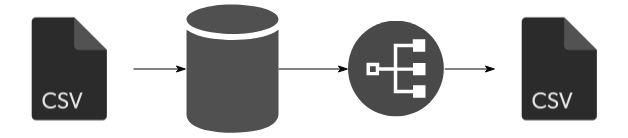
\includegraphics[scale=0.35]{./resources/figures/analysis.png}
    \end{mdframed}
    \caption[Analysis Workflow]{\textbf{Figure \ref{analysis}: Workflow to perform an analysis.} The analysis process represented as a simple pipeline. First nETL extracts data from CSV files and loads that into a CouchDB database via the CouchDB server API. This file consists of a B+tree organized by the \_id field of each document created as a UUID on document write by CouchDB to guarantee uniqueness of every document. From the database file an index is created, also structured as a B+tree but organized by a key as a specified in the Map Function. This allows for sorted output according to a users requirements. A List function is used to retrieve the contents of the view, transform those contents into tabular (CSV) form. The result of calling the List function is a downloaded CSV file. The List function address (API) is of the form \texttt{http(s)://<host>:<port>/<db>/\_design/<doc>/\_list/<fn>/<view>?<params>}}
    \label{analysis}
\end{figure}
\begin{figure}[H]
    \centering
    \begin{mdframed}
        \centering
        \begin{verbatim}
// Map output
[<ID>, ‘0’, 1]: [0, b1, b2, b3, b4, b5, b6, b7, b8, 0, 0]
[<ID>, ‘0’, <Year>]: [0, 0, 0, 0, 0, 0, 0, 0, 0, 1, 0]
[<ID>, ‘0’, <Year>]: [0, 0, 0, 0, 0, 0, 0, 0, 0, 1, 0]
[<ID>, ‘0’, <Year>]: [0, 0, 0, 0, 0, 0, 0, 0, 0, 0, 1]
[<ID>, ‘0’, <Year>]: [0, 0, 0, 0, 0, 0, 0, 0, 0, 0, 1]
[<ID>, ‘0’, <Year>]: [0, 0, 0, 0, 0, 0, 0, 0, 0, 0, 1]
[<ID>, ‘0’, <Year>]: [0, 0, 0, 0, 0, 0, 0, 0, 0, 1, 0]
[<ID>, ‘CSC1015F’, <Year>]: [98, 0, 0, 0, 0, 0, 0, 0, 0, 0, 0]
[<ID>, ‘MAM100F, <Year>]: [94, 0, 0, 0, 0, 0, 0, 0, 0, 0, 0]

// Resulting reduce output
[<ID>, ‘0’, 1]: [0, b1, b2, b3, b4, b5, b6, b7, b8, 0, 0]
[<ID>, ‘0’, <Year>]: [0, 0, 0, 0, 0, 0, 0, 0, 0, 3, 3]
[<ID>, ‘CSC1015F’, <Year>]: [98, 0, 0, 0, 0, 0, 0, 0, 0, 0, 0]
[<ID>, ‘MAM100F, <Year>]: [94, 0, 0, 0, 0, 0, 0, 0, 0, 0, 0]
        \end{verbatim}
    \end{mdframed}
    \caption[Aggregation By Sorted MapReduce output]{\textbf{Figure \ref{mapreduce-key-output}: Aggregating via a combination of MapReduce and relying on sorted B+tree keys.} The Map function should output keys in the form [ID, Course, Year] as shown above for all document processed. However this is not possible for document of type Benchmark (which don't include properties for Course or Year) or documents of type Events (which don't include the property Course). As such, a key of the required format is simply created so as to assure ordering of documents in the resultant B+tree index; in this case documents will all be ordered by Student ID, since all documents contain that property. For Benchmark data, the value `0' is emitted for Course since that value will result in the Benchmark data ordered before documents with a Course property. For the Year field, the value `1' is emitted for Benchmark data since that guarantees ordering of documents by year ahead of any real years. Likewise for documents of type Events, the value `0' is emitted for Course. The resultant B+tree index guarantees that for a particular ID, Benchmark output will occur before Event output which will occur before Grade output.}
    \label{mapreduce-key-output}
\end{figure}
\begin{figure}[ht]
    \centering
    \begin{mdframed}
        \centering
        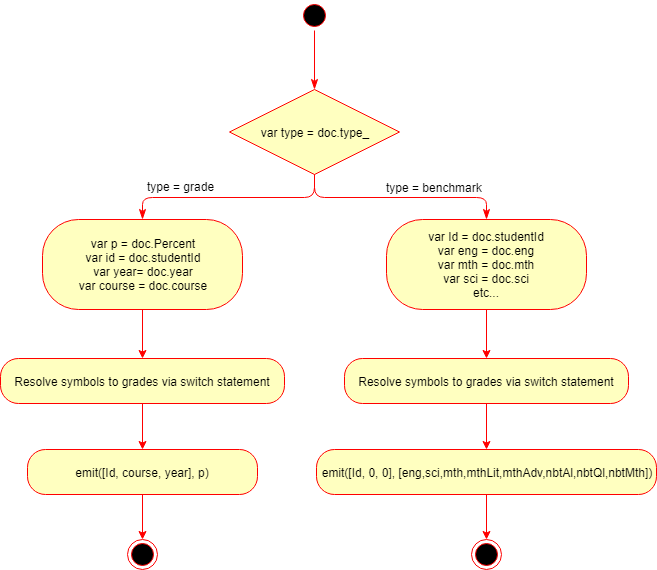
\includegraphics[scale=0.35]{./resources/figures/2-way-join-map.png}
    \end{mdframed}
    \caption[2-Way Join Map Function]{\textbf{Figure \ref{2-way-join-map-fn-diagram}: Map function logic required for the 2-way join.} This logic is applied to every document during index calculation (excluding documents with an \_id of ``\_design/*''). The logic used to normalize grades-as-symbols to percentages is shown in Table \ref{tbl-grades-normalize} for the Grades data, and \ref{tbl-benchmarks-normalize} for the Benchmarks data.}
    \label{2-way-join-map-fn-diagram}
\end{figure}
\begin{figure}[ht]
    \centering
    \begin{mdframed}
        \centering
        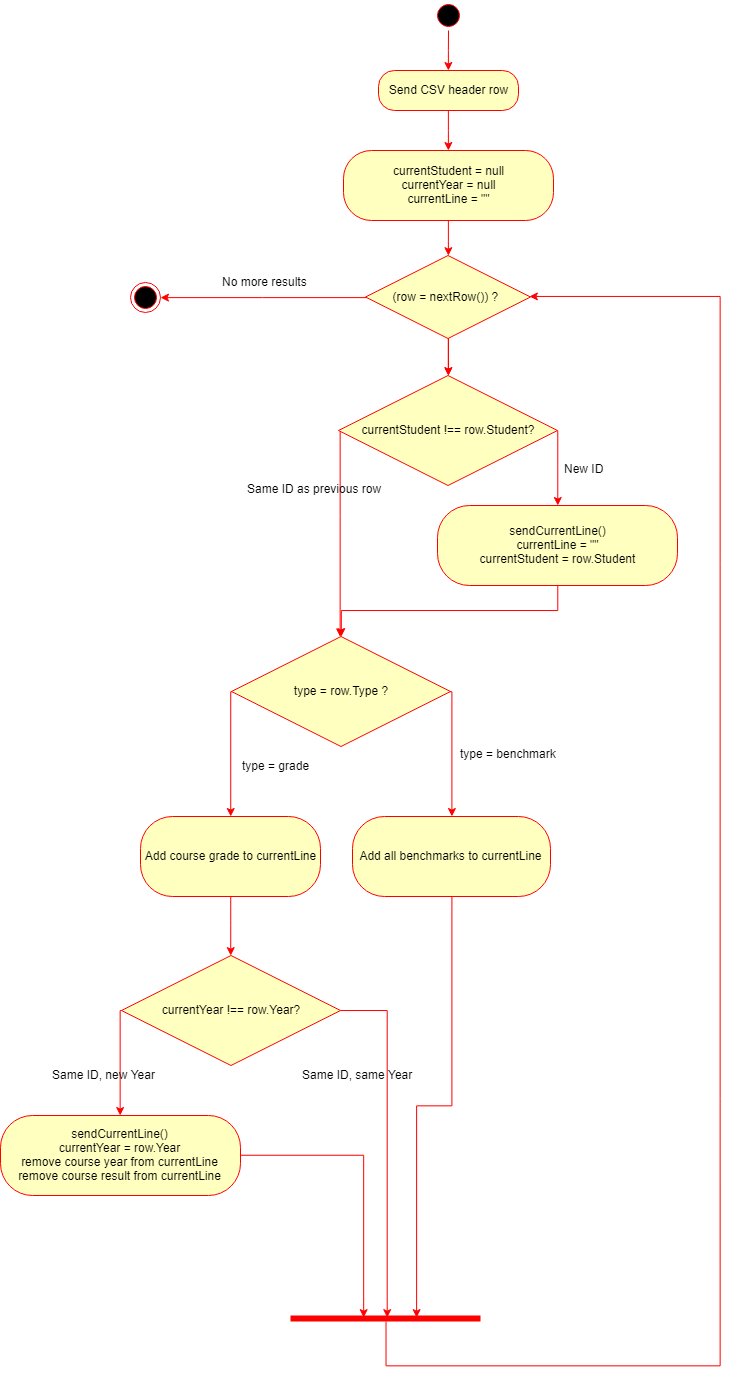
\includegraphics[scale=0.35]{./resources/figures/2-way-join-list.png}
    \end{mdframed}
    \caption[2-Way Join List Function]{\textbf{Figure \ref{fig-2-way-join-list-function}: List function logic required to join the Grades and Benchmarks entities.} Activity diagram of the code executed within the callback passed to the provides function executed by CouchDB during runtime of List function.}
    \label{fig-2-way-join-list-function}
\end{figure}
\begin{figure}[ht]
    \centering
    \begin{mdframed}
        \centering
        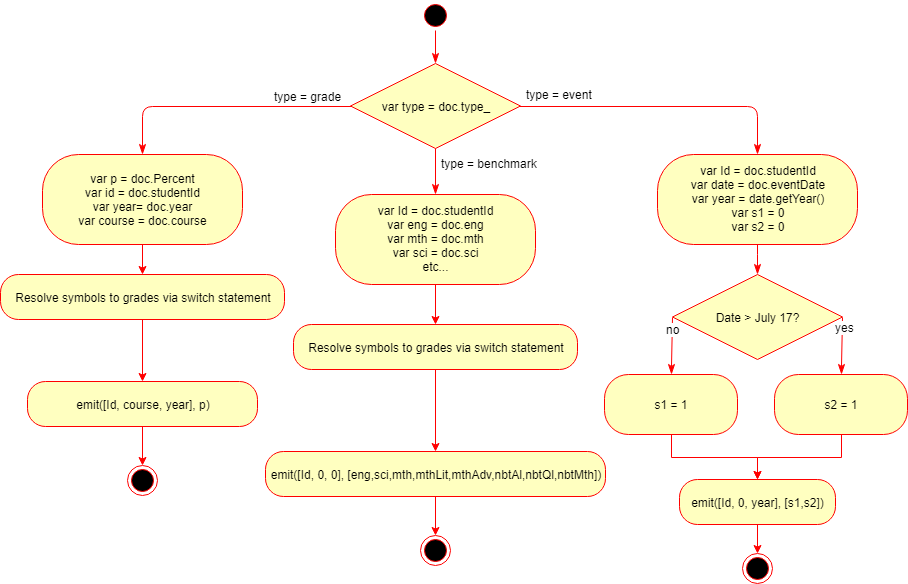
\includegraphics[scale=0.35]{./resources/figures/3-way-join-map.png}
    \end{mdframed}
    \caption[2-Way Join Map Function]{\textbf{Figure \ref{fig-3-way-join-map-function}: Map function logic required for the 2-way join.} This logic is applied to every document during index calculation (excluding documents with an \_id of ``\_design/*''). The logic used to normalize grades-as-symbols to percentages is shown in Table \ref{tbl-grades-normalize} for the Grades data, and \ref{tbl-benchmarks-normalize} for the Benchmarks data.}
    \label{fig-3-way-join-map-function}
\end{figure}
\begin{figure}[H]
    \centering
    \begin{mdframed}
        \centering
        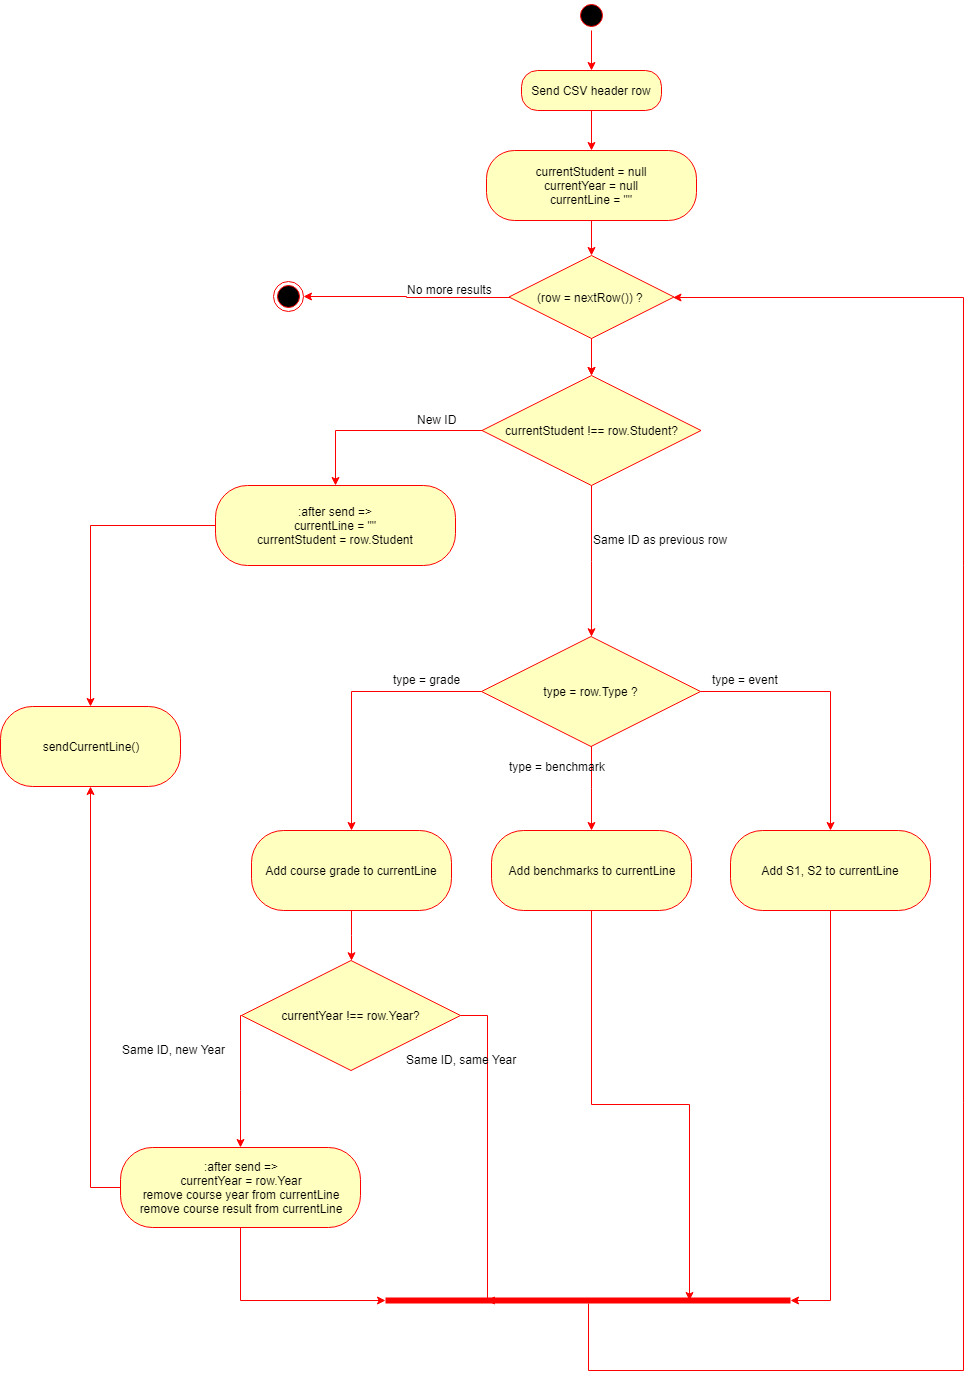
\includegraphics[scale=0.35]{./resources/figures/3-way-join-list.png}
    \end{mdframed}
    \caption[3-Way Join List Function]{\textbf{Figure \ref{fig-3-way-join-list-function}: List function logic required to join the Grades, Benchmarks and Events entities.} Activity diagram of the code executed within the callback passed to the provides function executed by CouchDB during runtime of List function.}
    \label{fig-3-way-join-list-function}
\end{figure}

% Tables
\begin{table}[H]
    \begin{threeparttable}
        \textbf{Table \ref{performance-analysis}}\par\medskip\par\medskip
        \caption[Software performance analysis]{Running time analysis of \textit{nETL} tasks and CouchDB MapReduce indexing}
        \label{performance-analysis}
        \begin{tabularx}{\textwidth}{>{\hsize=1.8\hsize}X>{\hsize=0.8\hsize}Y>{\hsize=0.8\hsize}Y>{\hsize=0.8\hsize}Y>{\hsize=0.8\hsize}Y}
            \toprule
            \mC{c}{}                                               & \mC{c}{2-Way Join} & \mC{c}{3-Way-join}             & \mC{c}{Variance} & \mC{c}{Tests} \\
            \midrule
            Demographic lines extracted                            & -                  & -                              & -                &               \\
            Demographic lines loaded                               & -                  & -                              & -                &               \\
            Demographic task time (sec)\tnote{\textsuperscript{1}} & -                  & -                              & -                &               \\
            \midrule
            Grade lines extracted                                  & -                  & -                              & -                &               \\
            Grade lines loaded                                     & -                  & -                              & -                &               \\
            Grade task time (sec)\tnote{\textsuperscript{1}}       & -                  & -                              & -                &               \\
            \midrule
            Events lines extracted                                 & -                  & 44 420 508                     &                  &               \\
            Events lines loaded                                    & -                  & -                              & -                &               \\
            Events task time (sec)\tnote{\textsuperscript{1}}      & -                  & -                              & -                &               \\
            \midrule
            CouchDB footprint (MB)\tnote{\textsuperscript{2}}      & -                  & -                              & -                &               \\
            View calculation time (sec)\tnote{\textsuperscript{3}} & -                  & -                              & -                &               \\
            View size (MB)                                         & -                  & -                              & -                &               \\
            \midrule
            List function output                                   & -                  & 586\tnote{\textsuperscript{4}} & -                & -             \\
            \bottomrule
        \end{tabularx}
        \scriptsize
        \begin{tablenotes}
            \item[\textsuperscript{1}]Tasks are run asynchronously, so time taken includes processing of other tasks in this run. Task run times are printed out to the log
            \item[\textsuperscript{2}]This is representative of the amount of data processed by \textit{nETL}
            \item[\textsuperscript{3}]CouchDB views are calculated per shard. By default a database contains 8 shards (even in single node mode). The log file shows start and end times of view calculations for each shard, the time is taken as time the first shard starts indexing, to the time the last shard stops indexing
            \item[\textsuperscript{4}]This file comprises a unique list of students, each student associated with the joined output.
        \end{tablenotes}
    \end{threeparttable}
\end{table}
\begin{table}[H]
    \begin{threeparttable}
        \textbf{Table \ref{tbl-grades-normalize}}\par\medskip\par\medskip
        \caption{Grade results need to be treated as numbers for the purpose of this analysis, this table shows all different value types and the appropriate treatment for each. Because of the volume of data, it was not checked how many of these symbols apply to undergraduate students specifically, so these cases were handled generically}
        \label{tbl-grades-normalize}
        \begin{tabularx}{\textwidth}{>{\hsize=0.6\hsize}X>{\hsize=1.3\hsize}X>{\hsize=1.1\hsize}X}
            \toprule
            \mC{c}{Symbol} & \mC{c}{Meaning}          & \mC{c}{Handling Logic}                     \\
            \midrule
            49A            & Absent for supplementary & Grade used                                 \\
            49S            & Supplementary pending    & Grade used                                 \\
            50C            & ?                        & Grade used                                 \\
            78             & Grade                    & Grade used                                 \\
            AB             & Absent (fail)            & N/A                                        \\
            ATT            & ?                        & N/A                                        \\
            DE             & Deferred                 & N/A                                        \\
            DPR            & Duly performed refused   & 30\% Grade used\tnote{\textsuperscript{1}} \\
            F              & Fail                     & 40\% Grade used\tnote{\textsuperscript{2}} \\
            GIP            & Thesis only              & N/A                                        \\
            INC            & Incomplete (fail)        & 30\% Grade used\tnote{\textsuperscript{1}} \\
            LOA            & Leave of absence         & N/A                                        \\
            OS             & Outstanding              & N/A                                        \\
            OSS            & Outstanding              & N/A                                        \\
            PA             & Pass (thesis)            & N/A                                        \\
            SAT            & Thesis only              & N/A                                        \\
            UF             & Unclassified Fail        & 49\% Grade used\tnote{\textsuperscript{3}} \\
            UNS            & Thesis only              & N/A                                        \\
            UP             & Unclassified pass        & 45\% Grade used\tnote{\textsuperscript{4}} \\
            \bottomrule
        \end{tabularx}
        \scriptsize
        \begin{tablenotes}
            \item[\textsuperscript{1}]30\% was applied on the estimate that these students wouldn't necessarily have completed the coursework, and that as such this is a `bad' fail
            \item[\textsuperscript{2}]40\% was applied on the estimate that this symbol would apply to students who participated in the course but still failed
            \item[\textsuperscript{3}]49\% was applied on the estimate that this is a `good' fail, in that the UF classification applies to borderline fails
            \item[\textsuperscript{4}]45\% was applied on the estimate that UP is the 'worst' pass, in that from a strictly grade perspective, these students technically failed
        \end{tablenotes}
    \end{threeparttable}
\end{table}
\begin{table}[h]
    \begin{threeparttable}
        \textbf{Table \ref{tbl-benchmarks-normalize}}\par\medskip\par\medskip
        \caption{Logic for transposing grade symbols to numbers for student benchmark data}
        \label{tbl-benchmarks-normalize}
        \begin{tabularx}{\textwidth}{>{\hsize=0.6\hsize}X>{\hsize=1.3\hsize}X>{\hsize=1.1\hsize}X}
            \toprule
            \mC{c}{Symbol} & \mC{c}{Meaning}             & \mC{c}{Handling Logic}  \\
            \midrule
            A*             & The highest mark achievable & A grade of 90\% is used \\
            A              &                             & A grade of 80\% is used \\
            B              &                             & A grade of 70\% is used \\
            C              &                             & A grade of 60\% is used \\
            D              &                             & A grade of 55\% is used \\
            E              & The lowest pass achievable  & A grade of 50\% is used \\
            \bottomrule
        \end{tabularx}
    \end{threeparttable}
\end{table}

\chapter{Discussion}
todo
\section{CSC1015}
\subsection{Grade / Benchmarks Correlation}
A sample of the CSV file containing the joined Grades and Benchmarks datasets as retrieved from CouchDB is shown in Figure \ref{fig-2-way-csv-output}. Using Microsoft Excel's correlation function, correlation between the Grades and various combinations of the Benchmarks data shows that compared to Gr12 results, the NBT scores correlate significantly better with CSC1015F performance. The highest correlation between benchmarking and CSC1015F course results occurs when the NBT scores are averaged, with either the NBT QL or NBT Mth (or both) scores double weighted; such a correlation is 0.50, which is considered a moderate correlation.

A full list of the correlations tested are shown in Table \ref{tbl-2-way-join-correlation}. Because none of the students have grades for the ``G 12 Mth Lit'' and ``G12 Mth Adv'' columns who attended the CSC1015F course, these benchmarks are not taking into account.
\begin{figure}[H]
    \centering
    \begin{mdframed}[rightline=false,leftline=false]
        \centering
        \begin{BVerbatim}[fontsize=\tiny]

+------+---------+----------+-------+---------+---------+---------+-------------+-------------+-------+-------+--------+
| Year |   ID    |  Course  | Grade | G12 Eng | G12 Sci | G12 Mth | G12 Mth Lit | G12 Mth Adv | NBTAL | NBTQL | NBTMth |
+------+---------+----------+-------+---------+---------+---------+-------------+-------------+-------+-------+--------+
| 2015 | 2749802 | CSC1015F |    71 |      79 |      72 |      85 |           0 |           0 |    86 |    94 |     91 |
| 2015 | 2794606 | CSC1015F |    77 |      75 |      84 |      78 |           0 |           0 |     0 |     0 |      0 |
| 2014 | 2854832 | CSC1015F |    87 |      88 |       0 |      97 |           0 |           0 |    81 |    83 |     82 |
| 2014 | 2860166 | CSC1015F |    37 |       0 |       0 |       0 |           0 |           0 |     0 |     0 |      0 |
| 2016 | 2862568 | CSC1015F |    63 |      80 |       0 |      95 |           0 |           0 |    78 |    79 |     82 |
| 2014 | 2863288 | CSC1015F |    81 |      86 |       0 |      93 |           0 |           0 |    82 |    86 |     90 |
| 2015 | 2863336 | CSC1015F |    66 |      71 |      74 |      75 |           0 |           0 |    76 |    78 |     66 |
| 2015 | 2864266 | CSC1015F |    49 |      55 |       0 |      74 |           0 |           0 |    59 |    66 |     61 |
| 2016 | 2864266 | CSC1015F |    64 |      55 |       0 |      74 |           0 |           0 |    59 |    66 |     61 |
| 2014 | 2880284 | CSC1015F |    64 |      68 |       0 |      93 |           0 |           0 |    65 |    92 |     78 |
| 2014 | 2881364 | CSC1015F |    68 |      87 |       0 |      84 |           0 |           0 |    81 |    86 |     73 |
| 2014 | 2882706 | CSC1015F |    85 |      82 |       0 |      97 |           0 |           0 |    83 |    83 |     92 |
| 2014 | 2890964 | CSC1015F |    80 |      74 |       0 |      88 |           0 |           0 |    78 |    88 |     71 |
| 2014 | 2894402 | CSC1015F |    78 |      70 |       0 |      86 |           0 |           0 |    66 |    71 |     70 |
| 2014 | 2894954 | CSC1015F |    87 |      72 |       0 |      94 |           0 |           0 |    81 |    93 |     88 |
| 2014 | 2895244 | CSC1015F |    64 |      77 |       0 |      85 |           0 |           0 |    72 |    54 |     45 |
| 2015 | 2896964 | CSC1015F |    76 |      77 |       0 |      84 |           0 |           0 |    66 |    82 |     71 |
+------+---------+----------+-------+---------+---------+---------+-------------+-------------+-------+-------+--------+

        \end{BVerbatim}
    \end{mdframed}
    \caption[Sample of 2-way CSV output]{\textbf{Figure \ref{fig-2-way-csv-output}: Sample of the 2-way join output CSV.} List function output is a CSV download with the schema as represented in this figure. The full CSV has 1391 rows; 350 rows for the 2014 year, 457 rows for the 2015 year, 586 rows for the 2016 year. Many student IDs are repeated for different years; this occurs when students retake the course in a subsequent year. In this case, due to the nature of the sorted view index from CouchDB, all a student's course attempts are sequential rows.}
    \label{fig-2-way-csv-output}
\end{figure}

\begin{table}[H]
    \begin{threeparttable}
        \textbf{Table \ref{tbl-2-way-join-correlation}}\par\medskip\par\medskip
        \caption[Grade / Benchmark Correlations]{Assessment of correlation between course grades and student benchmarks over the years 2014/2015/2016. A variety of different combinations of benchmarking data is used in order to assess accuracy of different means of benchmarking students}
        \label{tbl-2-way-join-correlation}
        \begin{tabularx}{\textwidth}{>{\hsize=1.4\hsize}X>{\hsize=0.6\hsize}Y}
            \toprule
            \mC{c}{Benchmark Used}                                      & \mC{c}{Correlation} \\
            \midrule
            Gr12 Eng                                                    & 0.15                \\
            Gr12 Sci                                                    & 0.08                \\
            Gr12 Mth                                                    & 0.25                \\
            NBT AL                                                      & 0.33                \\
            NBT QL                                                      & 0.48                \\
            NBT Mth                                                     & 0.45                \\
            \midrule
            Gr12 Results Avg\tnote{\textsuperscript{1}}                 & 0.17                \\
            With double Mth weighting\tnote{\textsuperscript{2}}        & 0.20                \\
            With double Mth \& Sci weighting\tnote{\textsuperscript{3}} & 0.16                \\
            \midrule
            NBT Results Avg                                             & 0.49                \\
            With double NBT AL                                          & 0.47                \\
            With double NBT QL                                          & 0.50                \\
            With double NBT Mth                                         & 0.50                \\
            With double NBT AL/QL                                       & 0.48                \\
            With double NBT AL/Mth                                      & 0.49                \\
            With double NBT QL/Mth                                      & 0.50                \\
            \midrule
            Avg of NBT \& Gr12                                          & 0.37                \\
            With double Gr 12 Mth weighting                             & 0.37                \\
            With double Gr12 Mth \& Gr12 Sci weighting                  & 0.30                \\
            \bottomrule
        \end{tabularx}
        \scriptsize
        \begin{tablenotes}
            \item[\textsuperscript{1}]This is was the original method used to benchmark incoming students
            \item[\textsuperscript{2}]This method has previously been used to benchmark incoming students
            \item[\textsuperscript{3}]This is the currently used method of benchmarking incoming students
        \end{tablenotes}
    \end{threeparttable}
\end{table}

\chapter{Conclusion}
todo
\section{Future work}
This project's scope is limited to a single approach to document joining, to working with a relatively small amount of data and and working in an environment that CouchDB is not necessarily targeted at. Aside from the fact that more case studies using CouchDB will greatly increase insight into how to use CouchDB more generally, there is scope for further development of the research presented here.

As mentioned previously, CouchDB views are optimized when using built-in reduce functions, with custom reduce functions performing most poorly on Windows machines. As this project was completed on the Windows OS, the analysis on how best to aggregate the different entities (grades, demographics and events) was confined to using just the \textit{\_stats} built in reduce function. The output of this function overlaps output of the other two built-in reduce functions (\textit{\_count}, \textit{\_sum} (and provides additional metrics). Using custom reduce functions would greatly increase the number of possible methods of joining entities since output of map functions would not be constrained to match the contracts of the built-in functions. Such an approach shouldn't be discounted considering that on platforms other than Windows, reduce function calculation (whether custom or built-in) represents a small percentage of computer resources used in view calculations overall (see appendix \ref{slack-1-nov}). And in any case, a system that utilizes CouchDB is likely to be based on a cluster of Linux machines rather than a single Windows machine.

Since, for this project, CouchDB was configured to run on a single Windows machine for this project, it would be worth investigating the benefit that clustering CoucDB across many separate nodes provides. Although the database was sharded (CouchDB is configured to use 8 shards by default) and so processed data in parallel, it is likely that deploying shards to separate servers would greatly increase performance and decrease indexing time. CouchDB disperses documents evenly across shards in a random fashion, suggesting that the workload of indexing the documents would be distributed evenly across all the shards of the database (see \ref{slack-7-nov}). It is likely that the larger benefits would be seen with increasing data sizes since there is first the cost of network interactions to overcome if shards were distributed across separate nodes.

There is also scope to develop a user interface for the \textit{nETL} application and launch a competitor to Microsoft's SSDT that is browser based and JSON-based.
\section*{Acknowledgments}
I would like to give special thanks to my project supervisor Associate Professor Sonia Berman - an extremely patient supervisor who had the foresight to push me (at great effort) in the direction that resulted in a completed MSc. I would also like to thank her for the effort she put in in terms of data acquisition and guiding me in designing the research topic. I would also like to thank Jane Hendry and Stephen Marquard for providing the data exports and scrubbing that such exports required. And lastly I would like to thank the many people who helped me with insights into the thesis topic and the technologies I used. Including: Stephanie Honchell, Patrick DeSomma, Guy Bedford, and many of the CouchDB community who took the time to reply to my messages over Slack.
\newpage

% Bibliogrpahy
\bibliographystyle{plain}
\bibliography{bibliography/msc_citations}

% Appendix
\begin{appendices}
    \chapter{nETL}
    \section{nETL Engine}
\subsection{Sequential Batch Iterator}
\label{netl-batch-generator}
\begin{minted}{javascript}
const extraction;
const batches = (function*() {
    var finished = false;
    while (!finished) {
        let data = [];
        for (let i = 0; i < batchSize; i++) {
            let datum = extraction.getNext();
            if (datum.done) {
                finished = true;
                break
            };
            data.push(datum.value);
        };
        log.info("Task : " + key + " : Batch extracted : Batch size : " + data.length);
        yield data;
    };
})();

// Iteratively generate next batch
batch = batches.next();
\end{minted}

\subsection{TaskManager Constructor}
\label{netl-taskmanager-constructor}
\begin{minted}{javascript}
function TaskManager(e, ts, l) {
    this.tasks = {};
    this.extractions = e;
    this.transformations = ts;
    this.loads = l;
};
TaskManager.prototype.newTask = function(task) { /* ... */ };
\end{minted}

\subsection{Main Application Module}
\label{netl-application-module}
\begin{minted}{javascript}
(function() {
    const _extractions = {};
    const _transformations = {};
    const _loads = {};        
    const _taskManager = new TaskManager(_extractions, _transformations, _loads);
    function _loadExtractionModule(eModule){/* ... */};
    function _loadTransformationModule(tModule){/* ... */};
    function _loadLoadModule(lModule){/* ... */};
    return {
        taskManager: _taskManager,
        loadExtractionModule: _loadExtractionModule,
        loadTransformationModule: _loadTransformationModule,
        loadLoadModule: _loadLoadModule
    };
})();
\end{minted}


\subsection{Recursive ETL Iteration}
\label{netl-recursive-iterator}
\begin{minted}{javascript}
const batches; // Assigned elsewhere
const transformations; // Assigned elsewhere
const load; // Assigned elsewhere
(function doEtlTask(self) {
    var payload = [];

    // Extract next batch
    batch = batches.next();
    if (!batch.done) {
        batch = batch.value;
        self.tasks[key]._itemsExtracted += batch.length;
        batch.forEach(function(item) {

            // Do transformations
            transformations.forEach(function(t) {
                item = t.transform(item);
            });
            if (item && item !== {}) payload.push(item);
        });

        // Load to destination
        load.batch(payload)
            .then(function(msg) {
                doEtlTask(self);
            });
    } else {
        // .. Handle end of task execution
    };
})(this); // Bound to TaskManager instance context
\end{minted}

\section{Extraction, Transformation, Load Modules}
\label{netl-modules}

\subsection{Loading a Module}
\label{netl-module-loading}
\begin{minted}{javascript}
// Load the module into memory
memoryObject[userModule.name] = userModule.exe;
// Invoke the module's closure
var loadedModule = memoryObject[userModule.Name].call(userModule);
// Genrate batch from extraction module
var batch = loadedModule.getNext()
// Do transformations on batch
batch = loadedModule.transform(batch);
// Load transformed batch
load.batch(batch).then(function(msg) {}).catch(function(msg) {});
// An example userModule (an extraction module)
userModule = (function() {
    function exe(configurationObj) {
        function getNext() { /* ... */};
        return {
            getNext: getNext
        };
    };
    return {
        name: "MODULE_NAME",
        exe: exe
    };
})();
\end{minted}


\subsection{FLATFILE}
\label{netl-extract-flatfile}
\begin{minted}{javascript}
'use strict';
const fs = require('fs');
const path = require('path');
/**
 * Configuration exampleL
 * "Extraction": {
 *     "Name": "FLATFILE",
 *     "path": "....csv",
 *     "skipHeaderRows": 1,
 *     "bufferSize": 65536,
 *     "batchSize": 10000,
 *     "startFrom": 0,
 *     "afterTaskRunCBs": []
 * }
 */
function FLATFILE() {
    const options = this;
    const skipItems = options.skipHeaderRows || 0;
    const LF = 10;
    const CR = 13;
    var bufferSize = options.bufferSize || 64 * 1024;
    var position = options.startFrom || 0;
    var lines = _readLines();
    var currentLine = -1;

    // Open the file to be extracted
    var fd;
    var fileStats;
    var filesize;
    var filepath;
    try {
        // Try absolute path
        try {
            filepath = path.normalize(options.path)
            fd = fs.openSync(filepath, 'r');
        } catch (error) {
            // Try relative path
            try {
                filepath = path.normalize(path.join(__dirname, options.path));
                fd = fs.openSync(filepath, 'r');
            } catch (error) {
                throw new Error("File at " + options.path + " cannot be found. Please check your configuration");
            };
        };
        fileStats = fs.fstatSync(fd);
        filesize = fileStats.size;
    } catch (error) {
        throw new Error(error.message);
    };

    /* PRIVATE method */
    function* _readLines() {
        var lineBuffer;
        while (position < filesize) {
            let remaining = filesize - position;
            if (remaining < bufferSize) bufferSize = remaining;
            let chunk = new Buffer(bufferSize);
            let bytesRead = fs.readSync(fd, chunk, 0, bufferSize, position);
            let curpos = 0;
            let startpos = 0;
            let lastbyte = null;
            let curbyte;
            while (curpos < bytesRead) {
                curbyte = chunk[curpos];
                if (curbyte === LF && lastbyte !== CR || curbyte === CR && curpos < bytesRead - 1) {
                    yield _concat(lineBuffer, chunk.slice(startpos, curpos));
                    lineBuffer = undefined;
                    startpos = curpos + 1;
                    if (curbyte === CR && chunk[curpos + 1] === LF) {
                        startpos++;
                        curpos++;
                    };
                } else if (curbyte === CR && curpos >= bytesRead - 1) {
                    lastbyte = curbyte;
                };
                curpos++;
            };
            position += bytesRead;
            if (startpos < bytesRead) {
                lineBuffer = _concat(lineBuffer, chunk.slice(startpos, bytesRead));
            };
        };
        // dump what ever is left in the buffer
        if (Buffer.isBuffer(lineBuffer)) yield lineBuffer;
    };

    /* PRIVATE method */
    function _concat(buffOne, buffTwo) {
        if (!buffOne) return buffTwo;
        if (!buffTwo) return buffOne;

        let newLength = buffOne.length + buffTwo.length;
        return Buffer.concat([buffOne, buffTwo], newLength);
    };

    /* PUBLIC method */
    function getNext() {
        var nextLine = lines.next();
        currentLine++;
        while (currentLine <= skipItems - 1) {
            nextLine = lines.next();
            currentLine++;
        };
        if (!nextLine.done) {
            nextLine.value = nextLine.value.toString();
        };
        return nextLine;
    };

    /* API */
    return {
        getNext: getNext
    };
};
module.exports = {
    name: "FLATFILE",
    exe: FLATFILE
};
\end{minted}

% Loads

\subsection{COUCHDB}
\label{netl-load-couchdb}
\begin{minted}{javascript}
'use strict';
const request = require('request');
/**
 * Configuration example:
 * "Load": {
 *     "Name": "COUCHDB",
 *     "username": "admin",
 *     "password": "password",
 *     "server": "localhost",
 *     "port": 5984,
 *     "ssl": false,
 *     "database": "msc",
 *     "afterTaskRunCBs": []
 * }
 */
function COUCHDB() {
    const options = this;
    const username = options.username || null;
    const password = options.password || null;
    const server = options.server || null;
    const protocol = (options.ssl) ? 'https' : 'http';
    const port = (options.port) ? (typeof options.port === 'number') ? options.port : 80 : 80;
    const db = options.database || null;
    const address = protocol + '://' + username + ':' + password + '@' + server + ':' + port + '/' + db;
    function batch(data) {
        var postData = { docs: data };
        var endpoint = '/_bulk_docs';
        var url = address + endpoint;
        return new Promise(function(fulfill, reject) {
            try {
                request({
                    uri: url,
                    method: 'POST',
                    headers: {
                        'Content-Type': 'application/json'
                    },
                    body: JSON.stringify(postData)
                }, function(err, res, body) {
                    var msg;
                    if (err) {
                        reject(err);
                    } else if (res.statusCode !== 201) {
                        reject(res.statusCode);
                    } else {
                        fulfill(res.statusCode);
                    };
                });
            } catch (e) {
                reject(e);
            };
        });
    };
    return {
        batch: batch
    };
};
module.exports = {
    name: 'COUCHDB',
    exe: COUCHDB
};
\end{minted}

% Transformations

\subsection{TEXT\_LINE\_TO\_OBJ}
\label{netl-trans-text-line-to-obj}
\begin{minted}{javascript}
'use strict';
const Readable = require('stream').Readable;
const csvParser = require('csv-parse/lib/sync');
/**
 * Using RFC 4180 CSV definition
 * Configuration example:
 * {
 *     "Name": "TEXT_LINE_TO_OBJ",
 *     "attributeNames": "<list of CSV headers>",
 *     "delimiter": ",",
 *     "textQualifier": "\"",
 *     "escapeChar": "\\",
 *     "afterTaskRunCBs": []
 * }
 */
function TEXT_LINE_TO_OBJ() {
    const t = this;
    const parseOptions = {
        auto_parse: true,
        auto_parse_date: true,
        columns: null,
        comment: '',
        delimiter: t.delimiter,
        escape: t.escapeChar,
        from: 0,
        to: 1,
        ltrim: true,
        rtrim: true,
        max_limit_on_data_read: 128000,
        quote: t.textQualifier,
        relax: true,
        relax_column_count: false,
        skip_empty_lines: true,
        skip_lines_with_empty_values: true
    };
    const keys = csvParser(t.attributeNames, parseOptions)[0];
    function transform(lines) {
        var retObjs = [];
        lines.forEach(function(line) {
            var values = csvParser(line, parseOptions)[0];
            var obj = Object.create(null);
            keys.forEach(function(el, i, arr) {
                obj[el] = values[i];
            });
            retObjs.push(obj);
        });
        return retObjs;
    };
    return {
        transform: transform
    };
};
module.exports = {
    name: 'TEXT_LINE_TO_OBJ',
    exe: TEXT_LINE_TO_OBJ
};
\end{minted}


\subsection{FILTER}
\label{netl-trans-filter}
\begin{minted}{javascript}
'use strict';
/**
 * Configuration looks like this:
 * filterOn: {"key1"; [<list of allowed values>], "key2": [...], ...}
 * filtering can either be done on objects or arrays since
 * arrays 'keys' are treated as indexes
 *
 * Configuration example:
 * {
 *     "Name": "FILTER",
 *     "filterOn": {
 *         "field1": [<list of allowed values>],
 *         "field2": [<list of allowed values>],
 *         etc...
 *     },
 *     "afterTaskRunCBs": []
 * }
 */
function FILTER() {
    const t = this;
    const filterOn = t.filterOn;
    function transform(batch) {
        const transformedBatch = [];
        batch.forEach(function(datum) {
            var includeThisObj = true;
            Object.keys(filterOn).forEach(function(key) {
                if (filterOn[key].indexOf(datum[key]) < 0) {
                    includeThisObj = false;
                }
            });
            if (includeThisObj) transformedBatch.push(datum);
        });
        return transformedBatch;
    };
    return {
        transform: transform
    };
};
module.exports = {
    name: 'FILTER',
    exe: FILTER
};
\end{minted}

\subsection{WHITELIST}
\label{netl-trans-whitelist}
\begin{minted}{javascript}
/**
 * Configuration example:
 * {
 *     "Name": "WHITELIST",
 *     "allowedAttributes": [
 *         "type_", "RegAcadYear", "anonIDnew", "Course", "Percent"
 *     ],
 *     "afterTaskRunCBs": []
 *     } 
 */
'use strict';
function WHITELIST() {
    const t = this;
    var allowedAttributes = t.allowedAttributes;
    function transform(docs) {
        var retDocs = [];
        docs.forEach(function(doc) {
            var newDoc = {};
            for (var attr in doc) {
                if (!doc.hasOwnProperty(attr)) continue;
                if (allowedAttributes.includes(attr)) newDoc[attr] = doc[attr];
            };
            if (Object.keys(newDoc).length !== 0) retDocs.push(newDoc);
        });
        return retDocs;
    };
    return {
        transform: transform
    };
};
module.exports = {
    name: 'WHITELIST',
    exe: WHITELIST
};
\end{minted}

\subsection{CREATE\_OBJ\_FIELD}
\label{netl-trans-create-obj-field}
\begin{minted}{javascript}
'use strict';
/**
 * Configuration example:
 * {
 *     "Name": "CREATE_OBJ_FIELD",
 *     "newAttributes": [
 *         ["type_", "courseGrade"]
 *     ],
 *     "afterTaskRunCBs": []
 * },
 */
function CREATE_OBJ_FIELD() {
    const t = this;
    function transform(batch) {
        const transformedBatch = JSON.parse(JSON.stringify(batch));
        transformedBatch.forEach(function(datum) {
            if (datum.length == 0) return;
            t.newAttributes.forEach(function(attr) {
                // Throw error if key already exists
                if (datum.hasOwnProperty(attr[0])) {
                    throw new Error("New property not allowed!");
                }
                datum[attr[0]] = attr[1]
            });
        });
        return transformedBatch;
    };
    return {
        transform: transform
    };
};
module.exports = {
    name: 'CREATE_OBJ_FIELD',
    exe: CREATE_OBJ_FIELD
};
\end{minted}
    \section{Configuration files}

\subsection{Result 1}
\label{netl-run1-config}
\begin{minted}{json}
[{
    "ID": "2014/15/16 FU: CSC1015F students",
    "Extraction": {
        "Name": "FLATFILE",
        "path": "C:/MSc/Data/Demographics/FU-CombinedGrades-2016Reg.csv",
        "skipHeaderRows": 1,
        "bufferSize": 65536,
        "batchSize": 10000,
        "startFrom": 0,
        "afterTaskRunCBs": []
    },
    "Transformations": [{
            "Name": "TEXT_LINE_TO_OBJ",
            "attributeNames": "anonIDnew,Career,Citizenship Residency,SA School,Eng Grd12 Fin Rslt,Math Grd12 Fin Rslt,Mth Lit Grd12 Fin Rslt,Adv Mth Grd12 Fin Rslt,Phy Sci Grd12 Fin Rslt,NBT AL Score,NBT QL Score,NBT Math Score,RegAcadYear",
            "delimiter": ",",
            "textQualifier": "\"",
            "escapeChar": "\\",
            "afterTaskRunCBs": []
        },
        {
            "Name": "FILTER",
            "filterOn": {
                "Career": ["UGRD", "First Year", "Second Year", "Third Year"],
                "Citizenship Residency": ["SA Citizen", "Permanent Resident", "C", "P"],
                "anonIDnew": ["list of student IDs for students that took CSC1015F in 2014/15/16"]
            },
            "afterTaskRunCBs": []
        },
        {
            "Name": "CREATE_OBJ_FIELD",
            "newAttributes": [
                ["type_", "demographic"]
            ],
            "afterTaskRunCBs": []
        },
        {
            "Name": "WHITELIST",
            "allowedAttributes": [
                "type_",
                "anonIDnew",
                "Eng Grd12 Fin Rslt",
                "Math Grd12 Fin Rslt",
                "Mth Lit Grd12 Fin Rslt",
                "Adv Mth Grd12 Fin Rslt",
                "Phy Sci Grd12 Fin Rslt",
                "NBT AL Score",
                "NBT QL Score",
                "NBT Math Score",
                "RegAcadYear"
            ],
            "afterTaskRunCBs": []
        }
    ],
    "Load": {
        "Name": "COUCHDB",
        "username": "admin",
        "password": "password",
        "server": "localhost",
        "port": 5984,
        "ssl": false,
        "database": "msc_run1",
        "afterTaskRunCBs": []
    }
}, {
    "ID": "2014/15/16 Grades: CSC1015F students",
    "Extraction": {
        "Name": "FLATFILE",
        "path": "C:/MSc/Data/Grades/CombinedGrades.csv",
        "skipHeaderRows": 1,
        "bufferSize": 65536,
        "batchSize": 10000,
        "startFrom": 0,
        "afterTaskRunCBs": []
    },
    "Transformations": [{
            "Name": "TEXT_LINE_TO_OBJ",
            "attributeNames": "DownloadedDate,RegAcadYear,RegTerm,anonIDnew,RegProgram,RegCareer,Degree,DegreeDescr,Subject,Catalog.,Course,CourseSuffix,Session,Percent,Symbol,UnitsTaken,CourseID,CourseDescr,CourseCareer,Faculty,Dept,MaximumCrseUnits,CourseCount,CourseLevel,CESM,Sub-CESM",
            "delimiter": ",",
            "textQualifier": "\"",
            "escapeChar": "\\",
            "afterTaskRunCBs": []
        },
        {
            "Name": "FILTER",
            "filterOn": {
                "RegCareer": ["UGRD"],
                "Course": ["CSC1015F"]
            },
            "afterTaskRunCBs": []
        },
        {
            "Name": "CREATE_OBJ_FIELD",
            "newAttributes": [
                ["type_", "courseGrade"]
            ],
            "afterTaskRunCBs": []
        },
        {
            "Name": "WHITELIST",
            "allowedAttributes": [
                "type_", "Course", "RegAcadYear", "anonIDnew", "Percent"
            ],
            "afterTaskRunCBs": []
        }
    ],
    "Load": {
        "Name": "COUCHDB",
        "username": "admin",
        "password": "password",
        "server": "localhost",
        "port": 5984,
        "ssl": false,
        "database": "msc_run1",
        "afterTaskRunCBs": []
    }
}]
\end{minted}

\subsection{Result 2}
\label{netl-run2-config}
\begin{minted}{json}
\end{minted}

\subsection{Result 3}
\label{netl-run3-config}
\begin{minted}{json}
\end{minted}

\subsection{Result 4}
\label{netl-run4-config}
\begin{minted}{json}
\end{minted}
    \chapter{CouchDB}
    \section{MapReduce Contract}
\label{couchdb-mapreduce-contracts}
\begin{minted}{text}
/**
 * Map function
 * @param  {Object} doc Each document in the database is passed in turn to the function
 * @return {null} Nothing is returned - key:value pairs are emitted (multiple pairs can be emitted per document)
 */
function(doc) {
    emit(someKey, someValue);
};

/**
 * Reduce function (javascript implementation of the _sum function shown)
 * @param  {Object[]} [keys] A list of [key, docId] pairs - key as from the map function, and key from the original doc
 * @param  {Object[]} values Output from the map function, or from the reduce function
 * @param  {Boolean} [rereduce] Indicates whether values are output from the map (rereduce = false) or reduce (rereduce = true) function
 * @return {[type]}
 */
function(keys, values, rereduce) {
    if (rereduce) {
        return values.reduce(function(a,b) {
            return a + b;
        }, 0);
    } else {
        return values.length;
    };
};
\end{minted}

\section{Sample Design Document}
\label{couchdb-design-doc-sample}
\begin{minted}{json}
{
    "_id": "_design/sample",
    "_rev": "xxxxx",
    "language": "javascript",
    "views": {
        "view1": {
            "map": "function(doc) { ... }",
            "reduce": "function(keys, values, rereduce) { ... }"
        },
        "view2": {
            "map": "function(doc) { ... }",
            "reduce": "_stats"            
        }
    },
    "shows": {
        "show1": "function(doc, req) { ... }",
        "show2": "function(doc, req) { ... }"
    },
    "lists": {
        "listFunc1": "function(head, req) { ... };",
        "listFunc2": "function(head, req) { ... };"
    },
    "updates": {
        "update1": "function(doc, req) { ... }",
        "update2": "function(doc, req) { ... }"
    },
    "filters": {
        "filter1": "function(doc, req) { ... }",
        "filter2": "function(doc, req) { ... }"
    },
    "validate_doc_update": "function(newDoc, oldDoc, userCtx, secObj) { ... }"
}
\end{minted}

\section{Design Document Functions}
\subsection{2-Way Join}
\subsubsection{Map Function}
\label{2-way-join-map-function}
\begin{minted}{text}
function(doc) {
    /* Compound key */
    var id;
    var course;
    var year;

    /* Decision tree */
    var type = doc.type_;
    switch (type) {
        case 'grade':

            /* Key */
            id = doc.anonIDnew;
            course = doc.Course;
            year = doc.RegAcadYear;

            /* Value */
            var percent = doc.Percent || '';

            /* Normalize the percent field to a number */
            if (typeof percent !== 'number') {
                if (typeof percent !== 'string') return;
                var percentCleaned = percent.toUpperCase().trim();

                /* Return if percent is a disallowed symbol */
                if ([
                        'ATT',
                        'DE',
                        'GIP',
                        'LOA',
                        'OS',
                        'OSS',
                        'PA',
                        'SAT',
                        'UNS',
                        'AB',
                        ''
                    ].indexOf(percentCleaned) >= 0) return;

                /* Get the percentage */
                switch (percentCleaned) {
                    case 'F':
                        percent = 40;
                        break;
                    case 'DPR':
                        percent = 30;
                        break;
                    case 'INC':
                        percent = 30;
                        break;
                    case 'UF':
                        percent = 49;
                        break;
                    case 'UP':
                        percent = 45;
                        break;
                    default:
                        /* Convert percent to number */
                        percent = parseFloat(percent.substring(0, percent.length - 1));
                        if (isNaN(percent)) return;
                        break;
                };
            };

            /* Output */
            emit([id, course, year], percent);
            break;

        case 'benchmark':

            /* Key */
            id = doc.anonIDnew;
            course = 0;
            year = 0;

            /* Value (each index corresponds to a benchmark) */
            var benchmarks = [0, 0, 0, 0, 0, 0, 0, 0];

            /* Normalize symbols to numbers */
            var fuDictionary = {
                "A*": 90,
                "A": 80,
                "B": 70,
                "C": 60,
                "D": 55,
                "E": 50
            };

            function getDemographicGrade(gr) {
                var g = parseInt(gr);
                var retG;
                if (isNaN(g)) { // True for sumbols
                    if (typeof gr !== 'string') return 0;
                    retG = fuDictionary[gr.toUpperCase().trim()] || 0;
                } else {
                    retG = g;
                };
                return retG;
            };

            // Gr12 Eng
            var gEng12 = getDemographicGrade(doc["Eng Grd12 Fin Rslt"] || "");
            benchmarks[0] = gEng12;

            // Gr12 Sci
            var gSci12 = getDemographicGrade(doc["Phy Sci Grd12 Fin Rslt"] || "");
            benchmarks[1] = gSci12;

            // Gr12 Mth
            var gMth12 = getDemographicGrade(doc["Math Grd12 Fin Rslt"] || "");
            benchmarks[2] = gMth12;

            // Gr12 Mth Lit
            var gMthLit12 = getDemographicGrade(doc["Mth Lit Grd12 Fin Rslt"] || "");
            benchmarks[3] = gMthLit12;

            // Gr12 Mth Adv
            var gMthAdv12 = getDemographicGrade(doc["Adv Mth Grd12 Fin Rslt"] || "");
            benchmarks[4] = gMthAdv12;

            // NBT AL
            var gNbtAl = getDemographicGrade(doc["NBT AL Score"] || "");
            benchmarks[5] = gNbtAl;

            // NBT QL
            var gNbtQl = getDemographicGrade(doc["NBT QL Score"] || "");
            benchmarks[6] = gNbtQl;

            // NBT Mth
            var gNbtMth = getDemographicGrade(doc["NBT Math Score"] || "");
            benchmarks[7] = gNbtMth;

            /* Output */
            emit([id, course, year], benchmarks);
            break;

        default:
            break;
    };
};
\end{minted}

\subsubsection{List Function}
\label{2-way-join-list-function}
\begin{minted}{text}
function(head, req) {
    provides('csv', function() {
        /* Send the headers */
        var headers = "Year,StudentAnonID,Course,Course %,Gr12 Eng %,Gr12 Sci %,Gr12 Mth %,Gr12 Mth Lit %,Gr12 Mth Adv %,NBT AL %,NBT QL %,NBT Mth %";
        send(headers);

        /* Helper function; send current year */
        function sendLine(obj) {
            if (obj.benchmark && obj.grade) {
                var line =
                    "\n" + obj.year +
                    "," + obj.id +
                    "," + obj.course +
                    "," + obj["Course %"] +
                    "," + obj["Gr12 Eng %"] +
                    "," + obj["Gr12 Sci %"] +
                    "," + obj["Gr12 Mth %"] +
                    "," + obj["Gr12 Mth Lit %"] +
                    "," + obj["Gr12 Mth Lit %"] +
                    "," + obj["NBT AL %"] +
                    "," + obj["NBT QL %"] +
                    "," + obj["NBT Mth %"];
                send(line);
            };
        };

        /* Current function scope variables */
        var currentStudent = null;
        var currentYear = null;
        var currentLine = {};
        var key;
        var id;
        var course;
        var year;
        var value;

        /* Iterate through view results */
        while (row = getRow()) {

            /* Key */
            key = row.key;
            id = key[0];
            course = key[1];
            year = key[2];

            /* Value */
            value = row.value;

            /* Send previous line if it's a new student and then reset id */
            if (currentStudent !== id) {
                sendLine(currentLine);
                currentLine = {};
                currentStudent = id;
            };

            /* Append to/adjust current line */
            var type = (course === 0 && year === 0) ? 'benchmark' : 'grade';
            switch (type) {
                case 'benchmark':
                    currentLine.benchmark = true;
                    currentLine.id = id;
                    currentLine["Gr12 Eng %"] = value[0];
                    currentLine["Gr12 Sci %"] = value[1];
                    currentLine["Gr12 Mth %"] = value[2];
                    currentLine["Gr12 Mth Lit %"] = value[3];
                    currentLine["Gr12 Mth Adv %"] = value[4];
                    currentLine["NBT AL %"] = value[5];
                    currentLine["NBT QL %"] = value[6];
                    currentLine["NBT Mth %"] = value[7];
                    break;

                case 'grade':

                    /* Send previous line if it's a new year */
                    if (currentYear !== year) {
                        sendLine(currentLine);
                        currentYear = year;
                    };

                    currentLine.grade = true;
                    currentLine.id = id; // In case no demographic doc exists
                    currentLine.year = year;
                    currentLine.course = course;
                    currentLine["Course %"] = value[0];
                    break;

                default:
                    send({ error: "Document type unexpected" });
                    break;
            };
        };
    });
};
\end{minted}

\subsection{3-Way Join}
\subsubsection{Map Function}
\label{3-way-join-map-function}
\begin{minted}{text}
function(doc) {
    /* Compound key */
    var id;
    var course;
    var year;

    /* Decision tree */
    var type = doc.type_;
    switch (type) {
        case 'grade':
            /* Key */
            id = doc.anonIDnew;
            course = doc.Course;
            year = doc.RegAcadYear;

            /* Value */
            var percent = doc.Percent || '';

            /* Normalize the percent field to a number */
            if (typeof percent !== 'number') {
                if (typeof percent !== 'string') return;
                var percentCleaned = percent.toUpperCase().trim();

                /* Return if percent is a disallowed symbol */
                if ([
                        'ATT',
                        'DE',
                        'GIP',
                        'LOA',
                        'OS',
                        'OSS',
                        'PA',
                        'SAT',
                        'UNS',
                        'AB',
                        ''
                    ].indexOf(percentCleaned) >= 0) return;

                /* Get the percentage */
                switch (percentCleaned) {
                    case 'F':
                        percent = 40;
                        break;
                    case 'DPR':
                        percent = 30;
                        break;
                    case 'INC':
                        percent = 30;
                        break;
                    case 'UF':
                        percent = 49;
                        break;
                    case 'UP':
                        percent = 45;
                        break;
                    default:
                        /* Convert percent to number */
                        percent = parseFloat(percent.substring(0, percent.length - 1));
                        if (isNaN(percent)) return;
                        break;
                };
            };

            /* Output */
            emit([id, course, year], percent);
            break;

        case 'benchmark':
            /* Key */
            id = doc.anonIDnew;
            course = 0;
            year = 0;

            /* Value (each index corresponds to a benchmark) */
            var benchmarks = [0, 0, 0, 0, 0, 0, 0, 0];

            /* Normalize symbols to numbers */
            var fuDictionary = {
                "A*": 90,
                "A": 80,
                "B": 70,
                "C": 60,
                "D": 55,
                "E": 50
            };

            function getDemographicGrade(gr) {
                var g = parseInt(gr);
                var retG;
                if (isNaN(g)) { // True for sumbols
                    if (typeof gr !== 'string') return 0;
                    retG = fuDictionary[gr.toUpperCase().trim()] || 0;
                } else {
                    retG = g;
                };
                return retG;
            };

            // Gr12 Eng
            var gEng12 = getDemographicGrade(doc["Eng Grd12 Fin Rslt"] || "");
            benchmarks[0] = gEng12;

            // Gr12 Sci
            var gSci12 = getDemographicGrade(doc["Phy Sci Grd12 Fin Rslt"] || "");
            benchmarks[1] = gSci12;

            // Gr12 Mth
            var gMth12 = getDemographicGrade(doc["Math Grd12 Fin Rslt"] || "");
            benchmarks[2] = gMth12;

            // Gr12 Mth Lit
            var gMthLit12 = getDemographicGrade(doc["Mth Lit Grd12 Fin Rslt"] || "");
            benchmarks[3] = gMthLit12;

            // Gr12 Mth Adv
            var gMthAdv12 = getDemographicGrade(doc["Adv Mth Grd12 Fin Rslt"] || "");
            benchmarks[4] = gMthAdv12;

            // NBT AL
            var gNbtAl = getDemographicGrade(doc["NBT AL Score"] || "");
            benchmarks[5] = gNbtAl;

            // NBT QL
            var gNbtQl = getDemographicGrade(doc["NBT QL Score"] || "");
            benchmarks[6] = gNbtQl;

            // NBT Mth
            var gNbtMth = getDemographicGrade(doc["NBT Math Score"] || "");
            benchmarks[7] = gNbtMth;

            /* Output */
            emit([id, course, year], benchmarks);
            break;

        case 'event':
            var date = new Date(doc.event_date);
            var epoch = date.getTime();

            /* Key */
            id = doc.uct_id;
            course = 0;
            year = date.getFullYear();

            /* Value */
            var event = [0, 0];

            /* Midpoint =  Sunday, July 17, 2016 10:00:00 PM */
            var midDate = 1468792800000
            var semester = (epoch - midDate >= 0) ? 2 : 1;
            if (semester === 1) {
                event[0] = 1;
            } else {
                event[1] = 1;
            };

            /* Output */
            emit([id, course, year], event);
            break;

        default:
            break;
    };
};
\end{minted}

\subsubsection{List Function}
\label{3-way-join-list-function}
\begin{minted}{text}
function(head, req) {
    provides('csv', function() {
        /* Send the headers */
        var headers = "Year,StudentAnonID,Course,Course %,Gr12 Eng %,Gr12 Sci %,Gr12 Mth %,Gr12 Mth Lit %,Gr12 Mth Adv %,NBT AL %,NBT QL %,NBT Mth %,S1 Events, S2 Events";
        send(headers);

        /* Helper function; send current year */
        function sendLine(obj) {
            if (obj.benchmark && obj.grade) {
                var line =
                    "\n" + obj.year +
                    "," + obj.id +
                    "," + obj.course +
                    "," + obj["Course %"] +
                    "," + obj["Gr12 Eng %"] +
                    "," + obj["Gr12 Sci %"] +
                    "," + obj["Gr12 Mth %"] +
                    "," + obj["Gr12 Mth Lit %"] +
                    "," + obj["Gr12 Mth Lit %"] +
                    "," + obj["NBT AL %"] +
                    "," + obj["NBT QL %"] +
                    "," + obj["NBT Mth %"] +
                    "," + obj.S1 +
                    "," + obj.S2;
                send(line);
            };
        };

        /* Current function scope variables */
        var currentStudent = null;
        var currentYear = null;
        var currentLine = {};
        var key;
        var id;
        var course;
        var year;
        var value;

        /* Iterate through view results */
        while (row = getRow()) {

            /* Key */
            key = row.key;
            id = key[0];
            course = key[1];
            year = key[2];

            /* Value */
            value = row.value;

            /* Send previous line if it's a new student and then reset id */
            if (currentStudent !== id) {
                sendLine(currentLine);
                currentLine = {};
                currentStudent = id;
            };

            /* Append to/adjust current line */
            var type = (course === 0 && year === 0) ?
                'benchmark' : ((course === 0) ?
                    'event' : 'grade');

            switch (type) {
                case 'benchmark':
                    currentLine.benchmark = true;
                    currentLine.id = id;
                    currentLine["Gr12 Eng %"] = value[0];
                    currentLine["Gr12 Sci %"] = value[1];
                    currentLine["Gr12 Mth %"] = value[2];
                    currentLine["Gr12 Mth Lit %"] = value[3];
                    currentLine["Gr12 Mth Adv %"] = value[4];
                    currentLine["NBT AL %"] = value[5];
                    currentLine["NBT QL %"] = value[6];
                    currentLine["NBT Mth %"] = value[7];
                    break;

                case 'event':
                    currentLine.event = true;
                    currentLine.id = id;
                    currentLine.year = year // In case no benchmark or grade exists
                    currentLine.S1 = value[0];
                    currentLine.S2 = value[1];
                    break;

                case 'grade':

                    /* Send previous line if it's a new year */
                    if (currentYear !== year) {
                        sendLine(currentLine);
                        currentYear = year;
                    };

                    currentLine.grade = true;
                    currentLine.id = id; // In case no benchmark or event exists
                    currentLine.year = year;
                    currentLine.course = course;
                    currentLine["Course %"] = value;
                    break;

                default:
                    send({ error: "Document type unexpected" });
                    break;
            };
        };
    });
};
\end{minted}
    \chapter{Logs}
    On Windows OS, CouchDB logs are located at 'C:\\CouchDB\\var\\log\\couchdb.log'. To look for logs related to indexing times, the following code was used (note that this is run on a Linux termninal that has access to underlying Windows file system).

\textit{\textbf{Retreiving CouchDB logs}}
\begin{minted}{sh}
grep -E '2017-12-13.*Starting\s.*_design/msc|2017-12-13.*Index\supdate\sfinished.*_design/msc' couchdb.log;
tail -f couchdb.log | grep -E '2017-12-15.*Starting\s.*_design/msc|2017-12-15.*Index\supdate\sfinished.*_design/msc';
tail -f couchdb.log --lines 100 | grep -E 'Starting\sindex\supdate.*_design/msc|.*Index\supdate\sfinished.*_design/msc'
\end{minted}

\textit{\textbf{Retreiving nETL logs}}
\begin{minted}{sh}
grep "completed" netl.log;
\end{minted}


\section{Result 1}
\textit{\textbf{nETL logs}}
\begin{verbatim}
1513328289697 : INFO : "Task : Student Demographics for CSC1015F (2014/15/66) : Task completed in 2.488 seconds : 12219 Items extracted : 1381 Items processed"
1513328325367 : INFO : "Task : Student Grades for CSC1015F  (2016, 2015, 2014) : Task completed in 37.684 seconds : 513872 Items extracted : 1891 Items processed"
\end{verbatim}

\textit{\textbf{CouchDB logs}}
\begin{verbatim}
[info] 2017-12-15T09:30:00.674000Z couchdb@localhost <0.19752.30> -------- Starting index update for db: shards/20000000-3fffffff/msc_run1.1513328101 idx: _design/msc
[info] 2017-12-15T09:30:00.680000Z couchdb@localhost <0.19751.30> -------- Starting index update for db: shards/00000000-1fffffff/msc_run1.1513328101 idx: _design/msc
[info] 2017-12-15T09:30:00.683000Z couchdb@localhost <0.19755.30> -------- Starting index update for db: shards/40000000-5fffffff/msc_run1.1513328101 idx: _design/msc
[info] 2017-12-15T09:30:00.683000Z couchdb@localhost <0.19810.30> -------- Starting index update for db: shards/60000000-7fffffff/msc_run1.1513328101 idx: _design/msc
[info] 2017-12-15T09:30:00.683000Z couchdb@localhost <0.19761.30> -------- Starting index update for db: shards/e0000000-ffffffff/msc_run1.1513328101 idx: _design/msc
[info] 2017-12-15T09:30:00.683000Z couchdb@localhost <0.19779.30> -------- Starting index update for db: shards/a0000000-bfffffff/msc_run1.1513328101 idx: _design/msc
[info] 2017-12-15T09:30:00.684000Z couchdb@localhost <0.19809.30> -------- Starting index update for db: shards/c0000000-dfffffff/msc_run1.1513328101 idx: _design/msc
[info] 2017-12-15T09:30:00.684000Z couchdb@localhost <0.19775.30> -------- Starting index update for db: shards/80000000-9fffffff/msc_run1.1513328101 idx: _design/msc
[info] 2017-12-15T09:30:01.337000Z couchdb@localhost <0.19810.30> -------- Index update finished for db: shards/60000000-7fffffff/msc_run1.1513328101 idx: _design/msc
[info] 2017-12-15T09:30:01.342000Z couchdb@localhost <0.19755.30> -------- Index update finished for db: shards/40000000-5fffffff/msc_run1.1513328101 idx: _design/msc
[info] 2017-12-15T09:30:01.350000Z couchdb@localhost <0.19761.30> -------- Index update finished for db: shards/e0000000-ffffffff/msc_run1.1513328101 idx: _design/msc
[info] 2017-12-15T09:30:01.351000Z couchdb@localhost <0.19752.30> -------- Index update finished for db: shards/20000000-3fffffff/msc_run1.1513328101 idx: _design/msc
[info] 2017-12-15T09:30:01.353000Z couchdb@localhost <0.19751.30> -------- Index update finished for db: shards/00000000-1fffffff/msc_run1.1513328101 idx: _design/msc
[info] 2017-12-15T09:30:01.354000Z couchdb@localhost <0.19809.30> -------- Index update finished for db: shards/c0000000-dfffffff/msc_run1.1513328101 idx: _design/msc
[info] 2017-12-15T09:30:01.357000Z couchdb@localhost <0.19775.30> -------- Index update finished for db: shards/80000000-9fffffff/msc_run1.1513328101 idx: _design/msc
[info] 2017-12-15T09:30:01.359000Z couchdb@localhost <0.19779.30> -------- Index update finished for db: shards/a0000000-bfffffff/msc_run1.1513328101 idx: _design/msc
\end{verbatim}

\section{Result 2}
\textit{\textbf{nETL logs}}
\begin{verbatim}
1513331668811 : INFO : "Task : Student Demographics for Run2 (2014/15/66) : Task completed in 3.114 seconds : 12219 Items extracted : 9874 Items processed"
1513331708172 : INFO : "Task : Student Grades for Run2  (2016, 2015, 2014) : Task completed in 42.001 seconds : 513872 Items extracted : 79849 Items processed"
\end{verbatim}

\textit{\textbf{CouchDB logs}}
\begin{verbatim}
[info] 2017-12-15T09:58:54.632000Z couchdb@localhost <0.19395.31> -------- Starting index update for db: shards/00000000-1fffffff/msc_run2.1513331660 idx: _design/msc
[info] 2017-12-15T09:58:54.637000Z couchdb@localhost <0.19393.31> -------- Starting index update for db: shards/40000000-5fffffff/msc_run2.1513331660 idx: _design/msc
[info] 2017-12-15T09:58:54.638000Z couchdb@localhost <0.19390.31> -------- Starting index update for db: shards/80000000-9fffffff/msc_run2.1513331660 idx: _design/msc
[info] 2017-12-15T09:58:54.638000Z couchdb@localhost <0.19413.31> -------- Starting index update for db: shards/60000000-7fffffff/msc_run2.1513331660 idx: _design/msc
[info] 2017-12-15T09:58:54.638000Z couchdb@localhost <0.19366.31> -------- Starting index update for db: shards/20000000-3fffffff/msc_run2.1513331660 idx: _design/msc
[info] 2017-12-15T09:58:54.638000Z couchdb@localhost <0.19353.31> -------- Starting index update for db: shards/c0000000-dfffffff/msc_run2.1513331660 idx: _design/msc
[info] 2017-12-15T09:58:54.638000Z couchdb@localhost <0.19360.31> -------- Starting index update for db: shards/e0000000-ffffffff/msc_run2.1513331660 idx: _design/msc
[info] 2017-12-15T09:58:54.639000Z couchdb@localhost <0.19423.31> -------- Starting index update for db: shards/a0000000-bfffffff/msc_run2.1513331660 idx: _design/msc
[info] 2017-12-15T09:59:41.350000Z couchdb@localhost <0.19366.31> -------- Index update finished for db: shards/20000000-3fffffff/msc_run2.1513331660 idx: _design/msc
[info] 2017-12-15T09:59:42.159000Z couchdb@localhost <0.19353.31> -------- Index update finished for db: shards/c0000000-dfffffff/msc_run2.1513331660 idx: _design/msc
[info] 2017-12-15T09:59:42.280000Z couchdb@localhost <0.19423.31> -------- Index update finished for db: shards/a0000000-bfffffff/msc_run2.1513331660 idx: _design/msc
[info] 2017-12-15T09:59:42.426000Z couchdb@localhost <0.19390.31> -------- Index update finished for db: shards/80000000-9fffffff/msc_run2.1513331660 idx: _design/msc
[info] 2017-12-15T09:59:42.727000Z couchdb@localhost <0.19393.31> -------- Index update finished for db: shards/40000000-5fffffff/msc_run2.1513331660 idx: _design/msc
[info] 2017-12-15T09:59:42.808000Z couchdb@localhost <0.19413.31> -------- Index update finished for db: shards/60000000-7fffffff/msc_run2.1513331660 idx: _design/msc
[info] 2017-12-15T09:59:43.099000Z couchdb@localhost <0.19360.31> -------- Index update finished for db: shards/e0000000-ffffffff/msc_run2.1513331660 idx: _design/msc
[info] 2017-12-15T09:59:43.674000Z couchdb@localhost <0.19395.31> -------- Index update finished for db: shards/00000000-1fffffff/msc_run2.1513331660 idx: _design/msc
\end{verbatim}


\section{Result 3}
\textit{\textbf{nETL logs}}
\begin{verbatim}
1513502481194 : INFO : "Task : Student Demographics for CSC1015F 2016 : Task completed in 6.755 seconds : 12219 Items extracted : 595 Items processed"
1513502572232 : INFO : "Task : Student Grades for CSC1015F 2016 : Task completed in 97.221 seconds : 513872 Items extracted : 738 Items processed"
1513504701215 : INFO : "Task : Vula events (2016) : Task completed in 2225.44 seconds : 44420508 Items extracted : 661555 Items processed"
\end{verbatim}

\textit{\textbf{CouchDB logs}}
\begin{verbatim}
[info] 2017-12-17T13:17:13.397000Z couchdb@localhost <0.1836.0> -------- Starting index update for db: shards/60000000-7fffffff/msc_run3.1513502452 idx: _design/msc
[info] 2017-12-17T13:17:13.398000Z couchdb@localhost <0.1841.0> -------- Starting index update for db: shards/20000000-3fffffff/msc_run3.1513502452 idx: _design/msc
[info] 2017-12-17T13:17:13.398000Z couchdb@localhost <0.1839.0> -------- Starting index update for db: shards/40000000-5fffffff/msc_run3.1513502452 idx: _design/msc
[info] 2017-12-17T13:17:13.398000Z couchdb@localhost <0.1843.0> -------- Starting index update for db: shards/80000000-9fffffff/msc_run3.1513502452 idx: _design/msc
[info] 2017-12-17T13:17:13.400000Z couchdb@localhost <0.1850.0> -------- Starting index update for db: shards/c0000000-dfffffff/msc_run3.1513502452 idx: _design/msc
[info] 2017-12-17T13:17:13.400000Z couchdb@localhost <0.1852.0> -------- Starting index update for db: shards/a0000000-bfffffff/msc_run3.1513502452 idx: _design/msc
[info] 2017-12-17T13:17:13.401000Z couchdb@localhost <0.1856.0> -------- Starting index update for db: shards/00000000-1fffffff/msc_run3.1513502452 idx: _design/msc
[info] 2017-12-17T13:17:13.408000Z couchdb@localhost <0.1859.0> -------- Starting index update for db: shards/e0000000-ffffffff/msc_run3.1513502452 idx: _design/msc
[info] 2017-12-17T13:22:51.828000Z couchdb@localhost <0.1856.0> -------- Index update finished for db: shards/00000000-1fffffff/msc_run3.1513502452 idx: _design/msc
[info] 2017-12-17T13:22:52.227000Z couchdb@localhost <0.1836.0> -------- Index update finished for db: shards/60000000-7fffffff/msc_run3.1513502452 idx: _design/msc
[info] 2017-12-17T13:22:52.535000Z couchdb@localhost <0.1841.0> -------- Index update finished for db: shards/20000000-3fffffff/msc_run3.1513502452 idx: _design/msc
[info] 2017-12-17T13:22:52.538000Z couchdb@localhost <0.1839.0> -------- Index update finished for db: shards/40000000-5fffffff/msc_run3.1513502452 idx: _design/msc
[info] 2017-12-17T13:22:52.720000Z couchdb@localhost <0.1859.0> -------- Index update finished for db: shards/e0000000-ffffffff/msc_run3.1513502452 idx: _design/msc
[info] 2017-12-17T13:22:52.722000Z couchdb@localhost <0.1850.0> -------- Index update finished for db: shards/c0000000-dfffffff/msc_run3.1513502452 idx: _design/msc
[info] 2017-12-17T13:22:52.962000Z couchdb@localhost <0.1852.0> -------- Index update finished for db: shards/a0000000-bfffffff/msc_run3.1513502452 idx: _design/msc
[info] 2017-12-17T13:22:53.810000Z couchdb@localhost <0.1843.0> -------- Index update finished for db: shards/80000000-9fffffff/msc_run3.1513502452 idx: _design/msc
\end{verbatim}


\section{Result 4}
\textit{\textbf{nETL logs}}
\begin{verbatim}
\end{verbatim}

\textit{\textbf{CouchDB logs}}
\begin{verbatim}
\end{verbatim}




    \chapter{Slack Conversations}
    \section{October 25 2017}
\label{slack-25-oct}
zach [12:13 PM]
Hi. What would cause CouchDB rereduce=true param when running a reduce task?

rnewson (IRC) APP [12:25 PM]
couchdb stores the result of the reduce function on internal b+tree nodes of the view index. rereduce is true when we're higher up in the tree and need to know the reduction of a group of previous reductions.

[12:25]
so it happens when you have more than a handful of documents and your reduce function will only work correctly if you do the right thing for rereduce false and true cases.

[12:26]
when rereduce is true, the keys param is null and the values array is the output of previous calls to your reduce function.

zach [12:30 PM]
thank you. that means that a reduce function needs to work with an input of either the map output or it's reduce output? Is there a term for this kind of function? I feel like there should be...

rnewson (IRC) APP [12:31 PM]
yes, the contract for a reduce function is that it must work for both types of input, and the third parameter tells you which you're doing.

[12:31]
there are implementations where the logic is the same for both types, of course.

[12:32]
"return sum(values);" for example

zach [12:48 PM]
Thanks again! I'm not super familiar with the b-trees, but my understanding is that if you are higher up on such a tree, that the key you are looking for exists lower down? Would it be correct to say that rereduce is a means of appending to a reduce functions output that already exists? If the entire index was calculated from scratch then, could you assume that rereduce will always be false since grouped output of the map function means that a reduce function will NOT reprocess the same keys?

rnewson (IRC) APP [12:51 PM]
no, you cannot assume that

    [12:51]
rereduce param will be set to false and true for any database above 10 documents or so

    [12:51]
write your reduce function accordingly, that's the contract

zach [12:54 PM]
thank you

\section{October 31 2017}
\label{slack-31-oct}
zach [3:53 PM]
at the risk of sounding like a repetitive novice... what is wrong with indexes that get bigger and bigger? Is it best to avoid them because a) there is almost always a better way of doing something? or b) they have some other effect on the CouchDB process (other than whatever overhead is required to use a larger-than-requried index)

rnewson (IRC) APP [3:57 PM]
'bigger and bigger'?

jan [4:03 PM]
@zach not sure what you mean, indexes are expected to grow with more documents

zach [4:22 PM]
writing a reduce function I sometimes get a warning that reduce output is not shrinking fast enough - in this case i can either rewrite my reduce function or turn off the setting. As you mentioned previously @jan, option 1 (rewriting) is definitely the way to go. But what is the reason for this? Is it because a reduce function that doesn't shrink output requires continuous balancing of the B+ tree which means poor performance? (i don't have a background in data structures). what are the theoretical problems of in a reduce function like this: function(keys, values, rereduce){return values (with code to do the same in the rereduce)} if there was an unlimited amount of hardrive space available.

[4:23]
I know this is a 'relational' approach.. and that there are better options. but I'm still interested in why

jan [4:49 PM]
that reduce function will copy all values from the leaves of the b-tree into the root node, and all intermediate nodes get their share of leaves copied in as well. You’re effectively stacking a reverse tree on top of the actual tree, approaching $ O(n^2) $ or worse performance and disk use.

zach [4:51 PM]
ah. thank you

jan [4:55 PM]
I.e. it subverts everything an index is meant to do

rnewson (IRC) APP [5:12 PM]
I'm curious to know what the reduce function is

jan (IRC) APP [5:13 PM]
" a reduce function like this: function(keys, values, rereduce){return values (with code to do the same in the rereduce)}"

afinne [5:33 PM]
zach, just to double check: you are aware that a reduce function is not mandatory?

zach [5:42 PM]
Hi @afinne - yes. why do you ask? (I don't think I was able to group without the reduce function)

Wohali (IRC) APP [5:43 PM]
just use a built-in reduce like \_sum

[5:43]
if all you want is grouping

zach [5:43 PM]
if I say group=true and reduce = false I get an error

rnewson (IRC) APP [5:44 PM]
yes, you need a reduce if you want to group.

[5:44]
though 'return null' is sufficient

zach [5:45 PM]
would that guarantee all values returned for a particular key?

[5:48]
I re-wrote the reduce function to aggregate. though I must have done something wrong since 5 hours later it's still calculating

...

[5:49]
and the database is only about 3.5GB

rnewson (IRC) APP [5:49 PM]
well, you'll @fabsolute least get compound rounding errors from the divide

    [5:49]
but the whole thing looks wrong tbh

    [5:49]
what does the map look like? what does a doc look like?

[5:51]
hm, I bet you could get the built-in's to do this for you

    [5:51]
if you emitted an array as your value in map, then \_sum will sum each item, etc

    [5:52]
for an average, you should calculate both values and then divide @fabsolute the client, you can't do it as you go

    [5:52]
and a note of caution, if any of your values happen not to be numbers, you'll end up doing string concatenation and blowing things up that way

    [5:53]
so I suggest typeof(number) checks

zach [5:53 PM]
thanks. the map function looks like this: (url)

...

zach [6:03 PM]
Thanks for pointing out the rounding and average points @rnewson. I think I understand how I could use the \_sum, but I don't know how I would include the average

rnewson (IRC) APP [6:04 PM]
you couldn't, but you could include the numbers you need to calculate the average from the result of the \_view request

    [6:05]
that is, don't bother calculating r.gAvgS1 or r.gAvgS2 in the view

    [6:05]
just calculate it from the other two fields from the view response

zach [6:07 PM]
oh. i guess i could just sum the grades percent and divide by total grades at the end.

rnewson (IRC) APP [6:07 PM]
aye

    [6:08]
the built-in \_stats endpoint would give you the sum and count of the values, which you could then use to get mean average

    [6:08]
afk

\section{November 1 2017}
\label{slack-1-nov}
zach [12:25 PM]
Question @rnewson - thanks for those pointers yesterday. it took just over an hour to finish indexing the MapReduce view using the \_sum reduce function. In an unrelated note, I remember reading somewhere that the default reduce functions run much more efficiently than custom reduce function? why is this? i also recall someone mentioning (I think it was on this channel) that the reduction phase is done by the main erlang process. Does this mean that reduction is not done in parallel? i.e. the map functions are computed using instances of couchjs, but the reduce function is done via a single process?

zach [12:48 PM]
ah. i see why there is a performance difference here: http://docs.couchdb.org/en/2.1.0/maintenance/performance.html\#builtin-reduce-functions. I'd still be interested to know if the reduce function is done by many 'reducers'

jan [12:55 PM]
per view build, it is sequential, optimising for write IO / on a sharded system, view builds are per-shard

zach [1:10 PM]
is it correct to say that for a particular view: per shard, map indexes are calculated in parallel (multiple couchjs processes), followed by a single instance of the reduce function (a single process)? i.e. a database running as a single node with 8 shards would have at most 8 reduce functions running? So theoretically speaking increasing shards would decrease the time taking to build MapReduce indexes?

[1:11]
I now understand what I see 8 instances of the couchjs process in Windows task manager

jan [1:11 PM]
the reduce, especially built-in reduce is not likely to be factor in view build times.

[1:11]
oh

    [1:11]
windows

    [1:11]
windows has extra slowness added to it

zach [1:12 PM]
why is that?

jan [1:13 PM]
Windows isn’t very good at unix-style inter process communication

zach [1:14 PM]
so there is an overhead every time a map process is spawned and returned...

jan [1:15 PM]
it’s less the spwning, and more the i/o

\section{November 2 2017}
\label{slack-2-nov}
zach [10:57 AM]
will list functions be included in future versions of CouchDB? I saw a thread that they are considered as part of CouchApps and may not. I kinda love them

jan [11:02 AM]
@zach we have no plans to remove them, but they may fall by the wayside. Nobody has worked on that in 5+ years, and it’s not something we recommend anyone using

\section{November 7 2017}
\label{slack-7-nov}
zach [11:46 AM]
when I look at data/shards/... I see that my database is split amongst 8 shards on my single node setup. How does Couch distribute documents to each shard (i'm using the default \_id generator). When in clustered mode, can I assume that data gets distributed amongst shards evently?

Wohali (IRC) APP [11:48 AM]
it's based on a hash of the document

[11:49]
which should be random enough to ensure equal distribution

zach [11:49 AM]
Thank you

Wohali (IRC) APP [11:49 AM]
in clustered mode, in a 3 node cluster, every node gets a copy of your document

[11:49]
so all 8 shards are stored on all 3 nodes (total 24 shards)

zach [11:49 AM]
that's if n=3 though?

[11:49]
if I configure n=1, q=8

    [11:50]
this is to see if increasing number of nodes in a cluster reduces index time... should it?

[11:51]
if n \textgreater 1, would that result in an index being calculated more than once/

[11:51]
?

Wohali (IRC) APP [11:52 AM]
i'm too tired to answer that right now

    [11:52]
maybe someone else can help you

    [11:52]
i have been up for 24 hours.

zach [11:54 AM]
i imagine that increasing nodes would result in decreasing index creation time since map output is calculated per node. and I would imagine that data copies don't get their own indexes. thanks :slightly\_smiling\_face:. have a good sleep

Wohali (IRC) APP [11:57 AM]
map output is calculated per shard, per copy

    [11:57]
on every node

    [11:57]
8 shards on a node = 8 couchjs processes

zach [11:58 AM]
so if n=3, then three copies of each view are calculated?

[11:59]
is that to increase availability of index retrievals?

[12:01]
I think Jan mentioned that it was a single couchjs process per reduce function, but many couchjs processes per map function. i saw this on my windows pc - n = 1 with 8 shards, there are at first many more than 8 couchjs processes running, and then only 8 processes running

Antonio [1:26 PM]
joined \#general.

rnewson (IRC) APP [3:50 PM]
'but many couchjs processes per map function' - nope.

[3:50]
each view shard is built separately exactly as a view used to build in couchdb \textless 2.0.

[3:50]
that is, sequentially in \_changes order until current.

zach [3:57 PM]
oh. sorry i misunderstood.

[3:57]
thank you

\section{November 20 2017}
\label{slack-20-nov}
zach [1:52 PM]
Hi - is there anyway to simulate a SQL 'Window' function in CouchDB? i.e. could I do something like `rank() over(partition by someClassification order by someNumber desc)`. Since I can't guarantee that in my reduce function I will have all the values for a particular key, I'm assuming 'no'?

[1:53]
I can do this in the list function, i know that

jan [2:45 PM]
or outside of CouchDB with the reduce result. Would avoid list funs

\section{November 24 2017}
\label{slack-24-nov}
zach [11:40 AM]
Hi. In a Map query, I created a variable `key` that I would then adjust and emit several times: `function(doc) {var key = [it1, it2, it3]; var arr = ["a", "b", "c", etc]; arr.forEach(function(val) {key[1] = val; emit(key, ...)})}`. but i found that the `forEach` loop didn't work as expected. It seemed that the variable `key` was in a global scope that was shared by separate instances of the map function -i.e. all the keys emitted were the last string in `arr`. Is this supposed to be the case? (edited)

jan [11:45 AM]
@zach can you share the full map fun code in a pastie service somewhere? (don’t paste here pls)

rnewson (IRC) APP [11:49 AM]
ah, I can believe that

    [11:49]
emit(key,value) simply builds an array that we return @fabsolute the end

    [11:49]
so if you're modifying a variable that you emitted, it won't work as you expect

    [11:50]
though of course in your case you're also making 'key' have a scope outside of the forEach anyway

zach [11:52 AM]
the full map function is available here: https://gist.githubusercontent.com/zachsa/52fa64fd0cc85de7b0f7fb7601aaba53/raw/ec800a79e12920f22d2d6da5d87ee020ccd44379/map%2520function

[11:53]
thank @rnewson - at the end of the map function?

rnewson (IRC) APP [11:53 AM]
after the end of the map function

    [11:54]
there's an array declared before we call your map function, any calls to emit() add items to it.

[11:54]
\_if\_ your function returns successfully, that array is then marshalled back to couchdb erlang side

    [11:54]
this is why an error in your map function causes none of your emits to appear in the view.

[11:54]
but also why you're seeing this effect

zach [11:58 AM]
oh ok. so per an execution of a map function, if i emit the variable 'key' several times it's just a reference to a single object - and the same for value in the case of the function (though I don't change the value variable after I emit). Thanks!

rnewson (IRC) APP [11:58 AM]
https://github.com/apache/couchdb/blob/master/share/server/views.js
    \newpage
    \listoffigures
    \newpage
    \listoftables
    \newpage

\end{appendices}

% Close docuemnt
\end{document}